%%%%%%%%%%%%%%%%%%%%%%%%%%%%%%%%%%%%%%%%%%%%%%%%%%%%%%%%%%%%%%%%%%%%%%%%%

%\clearpage
\section{Very anisotropic particles (local planar \& local cylindrical objects)}
\label{sec:anisotropic_particles}
For very anisotropic random orientated particles the form factor
can be factorize according to Porod \cite{Porod1948} in a cross
section term $P_\text{cs}(Q)$ for the shorter dimension and a
shape factor $P'(Q)$ for the long dimension.
\begin{align}
I(Q) &=P'(Q) P_{cs}(Q).
\end{align}
In this plugin the form factors of two types of anisotropic
particles are collected, those with a local cylindrical and with a
local planar geometry. In case of local planar objects the cross
section term $P_\text{cs}(Q)$ can be homogeneous, a
centro-symmetric bilayer, a gaussian bilayer, etc. . This cross
section factor can than be combined with the overall shape factor
$P'(Q)$ of for examples a thin spherical shell of elliptical
shell, a thin cylindrical shell or a thin disc. As the total form
factor is the product of the cross-section form factor and a shape
form factor one can either programm all combination of
cross-section and shape factors into individual form factor
functions or one can programm the cross-section factors as form
factor and the shape factor as a structure factors. Using the
monodisperse approximation yields than the same result.

In this plugin the product of the cross-section and shape term
have been implemented as form factor under "\texttt{[by
plugin|anisotropic obj.|local planar obj.]}" and "\texttt{[by
plugin|anisotropic obj.|local cylindrical obj.]}". The
cross-section terms alone are also implemented as form factors
under "\texttt{[by plugin|anisotropic obj.|Pcs(Q) for planar obj.]}"
and "\texttt{[by plugin|anisotropic obj.|Pcs(Q) for cylindrical
obj.]}". The shape factors are also available as structure factors
under "\texttt{[by plugin|anisotropic obj.|P'(Q): local planar
obj.]}" and "\texttt{[by plugin|anisotropic obj.|P'(Q): local
cylindrical obj.]}".

The cross-section form factors can be easily calculated if the
scattering length density contrast profile
$\Delta\eta_\textrm{cs}(r)$ is known. For structures with a local
planar geometry and a symmetric cross-section the form factor is
given by
\begin{align}
P_\textrm{cs}^\textrm{planar} (Q) = \left[2\int_0^\infty
\Delta\eta_\textrm{cs}(r) \cos(Qr) \, \textrm{d}r\right]^2
\label{Pcs:planar}
\end{align}
In case of local cylindrical particles with a centro-symmetric
scattering length density distribution the form factor is given by
\begin{align}
P_\textrm{cs}^\textrm{cylindrical} (Q) = \left[2\pi\int_0^\infty
\Delta\eta_\textrm{cs}(r) \textrm{J}_0(Qr)r \,
\textrm{d}r\right]^2 \label{Pcs:cylindrical}
\end{align}

\clearpage
\subsection{Pcs(Q) for planar obj.} ~\\
\label{plugin:Pcs4planar}

The cross-section form factors with local planar geometry are valid
when the cross-section dimension is much smaller the radius of curvature
of the locally planar structure.
\begin{figure}[htb]
\begin{center}
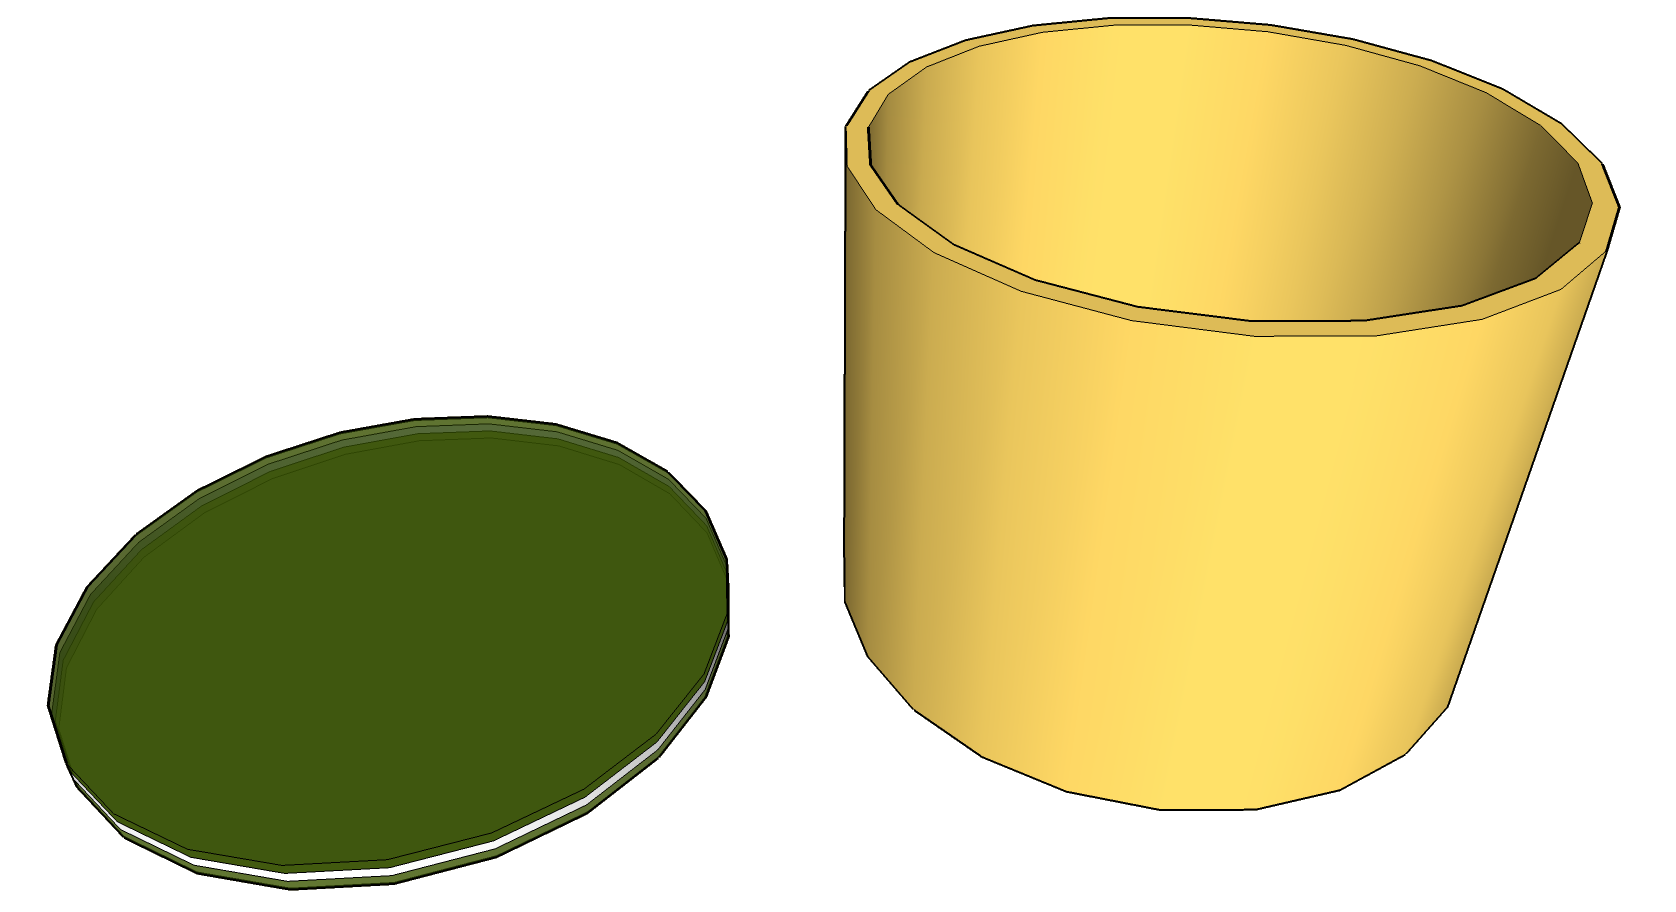
\includegraphics[width=0.838\textwidth,height=0.456\textwidth]{../images/form_factor/anisotropic/localplanar.png}
\end{center}
\caption{for local planar particles the cross section dimension is much smaller then the
radius of curvature of the particle}
\label{fig:localplanar}
\end{figure}

Several cross-section profiles for local planar objects have been implemented,
like a homogeneous cross-section,
cross-section with two infinitely thin plates,
layered centro-symmetric cross-section,
bilayer with a Gaussian scattering length density profile,
layer with Gaussian chains attached to the surface.
These form factors are supposed to be combined with a shape factor for
local planar objects which are implemented as structure  plugins
under "\texttt{[by plugin|anisotropic obj.|P'(Q): local planar
obj.]}".

\clearpage

\subsubsection{Pcs(Q) for a homogeneous cross-section}
\label{plugin:Pcs:homogeneousXS} ~\\

\begin{figure}[htb]
\begin{center}
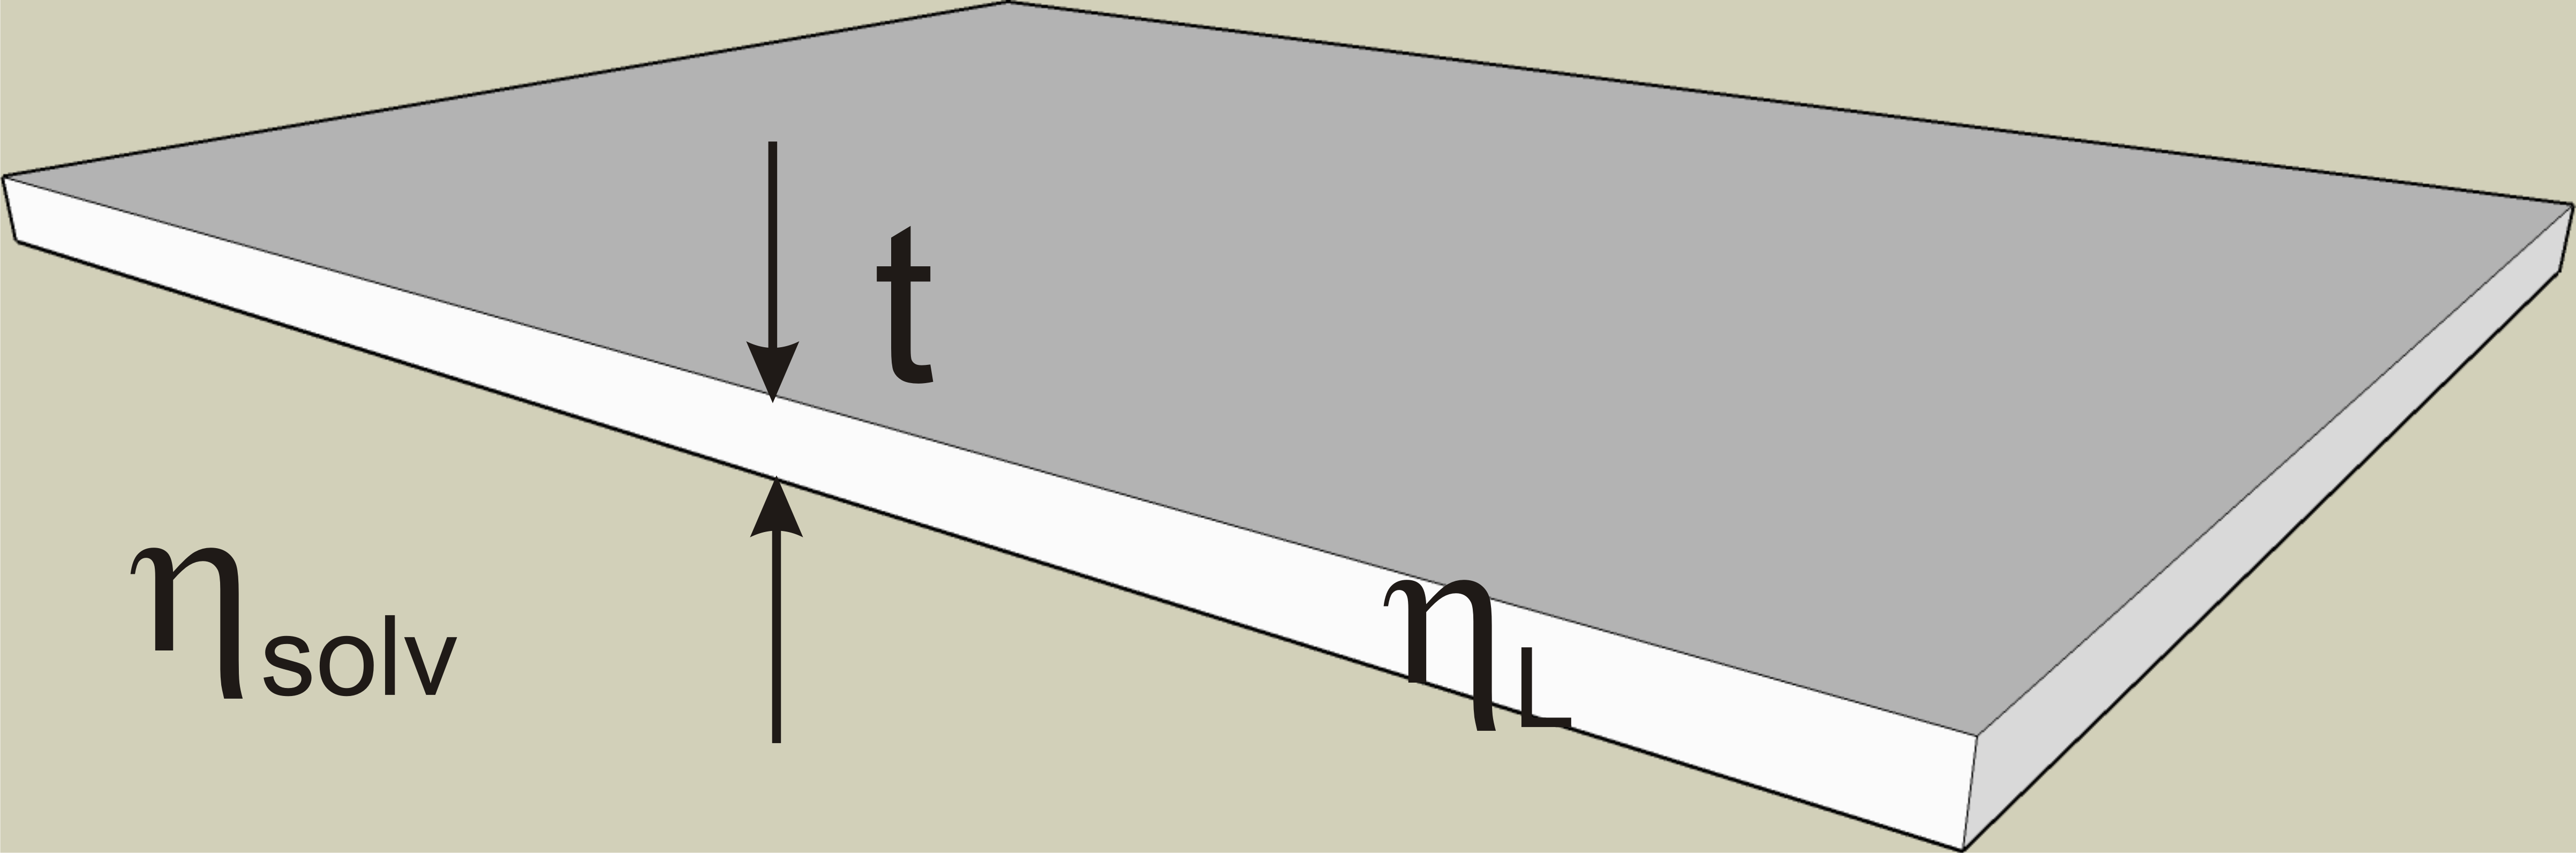
\includegraphics[width=0.802\textwidth,height=0.265\textwidth]{../images/form_factor/anisotropic/Pcs_homogeneousXS_txt.png}
\end{center}
\caption{Plane with a homogeneous cross-section of thickness $t$.}
\label{fig:homogeneousXS}
\end{figure}

This cross-section form factor describes the scattering of a layer with homogeneous
scattering length density $\eta_L$ in a matrix of a scattering length density $\eta_\textrm{solv}$.
The thickness can have a distribution described by a log-normal distribution according to eq.\ \ref{eq:LogNormal}.

\begin{align}
P_\text{cs}(Q,\sigma_{t},t) = \int_0^\infty \textrm{LogNorm}(x,1,\sigma_{t},1,t)
    \left[ \left(\eta_L-\eta_\textrm{solv}\right) x \frac{\sin(Qx/2)}{Qx/2} \right]^2\textrm{d}x
\end{align}

\noindent
\textbf{Input parameters for \texttt{Pcs:homogeneousPlate}:}
\begin{description}
    \item[\texttt{t}] most probable layer thickness $t$
    \item[\texttt{sigm\_t}] width $\sigma_t$ of thickness distribution (LogNorm)
    \item[\texttt{dummy}] unused disabled parameter
    \item[\texttt{dummy}] unused disabled parameter
    \item[\texttt{eta\_l}] scattering length density of layer $\eta_L$
    \item[\texttt{eta\_solv}] scattering length density of solvent $\eta_\textrm{solv}$
\end{description}

\noindent
\textbf{Note}
\begin{itemize}
  \item This form factor is supposed to be combined with a shape factor for
local planar objects which are implemented as structure  plugins
under "\texttt{[by plugin|anisotropic obj.|P'(Q): local planar
obj.]}".
\item As the form factor already have the width distribution included one normally uses in \SASfit as a size distribution
the \texttt{Delta}-distribution.
\end{itemize}

\begin{figure}[htb]
\begin{center}
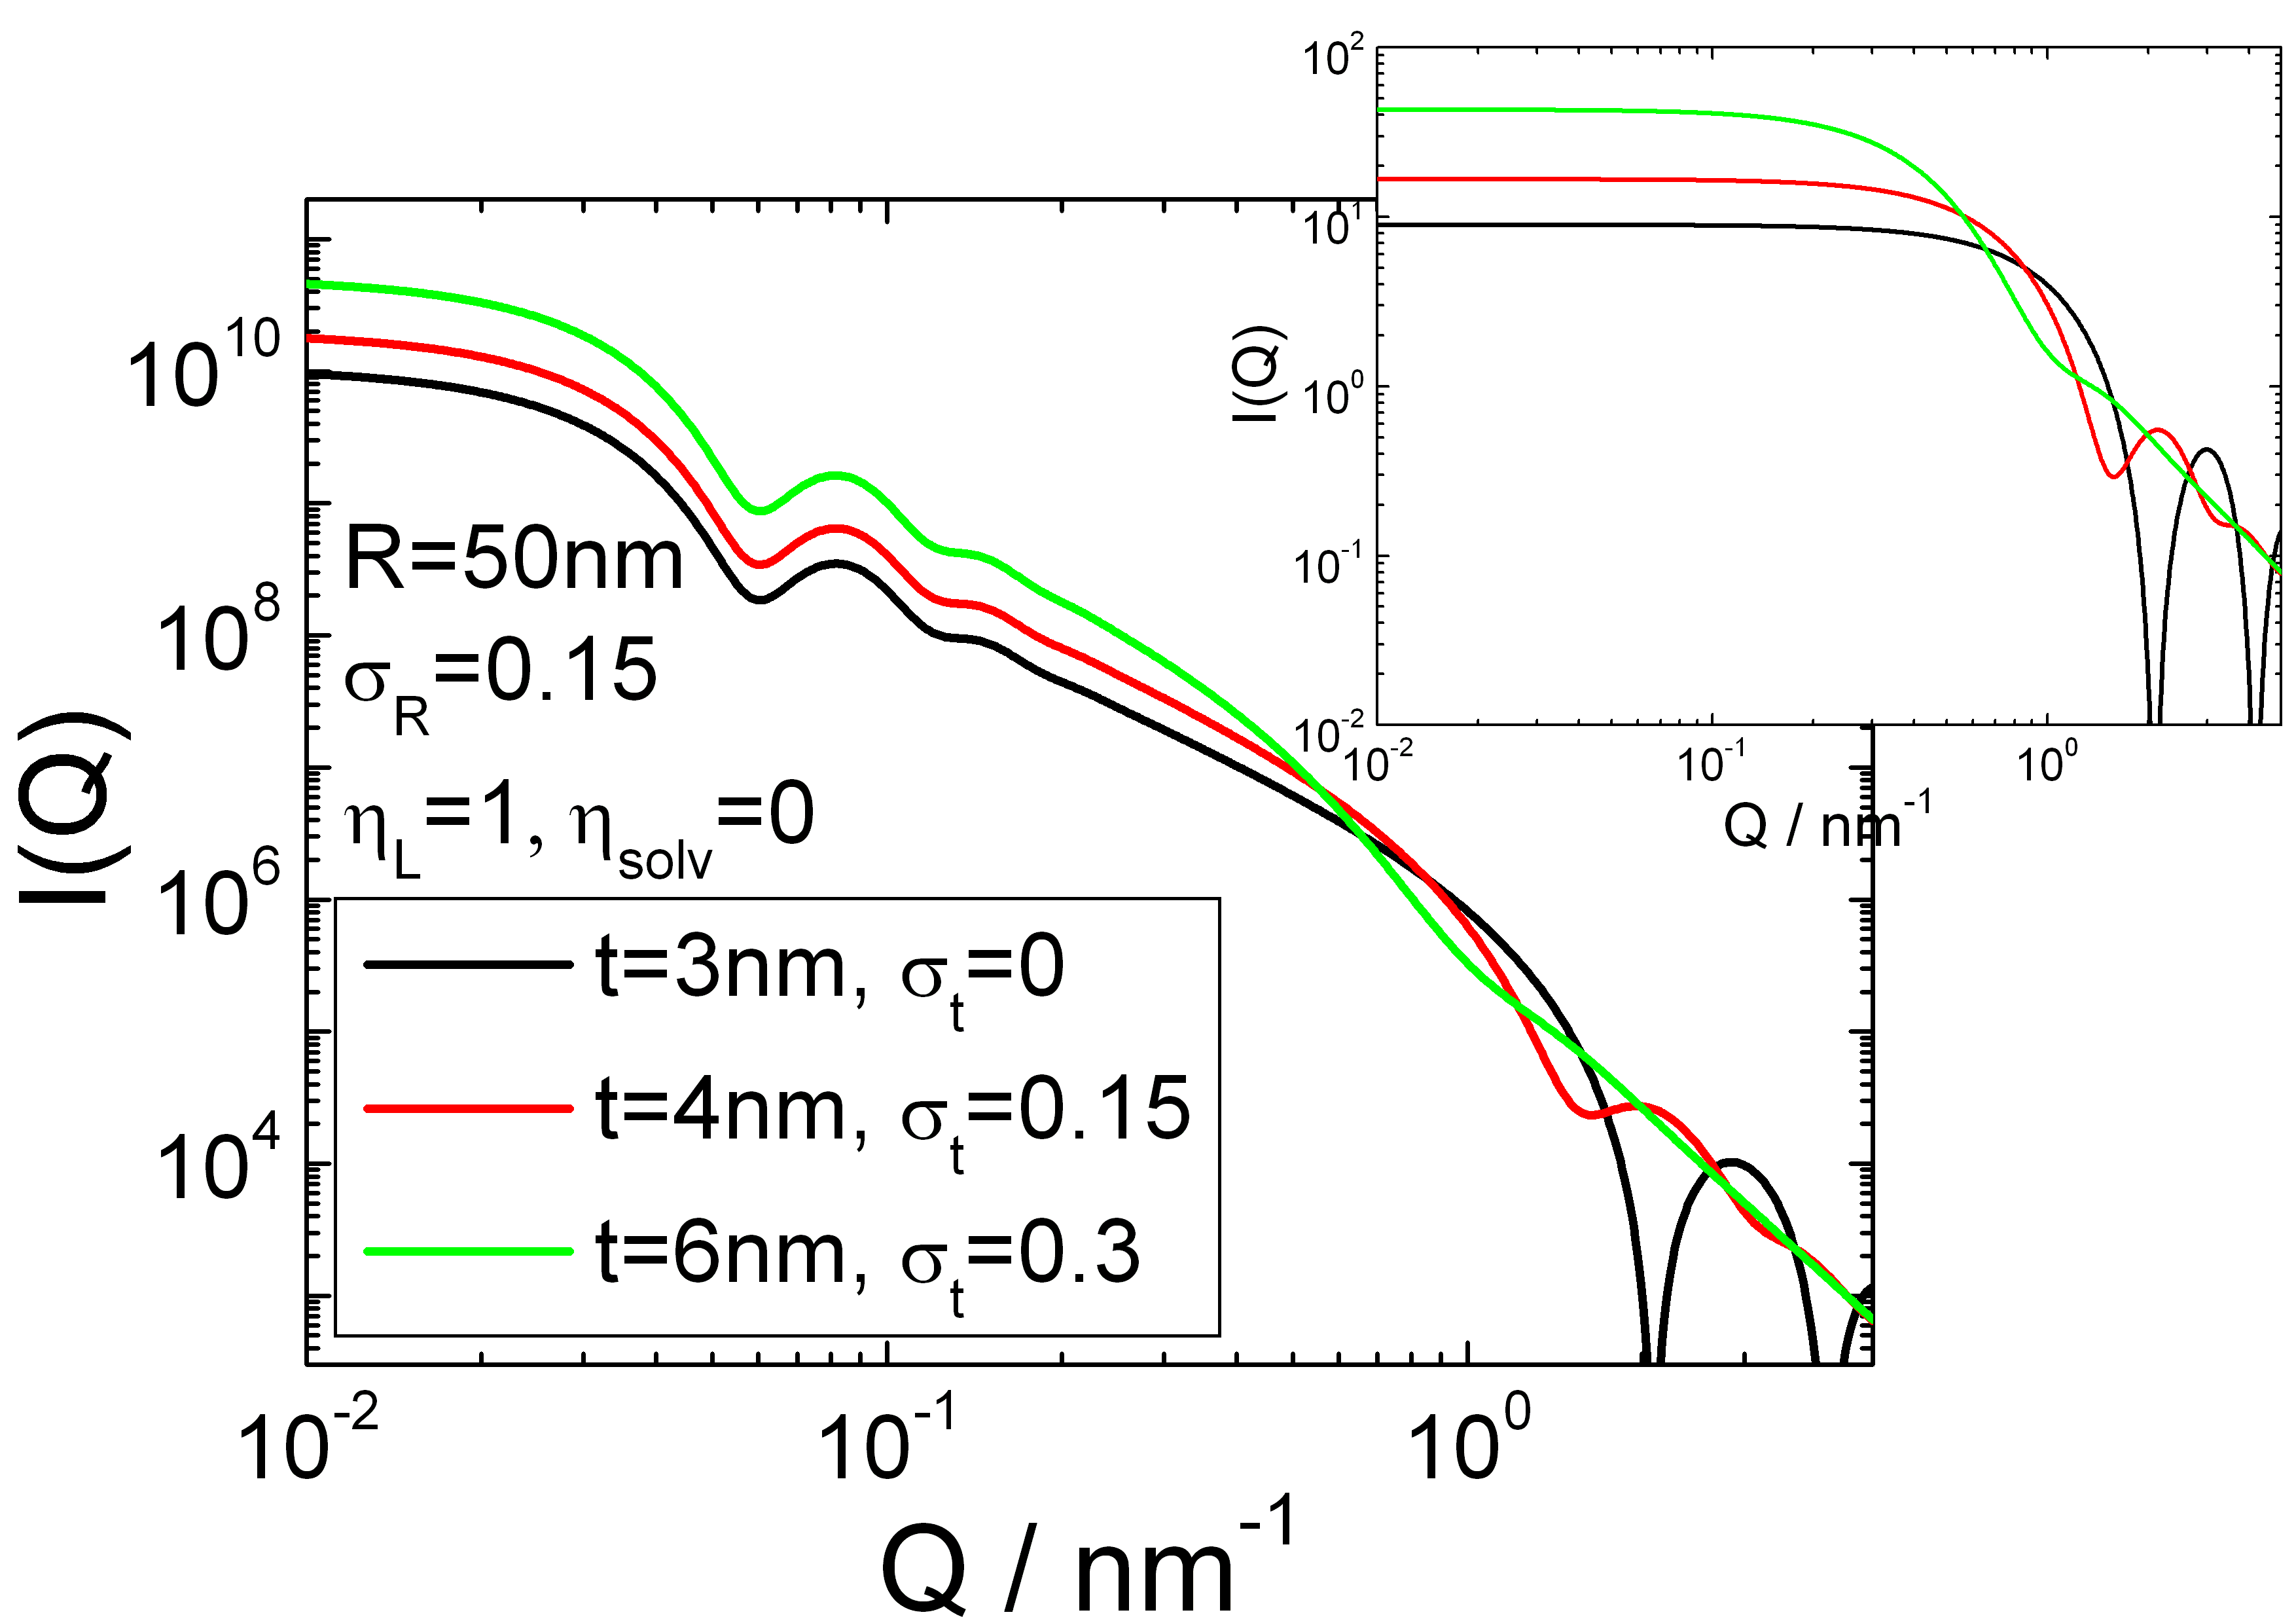
\includegraphics[width=0.8\textwidth,height=0.55\textwidth]{../images/form_factor/anisotropic/localplanarIQ.png}
\end{center}
\caption{Scattering curve for the form factor "\texttt{Pcs:homogeneousPlate}" only (insert) and
in combination with a structure factor "\texttt{P'(Q): Thin Spherical Shell}".}
\label{fig_IQ:homogeneousXS}
\end{figure}

\clearpage
\subsubsection{Pcs(Q) for two infinitely thin parallel layers} ~\\
\label{plugin:Pcs:TwoInfinitelyThinLayers}

\begin{figure}[htb]
\begin{center}
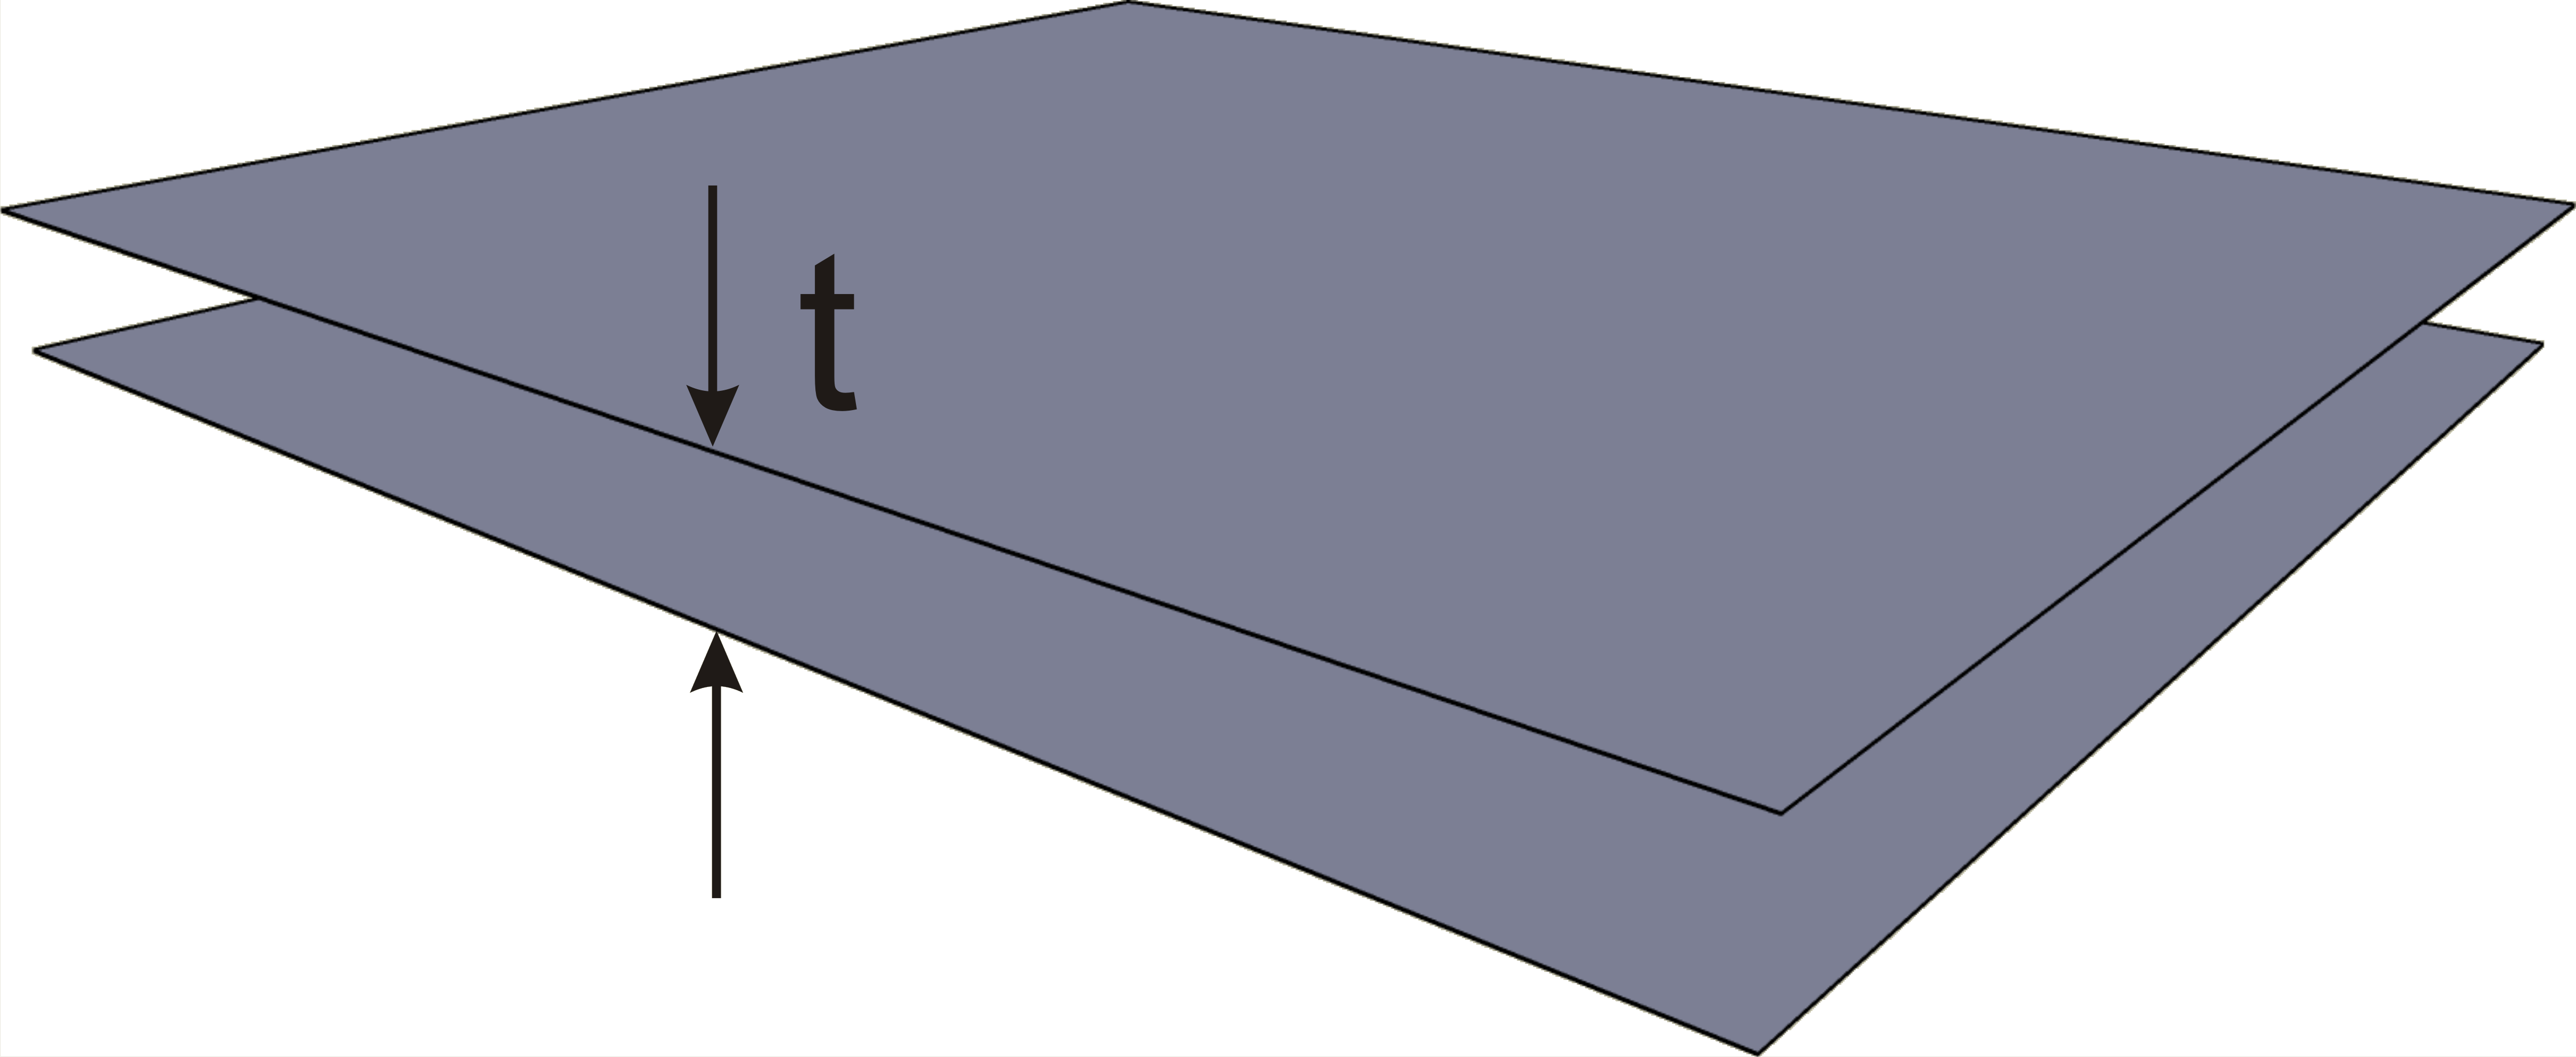
\includegraphics[width=0.8\textwidth,height=0.328\textwidth]{../images/form_factor/anisotropic/planar2thin_txt.png}
\end{center}
\caption{Two infinitely thin parallel layers separated by a distance $t$.}
\label{fig:Pcs:TwoInfinitelyThinLayers}
\end{figure}

This cross-section form factor describes the scattering of two infinitely thin parallel layers.
The separation distance can have a distribution described by a log-normal distribution according
to eq.\ \ref{eq:LogNormal}.

\begin{align}
P_\text{cs}(Q,\sigma_{T},T) = \int_0^\infty \textrm{LogNorm}(x,1,\sigma_{T},1,T) \cos^2(Qx/2) \, \textrm{d}x
\end{align}

\noindent
\textbf{Input parameters for \texttt{Pcs:TwoInfinitelyThinLayers}:}
\begin{description}
    \item[\texttt{t}] most probable layer separation $t$
    \item[\texttt{sigm\_t}] width $\sigma_t$ of separation distribution (LogNorm)
\end{description}

\noindent
\textbf{Note}
\begin{itemize}
  \item This form factor is supposed to be combined with a shape factor for
local planar objects which are implemented as structure  plugins
under "\texttt[{by plugin|anisotropic obj.|P'(Q): local planar
obj.]}".
\item As the form factor already have the width distribution included one normally uses in \SASfit as a size distribution
the \texttt{Delta}-distribution.
\end{itemize}

\begin{figure}[htb]
\begin{center}
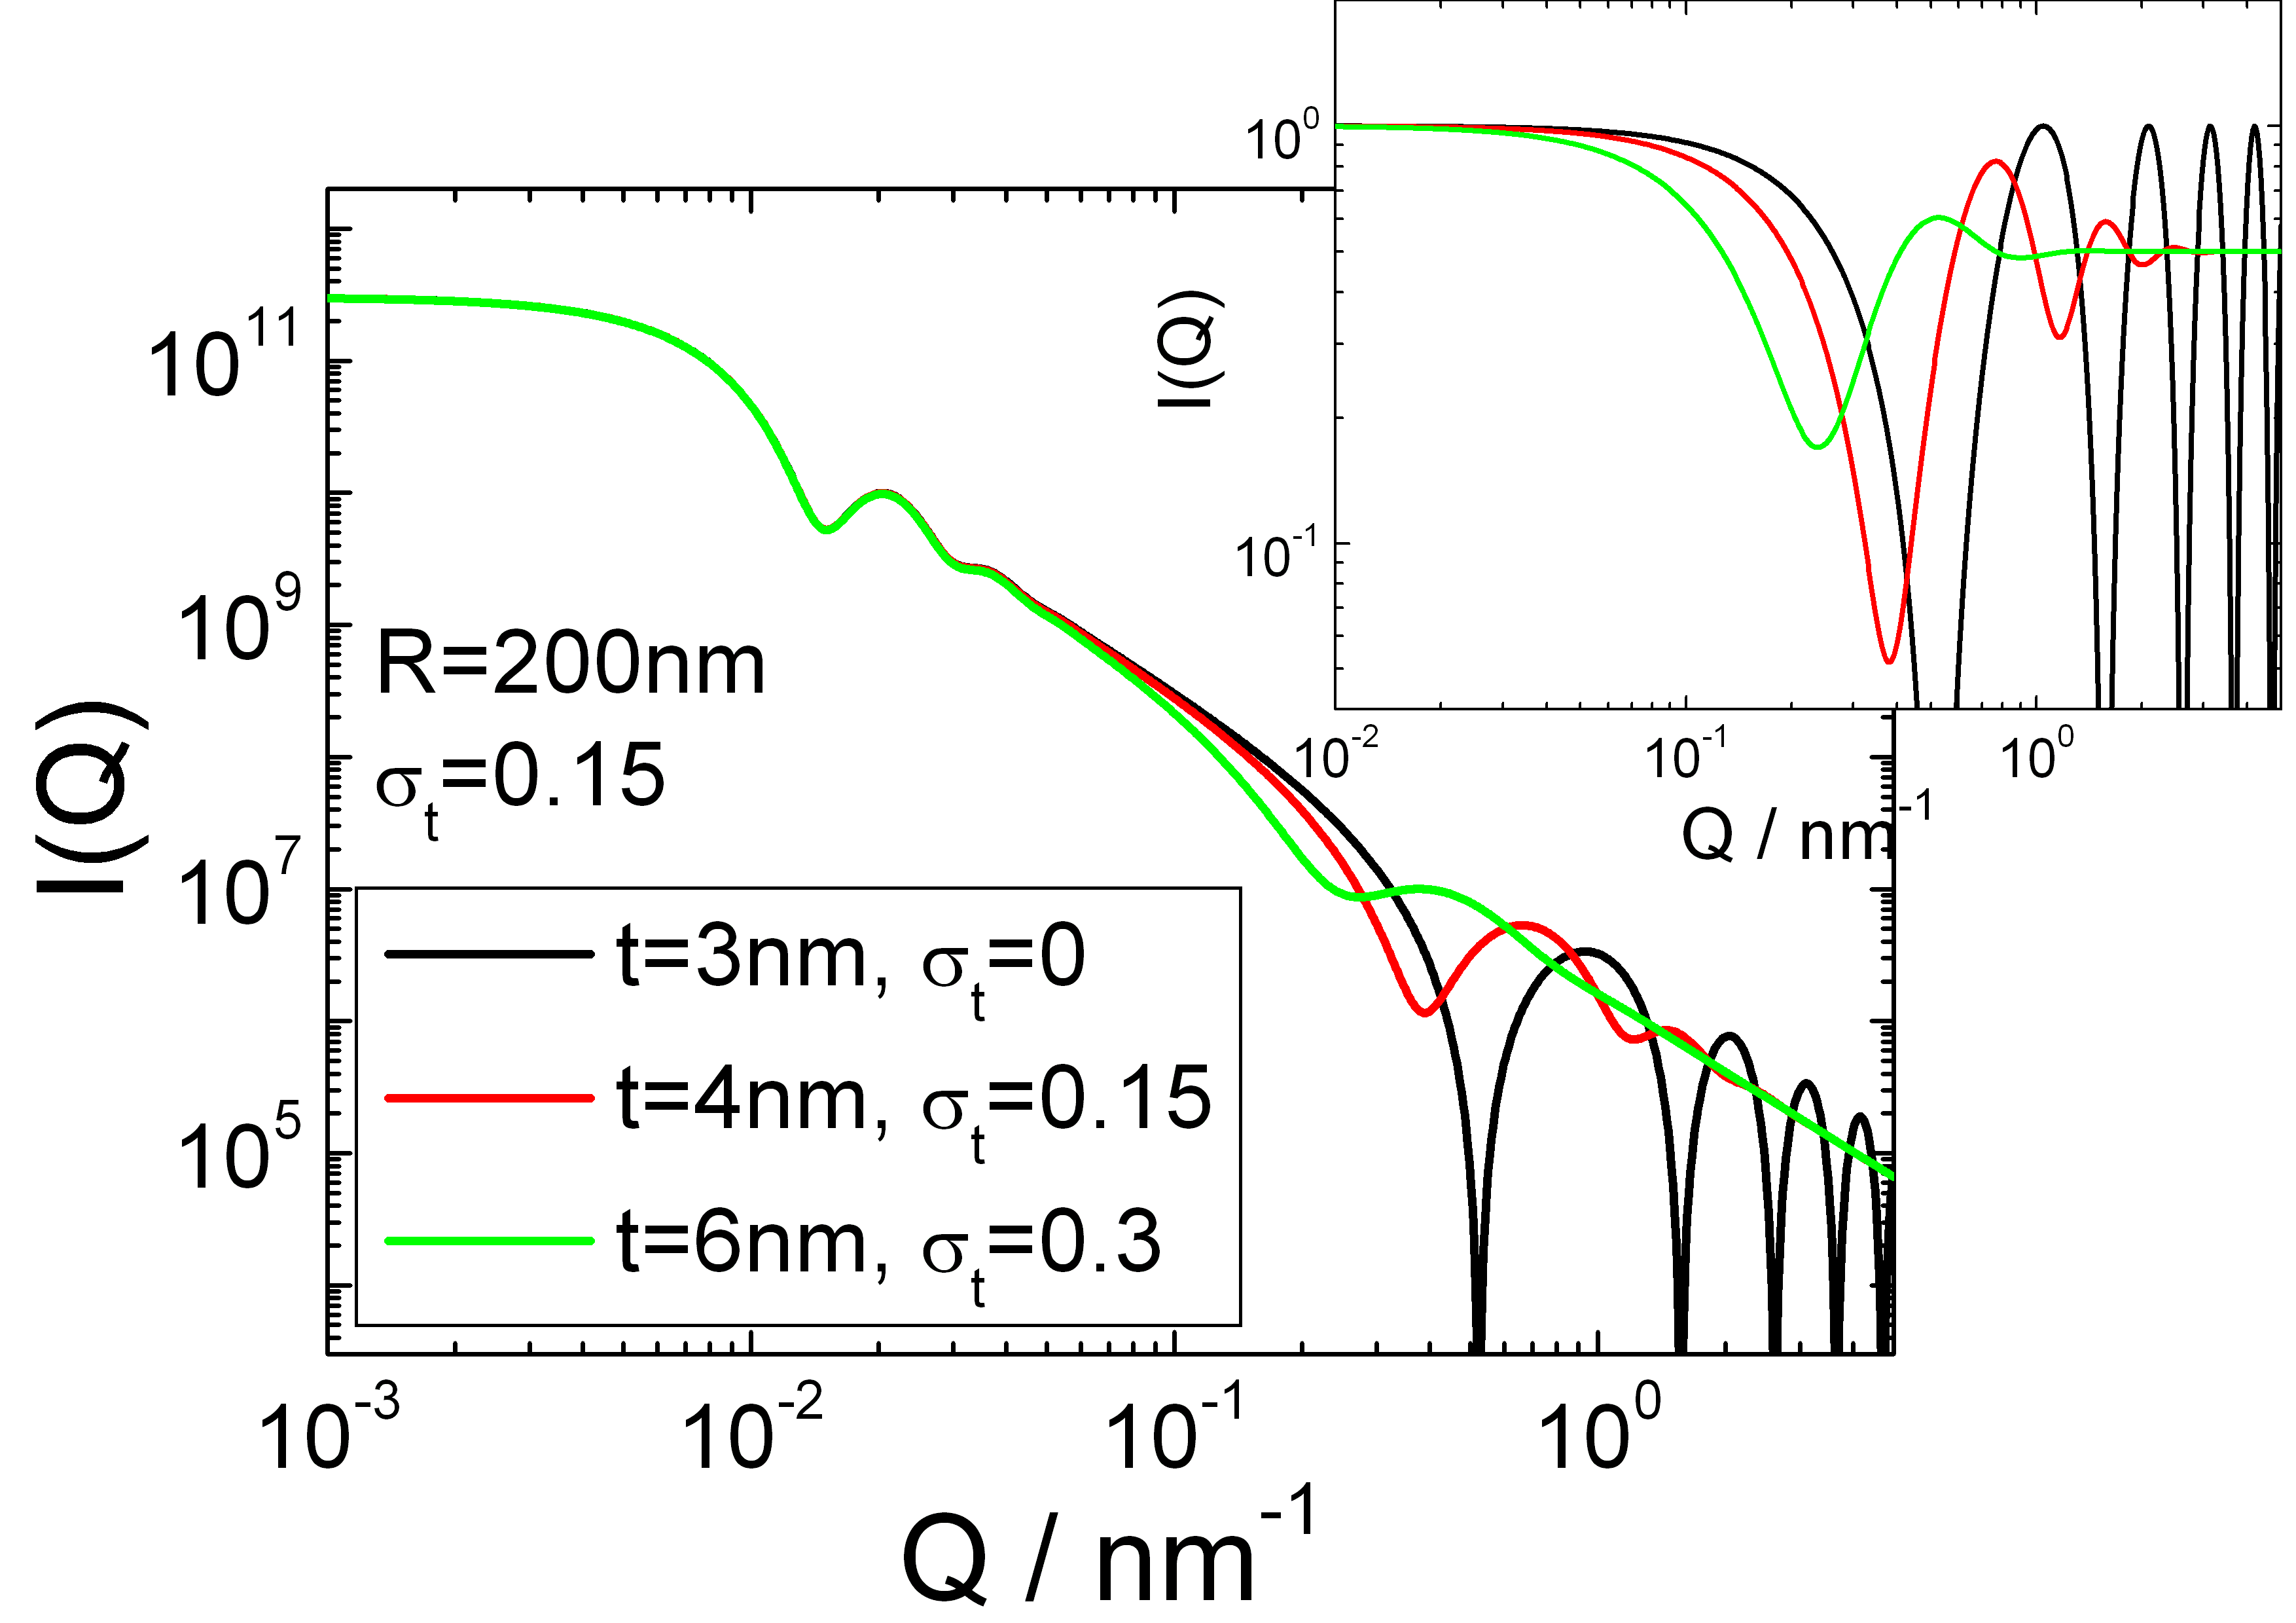
\includegraphics[width=0.8\textwidth,height=0.55\textwidth]{../images/form_factor/anisotropic/planar2thinIQ.png}
\end{center}
\caption{Scattering curve for the form factor "\texttt{Pcs:TwoInfinitelyThinLayers}" only (insert) and
in combination with a structure factor "\texttt{P'(Q): Thin Spherical Shell}".}
\label{fig_IQ:Pcs:TwoInfinitelyThinLayers}
\end{figure}


\clearpage
\subsubsection{Pcs(Q) for a layered centro symmetric cross-section structure} ~\\
\label{plugin:Pcs:LayeredCentroSymmetricCrossSectionStructure}

\begin{figure}[htb]
\begin{center}
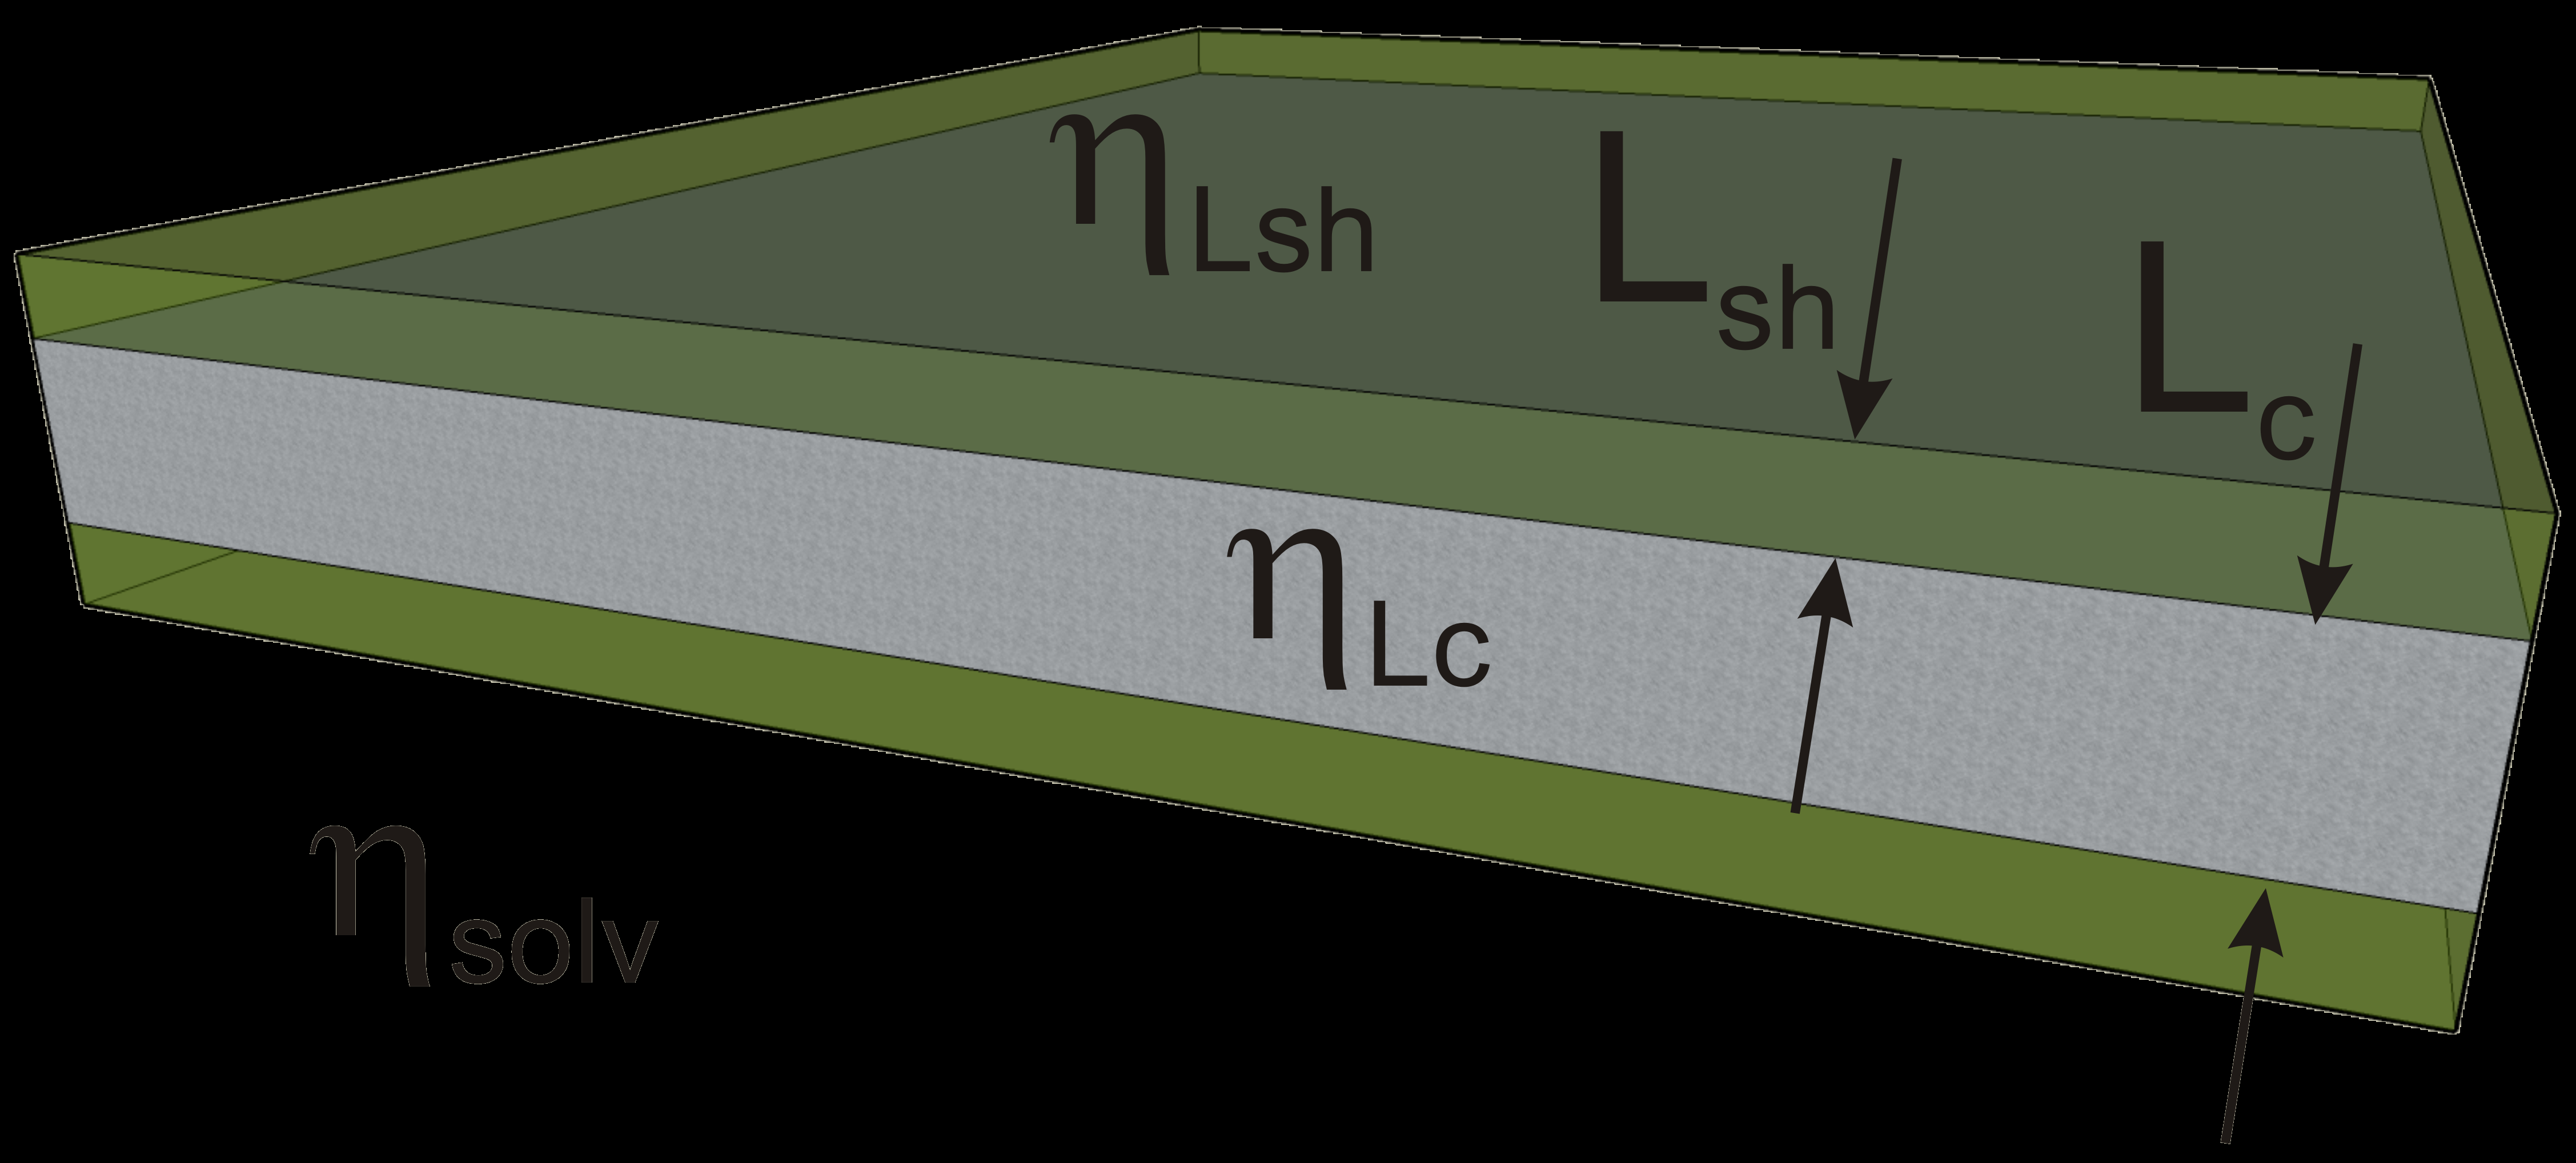
\includegraphics[width=0.8\textwidth,height=0.361\textwidth]{../images/form_factor/anisotropic/planar2centrosymm_txt.png}
\end{center}
\caption{Two layered centro symmetric structure with a core thickness of $L_\textrm{c}$ and an outer layer thickness
$L_{L_\textrm{sh}}$. The corresponding scattering length densities of the core, the shell layer and the solvent are
$L_{L_\textrm{c}}$, $L_{L_\textrm{sh}}$, and $L_{L_\textrm{solv}}$.}
\label{fig:Pcs:TwoInfinitelyThinLayers}
\end{figure}

This cross-section form factor describes the scattering of a layered centro symmetric cross-section structure.
Both the core thickness as well as the shell thickness can have a distribution described by a log-normal distribution as defined in eq.\ \ref{eq:LogNormal}.

\begin{multline}
P_\text{cs}(Q,\sigma_{L_\textrm{c}},L_\textrm{c},\sigma_{L_\textrm{sh}},L_\textrm{sh},\eta_{L_\textrm{c}},\eta_{L_\textrm{sh}},\eta_\textrm{sol}) = \\
\int_0^\infty \textrm{LogNorm}(v,1,\sigma_{L_\textrm{c}},1,L_\textrm{c})
\int_0^\infty \textrm{LogNorm}(u,1,\sigma_{L_\textrm{sh}},1,L_\textrm{sh}) \\
     \Bigg[ \frac{(\eta_{L_\textrm{sh}}-\eta_\textrm{solv})(v+2u) \sin\left(Q\frac{v+2u}{2}\right)}{Q\frac{v+2u}{2}}
          -\frac{(\eta_{L_\textrm{sh}}-\eta_{L_\textrm{c}})  v   \sin\left(Q \frac{v}{2}\right)}{Q \frac{v}{2}}
    \Bigg]^2 \,
\textrm{d}u \, \textrm{d}v
\end{multline}

\noindent
\textbf{Input parameters for \texttt{Pcs:LayeredCentroSymmetricXS}:}
\begin{description}
    \item[\texttt{L\_c}] most probable layer separation $L_\textrm{c}$
    \item[\texttt{sigm\_Lc}] width $\sigma_{L_\textrm{c}}$ of core thickness distribution (LogNorm)
    \item[\texttt{L\_sh}] most probable shell thickness $L_\textrm{sh}$
    \item[\texttt{sigm\_Lsh}] width $\sigma_{L_\textrm{c}}$ of shell thickness distribution (LogNorm)
    \item[\texttt{eta\_Lc}] scattering length density of core layer $\eta_{L_\textrm{c}}$
    \item[\texttt{eta\_Lsh}] scattering length density of shell layer $\eta_{L_\textrm{sh}}$
    \item[\texttt{eta\_solv}] scattering length density of solvent $\eta_{solv}$
\end{description}

\noindent
\textbf{Note}
\begin{itemize}
  \item This form factor is supposed to be combined with a shape factor for
local planar objects which are implemented as structure  plugins
under "\texttt{[by plugin|anisotropic obj.|P'(Q): local planar
obj.]}".
\item As the form factor already have the width distribution included one normally uses in \SASfit as a size distribution
the \texttt{Delta}-distribution.
\end{itemize}

\begin{figure}[htb]
\begin{center}
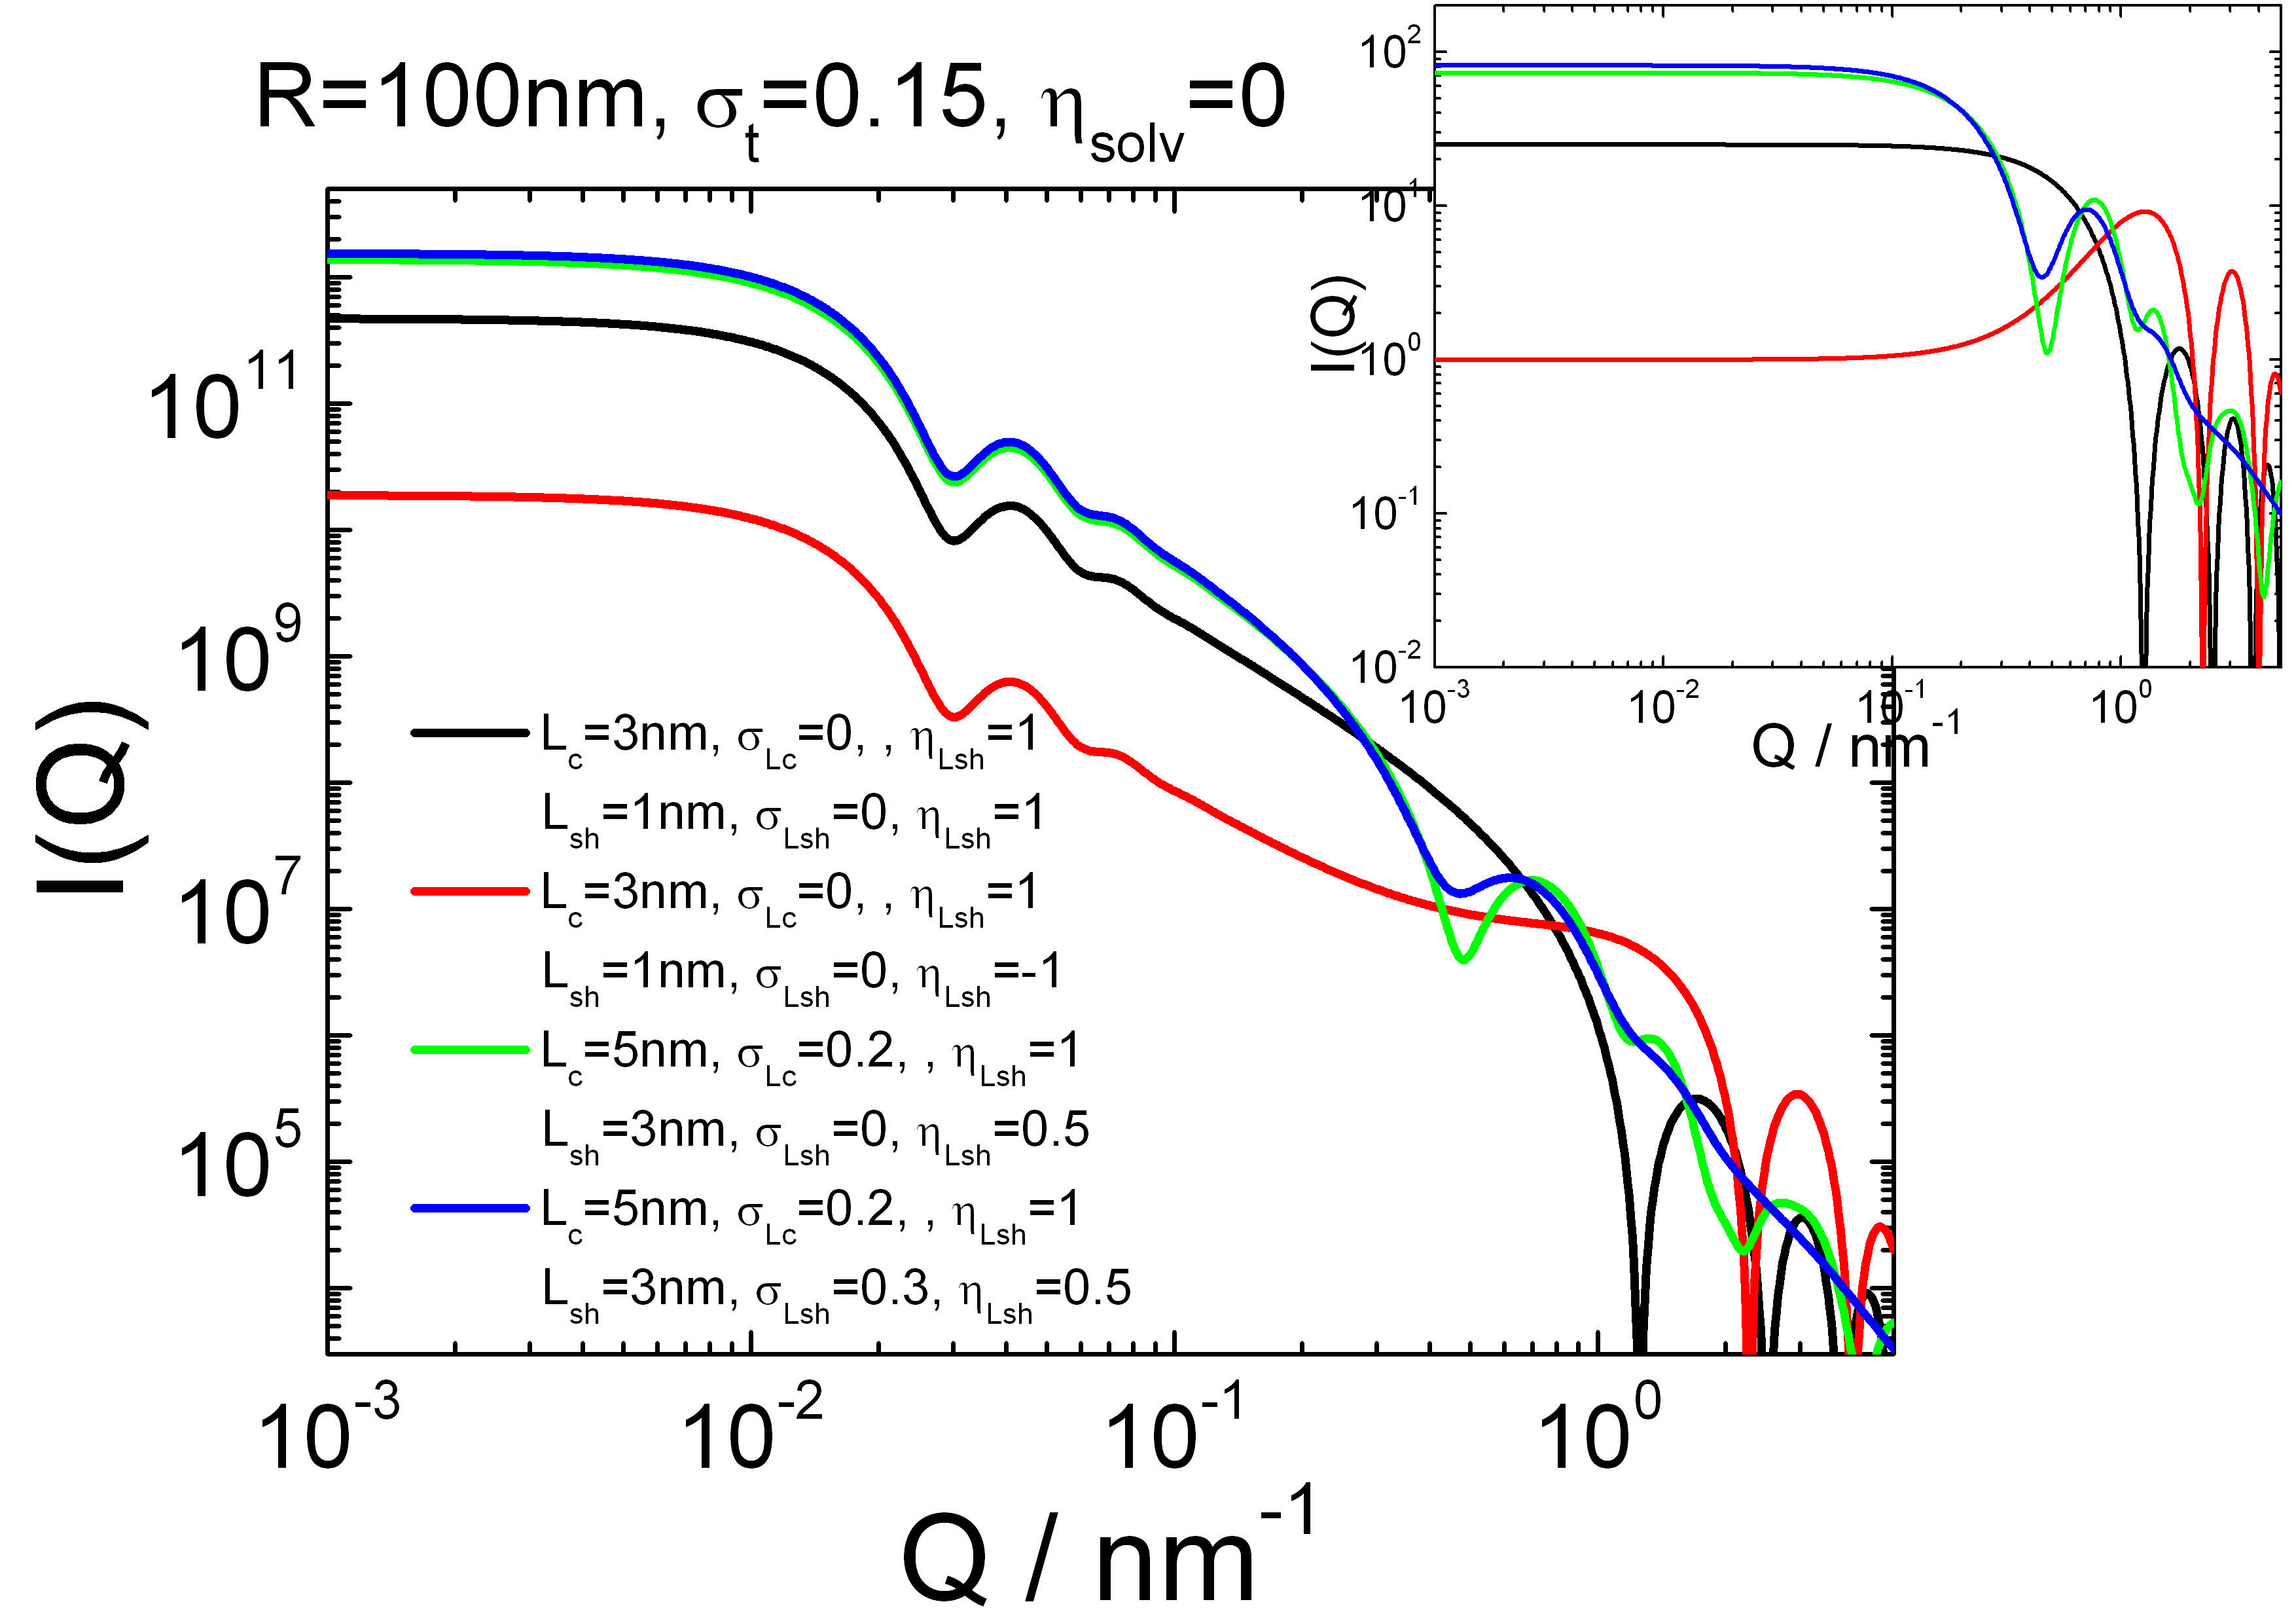
\includegraphics[width=0.8\textwidth,height=0.55\textwidth]{../images/form_factor/anisotropic/Pcs_planar2centrosymmIQ.png}
\end{center}
\caption{Scattering curve for the form factor "\texttt{Pcs:LayeredCentroSymmetricXS}" only (insert) and
in combination with a structure factor "\texttt{P'(Q): Thin Spherical Shell}".}
\label{fig:Pcs_planar2centrosymmIQ}
\end{figure}

\clearpage

\subsubsection{Pcs(Q) for a bilayer with a Gaussian electron density profile \cite{Pabst2000,Pabst2003}} ~\\
\label{plugin:Pcs:GaussianProfile}

\begin{figure}[htb]
\begin{center}
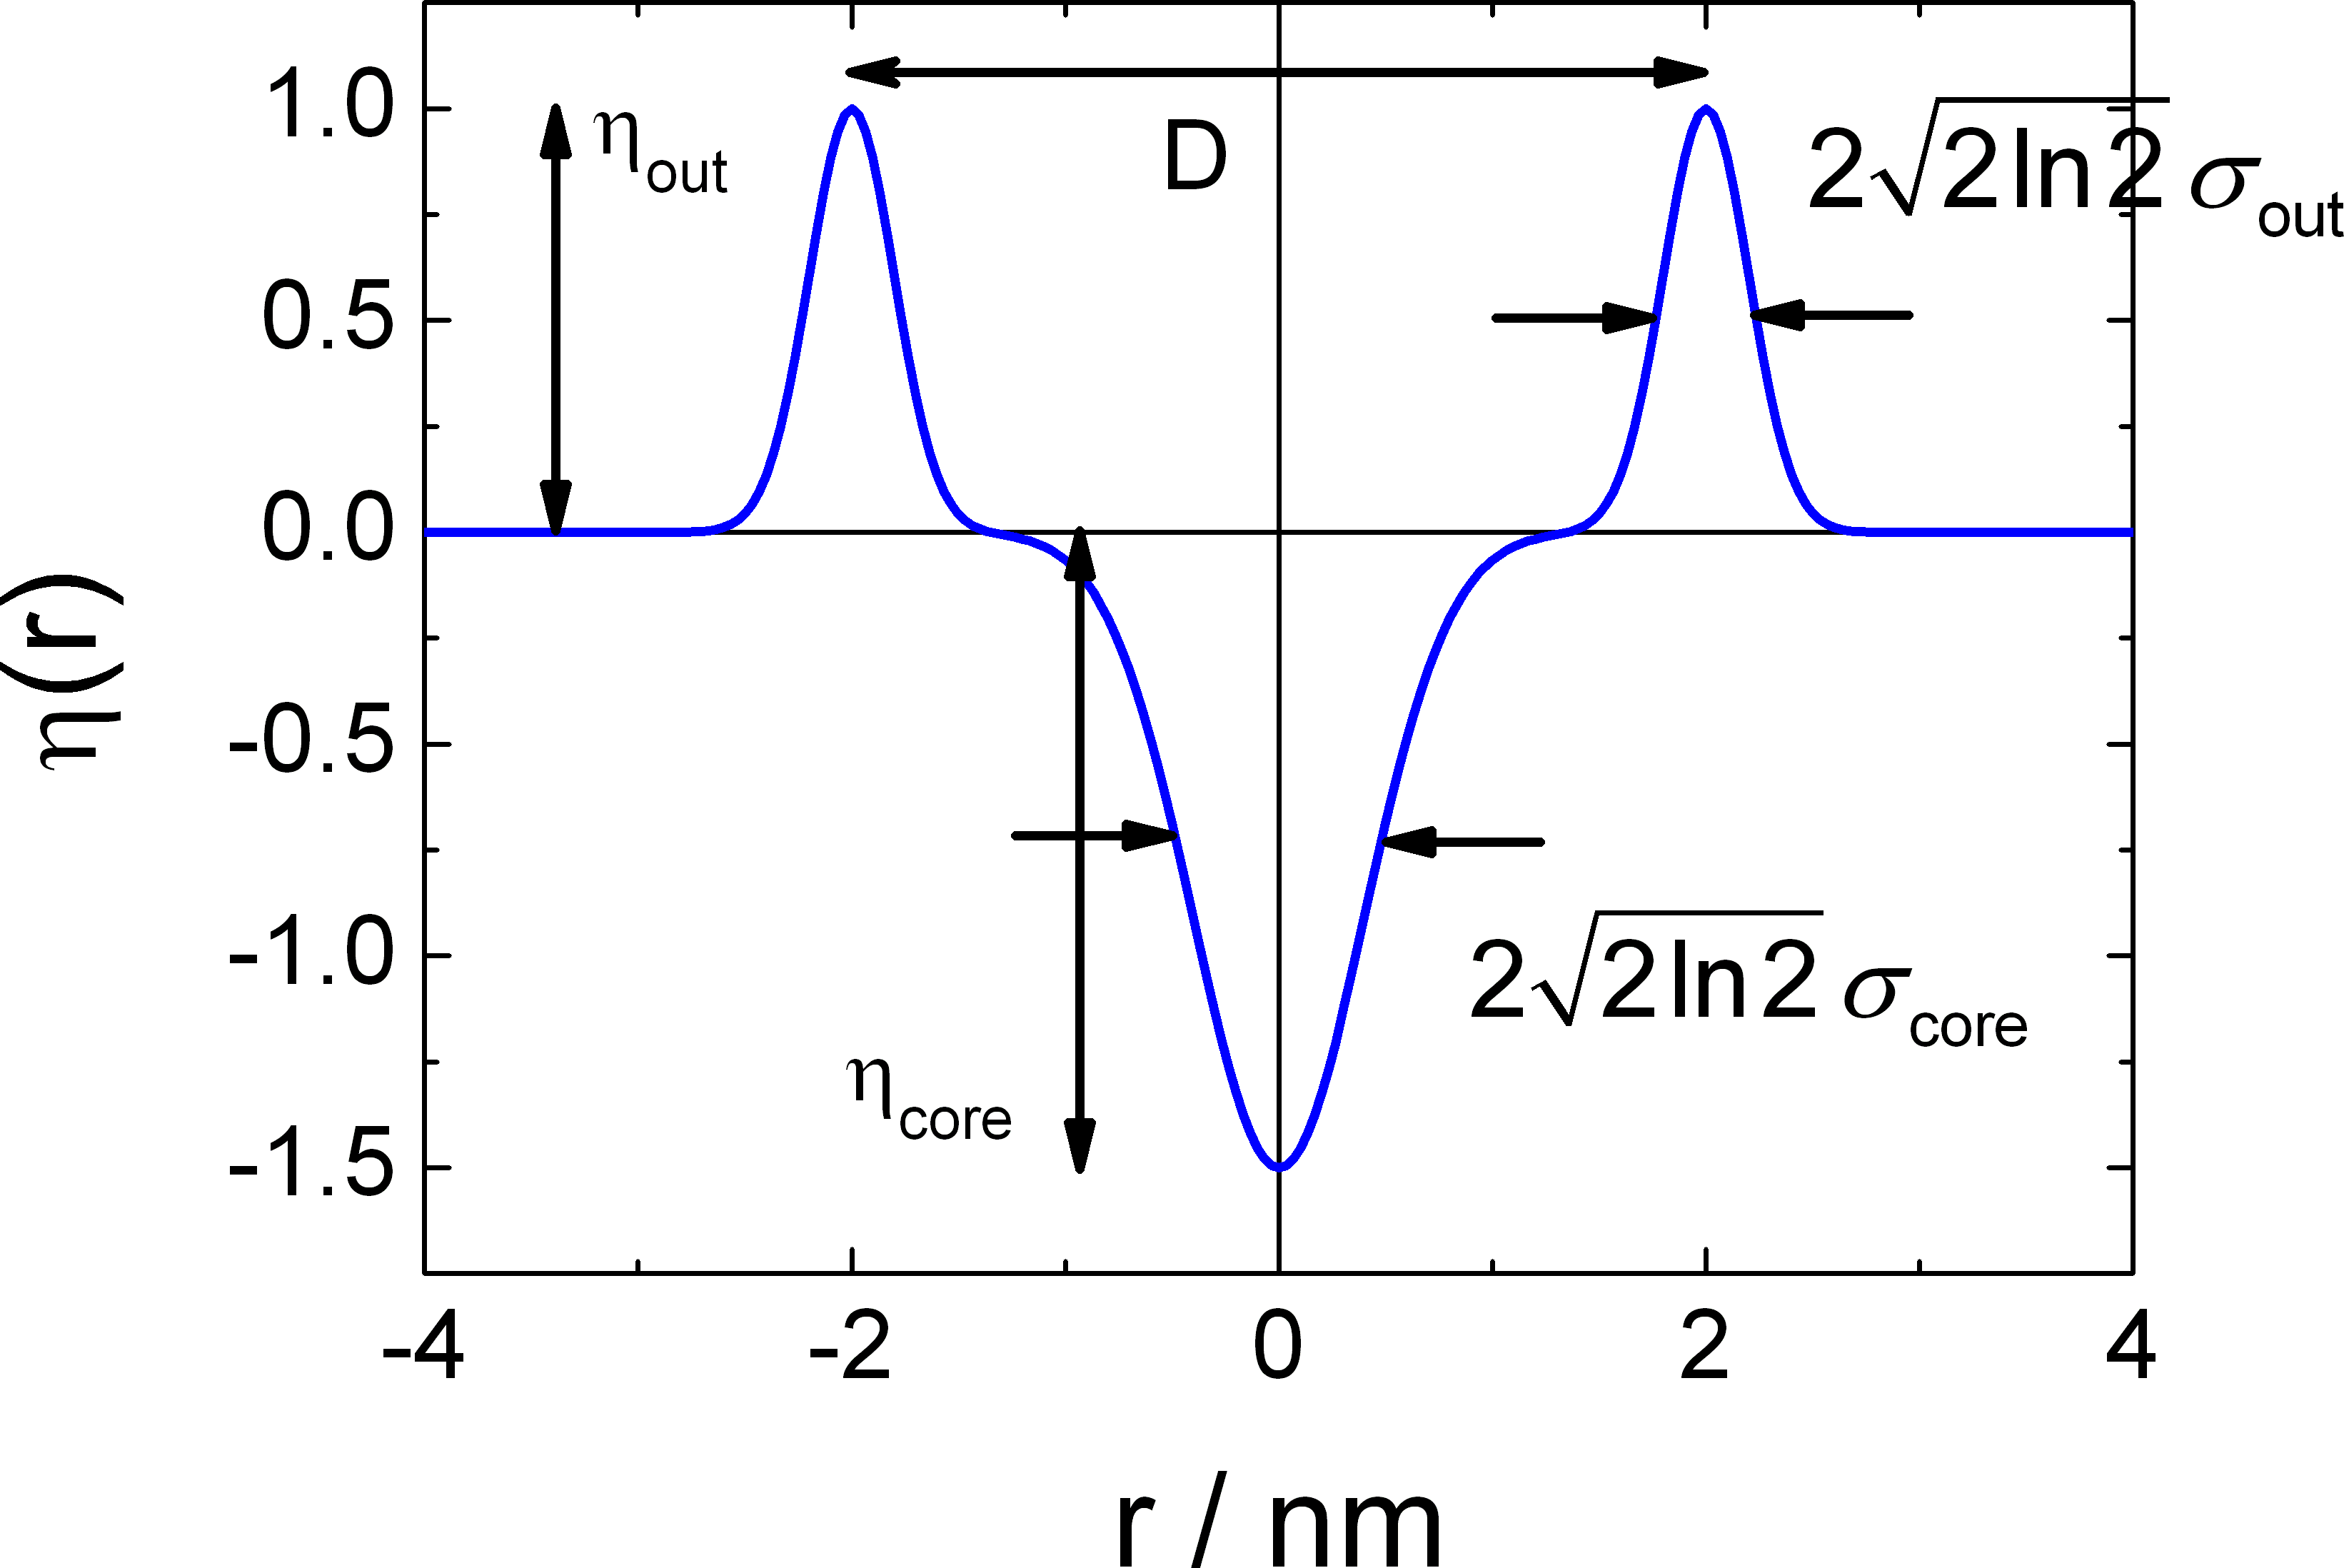
\includegraphics[width=0.8\textwidth,height=0.55\textwidth]{../images/form_factor/anisotropic/BiLayerGauss_Profile.png}
\end{center}
\caption{
The plot shows a model for the Gaussian description of the bilayer electron density profile according to
eq.\ \ref{eq:BiLayerGaussianProfile}.
The origin of the profile is set to the bilayer centre. The model encountering a single Gaussian for the head
group at $\pm t/2$. $\eta_\textrm{out}$ is the amplitude of the headgroup Gaussian and $\eta_\textrm{core}$ that of
the hydrocarbon chains with respect to the average electron density of water. The FWHM of the Gaussian profiles are
$2\sqrt{2\ln 2}\sigma_\textrm{out}$ and $2\sqrt{2\ln 2}\sigma_\textrm{core}$.}
\label{fig:bilayerprofile}
\end{figure}

This model for a bilayer is using a real-space representation of the electron density profile
using a Gaussian description \cite{Pabst2000,Pabst2003}. In comparison to other models it
is simpler and requiring the adjustment of only four parameters. The electron density profile
(Fig.\ \ref{fig:bilayerprofile}) is described by
\begin{align}
\begin{split}
\eta(r) &=  \eta_\textrm{out} \left[ \exp\left(-\frac{\left(r-\frac{t}{2}\right)^2}{2\sigma_\textrm{out}^2}\right) +
   \exp\left(-\frac{\left(r+\frac{t}{2}\right)^2}{2\sigma_\textrm{out}^2}\right) \right] \\
          &+ \eta_\textrm{core} \exp\left(-\frac{r^2}{2\sigma_\textrm{core}^2}\right)
          \label{eq:BiLayerGaussianProfile}
\end{split}
\end{align}
The scattering intensity of this cross section profile of a planar object can be calculated by eq.\ \ref{Pcs:planar}
and computes as
\begin{align}
   F_\text{out}\left(Q,D,\sigma_\textrm{out},\eta_\textrm{out}\right)  &= \sqrt{2\pi}\sigma_\textrm{out}  \eta_\textrm{out}  \exp\left(-\frac{1}{2}\left(Q\sigma_\textrm{out} \right)^2\right) \cos\left(Q\frac{t}{2}\right) \\
   F_\text{core}\left(Q,\sigma_\textrm{core},\eta_\textrm{core}\right) &= \sqrt{2\pi}\sigma_\textrm{core} \eta_\textrm{core} \exp\left(-\frac{1}{2}\left(Q\sigma_\textrm{core}\right)^2\right)
\end{align}
so that
\begin{align}
  P_\text{cs}\left(Q\right)   &=\left[F_\text{core}\left(Q,\sigma_\textrm{core}, \eta_\textrm{core}\right)
                                   +2 F_\text{out} \left(Q,D,\sigma_\textrm{out},\eta_\textrm{out} \right)\right]^2
  \label{eq:PcsBilayer}
\end{align}

\noindent
\textbf{Input parameters for \texttt{Pcs:BilayerGauss}:}
\begin{description}
    \item[\texttt{sigma\_core}] width $\sigma_\mathrm{out}$ of the central Gaussian profile
    \item[\texttt{eta\_core}] scattering length density contrast of the central Gaussian profile
    \item[\texttt{sigma\_out}] width $\sigma_\mathrm{out}$ of the two outer Gaussian profiles
    \item[\texttt{eta\_out}] scattering length density contrast of the two outer Gaussian profiles
    \item[\texttt{t}] distance between the centers of the outer Gaussian profiles
\end{description}

\noindent
\textbf{Note}
\begin{itemize}
  \item This form factor is supposed to be combined with a shape factor for
local planar objects which are implemented as structure  plugins
under "\texttt{[by plugin|anisotropic obj.|P'(Q): local planar
obj.]}".
\end{itemize}

\begin{figure}[htb]
\begin{center}
\subfigure[Plot of the cross section form factor $P_\text{cs}$ in combination with a structure factor "\texttt{P'(Q): Thin Disc}"
as the shape factor $P'(Q)$.]{
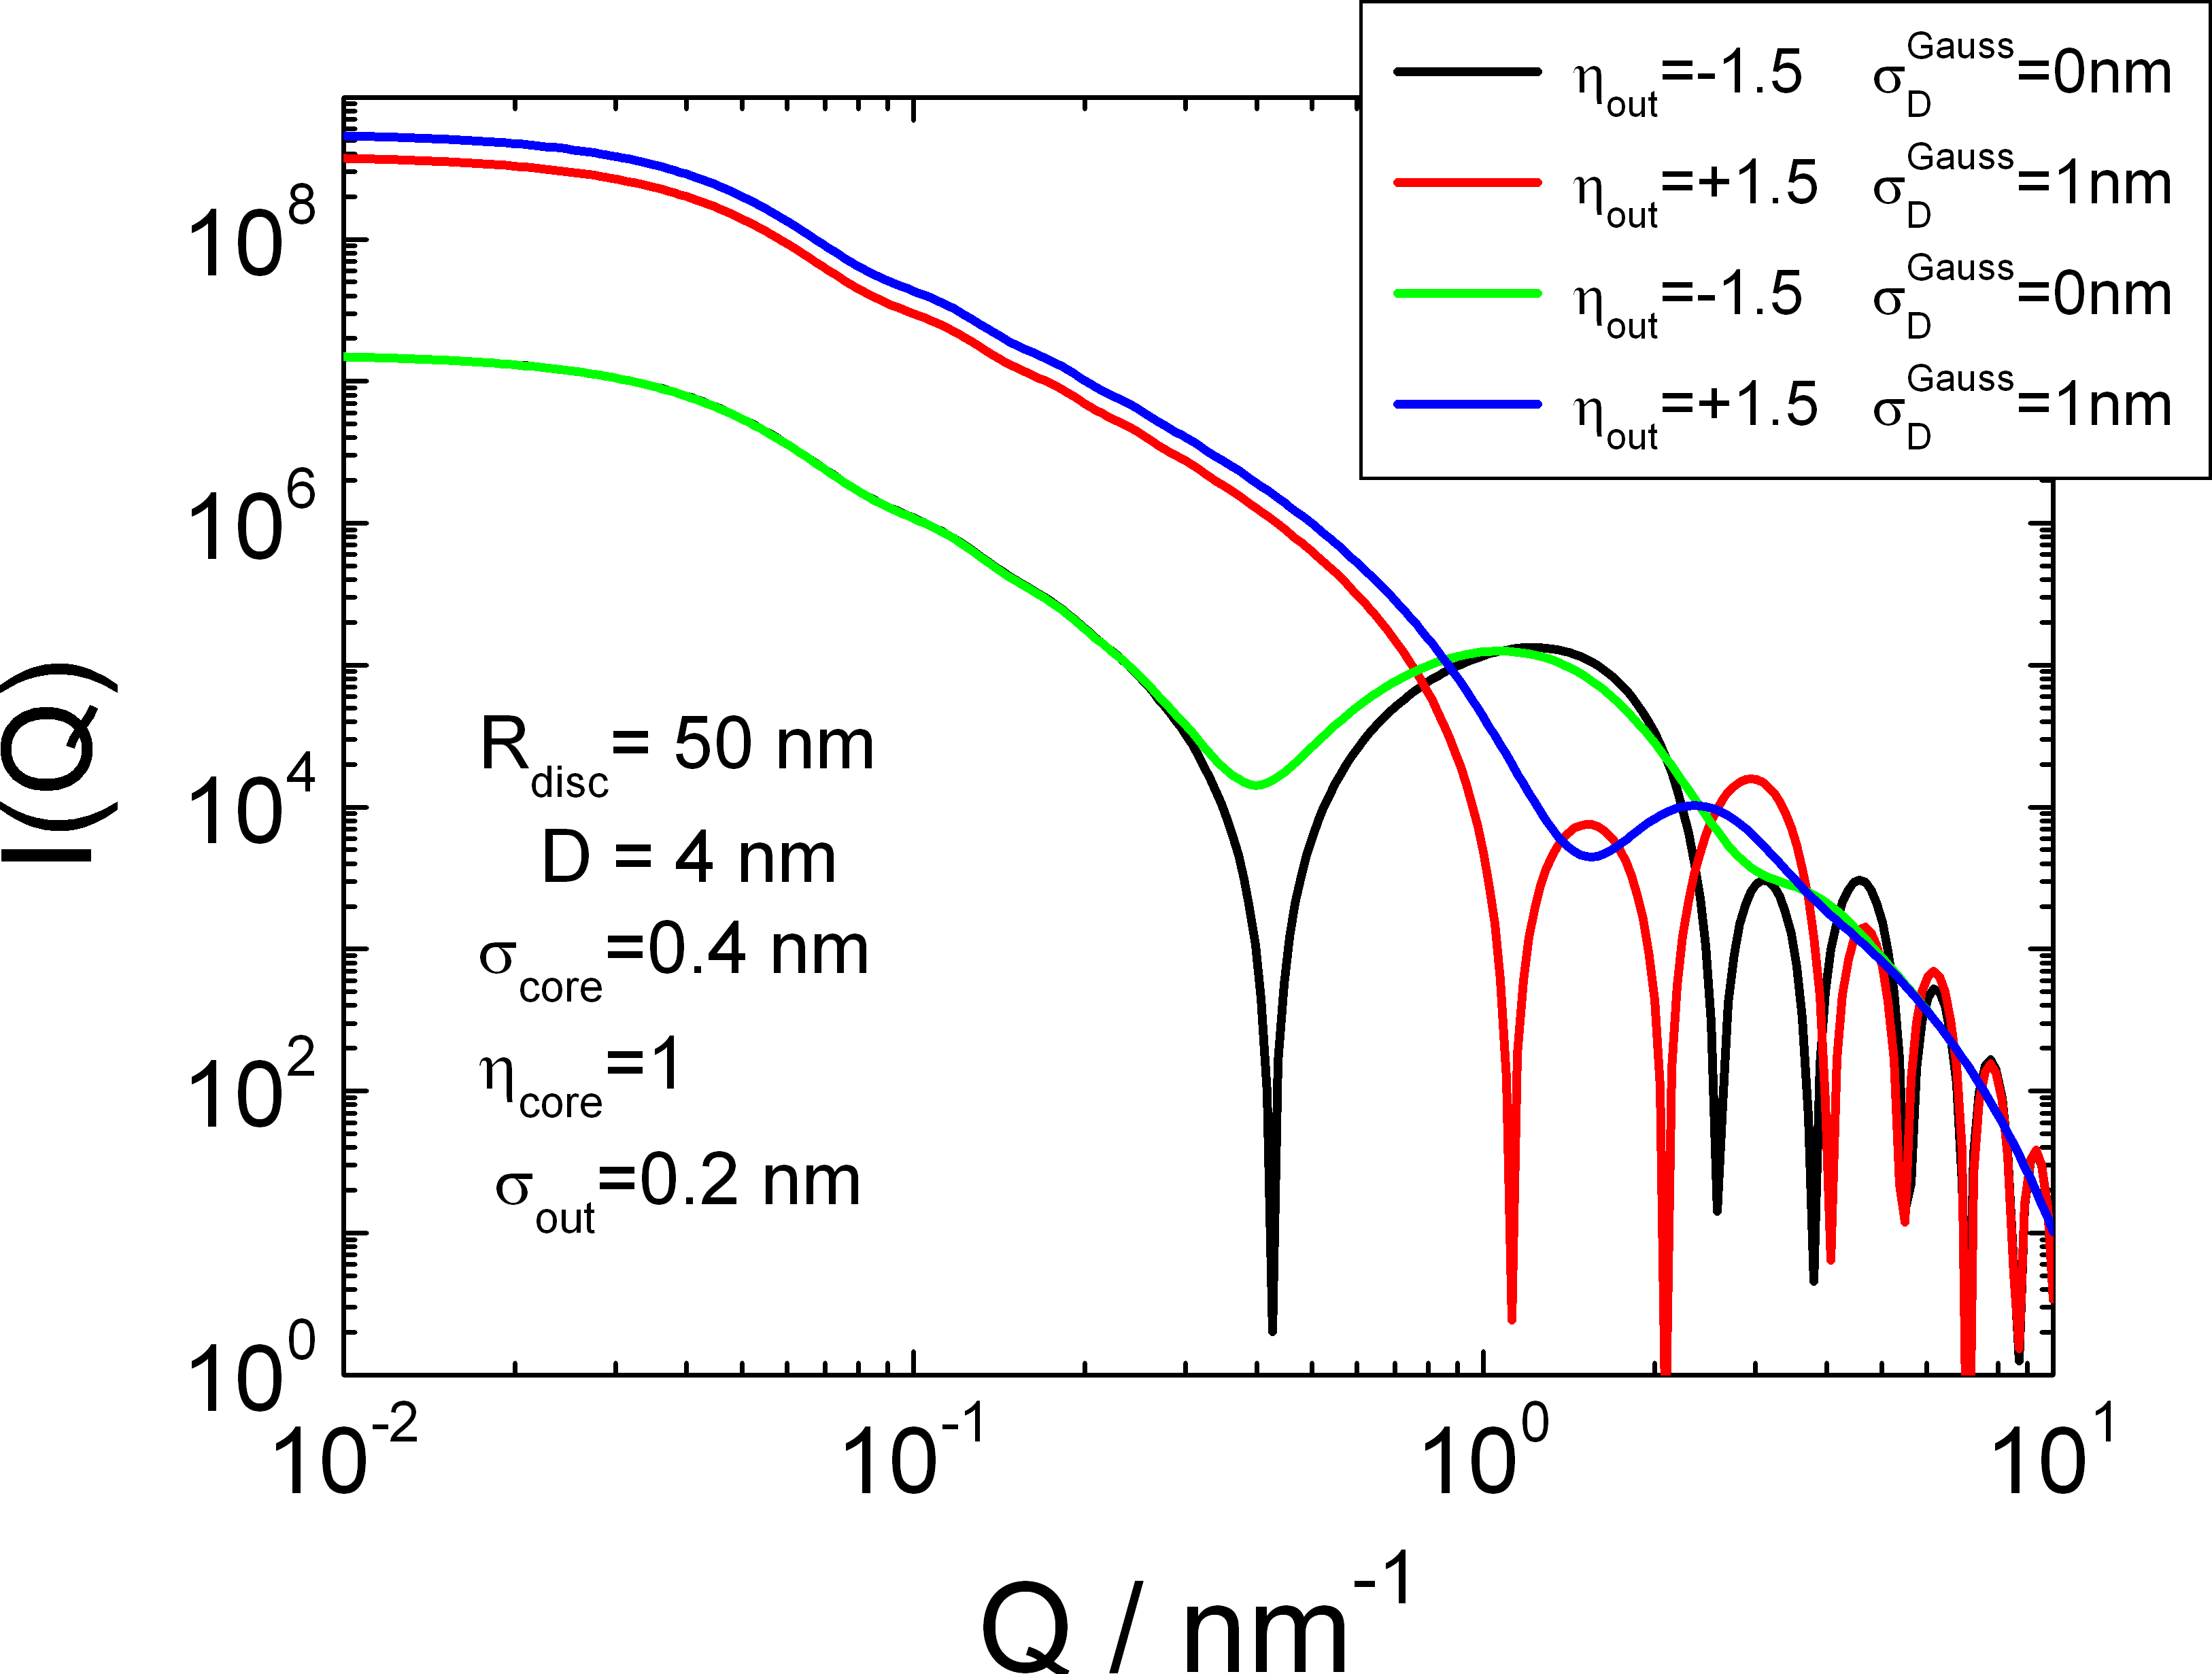
\includegraphics[width=0.48\textwidth,height=0.35\textwidth]{../images/form_factor/anisotropic/BiLayerGauss_IQa.png}}
\hfill
\subfigure[Plot of the cross section form factor $P_\text{cs}$ only according to eq.\ \ref{eq:PcsBilayer}.
The parameters for the profile are the same than in Fig.\ \ref{fig:BiLayerGaussianProfileIQ}a]{
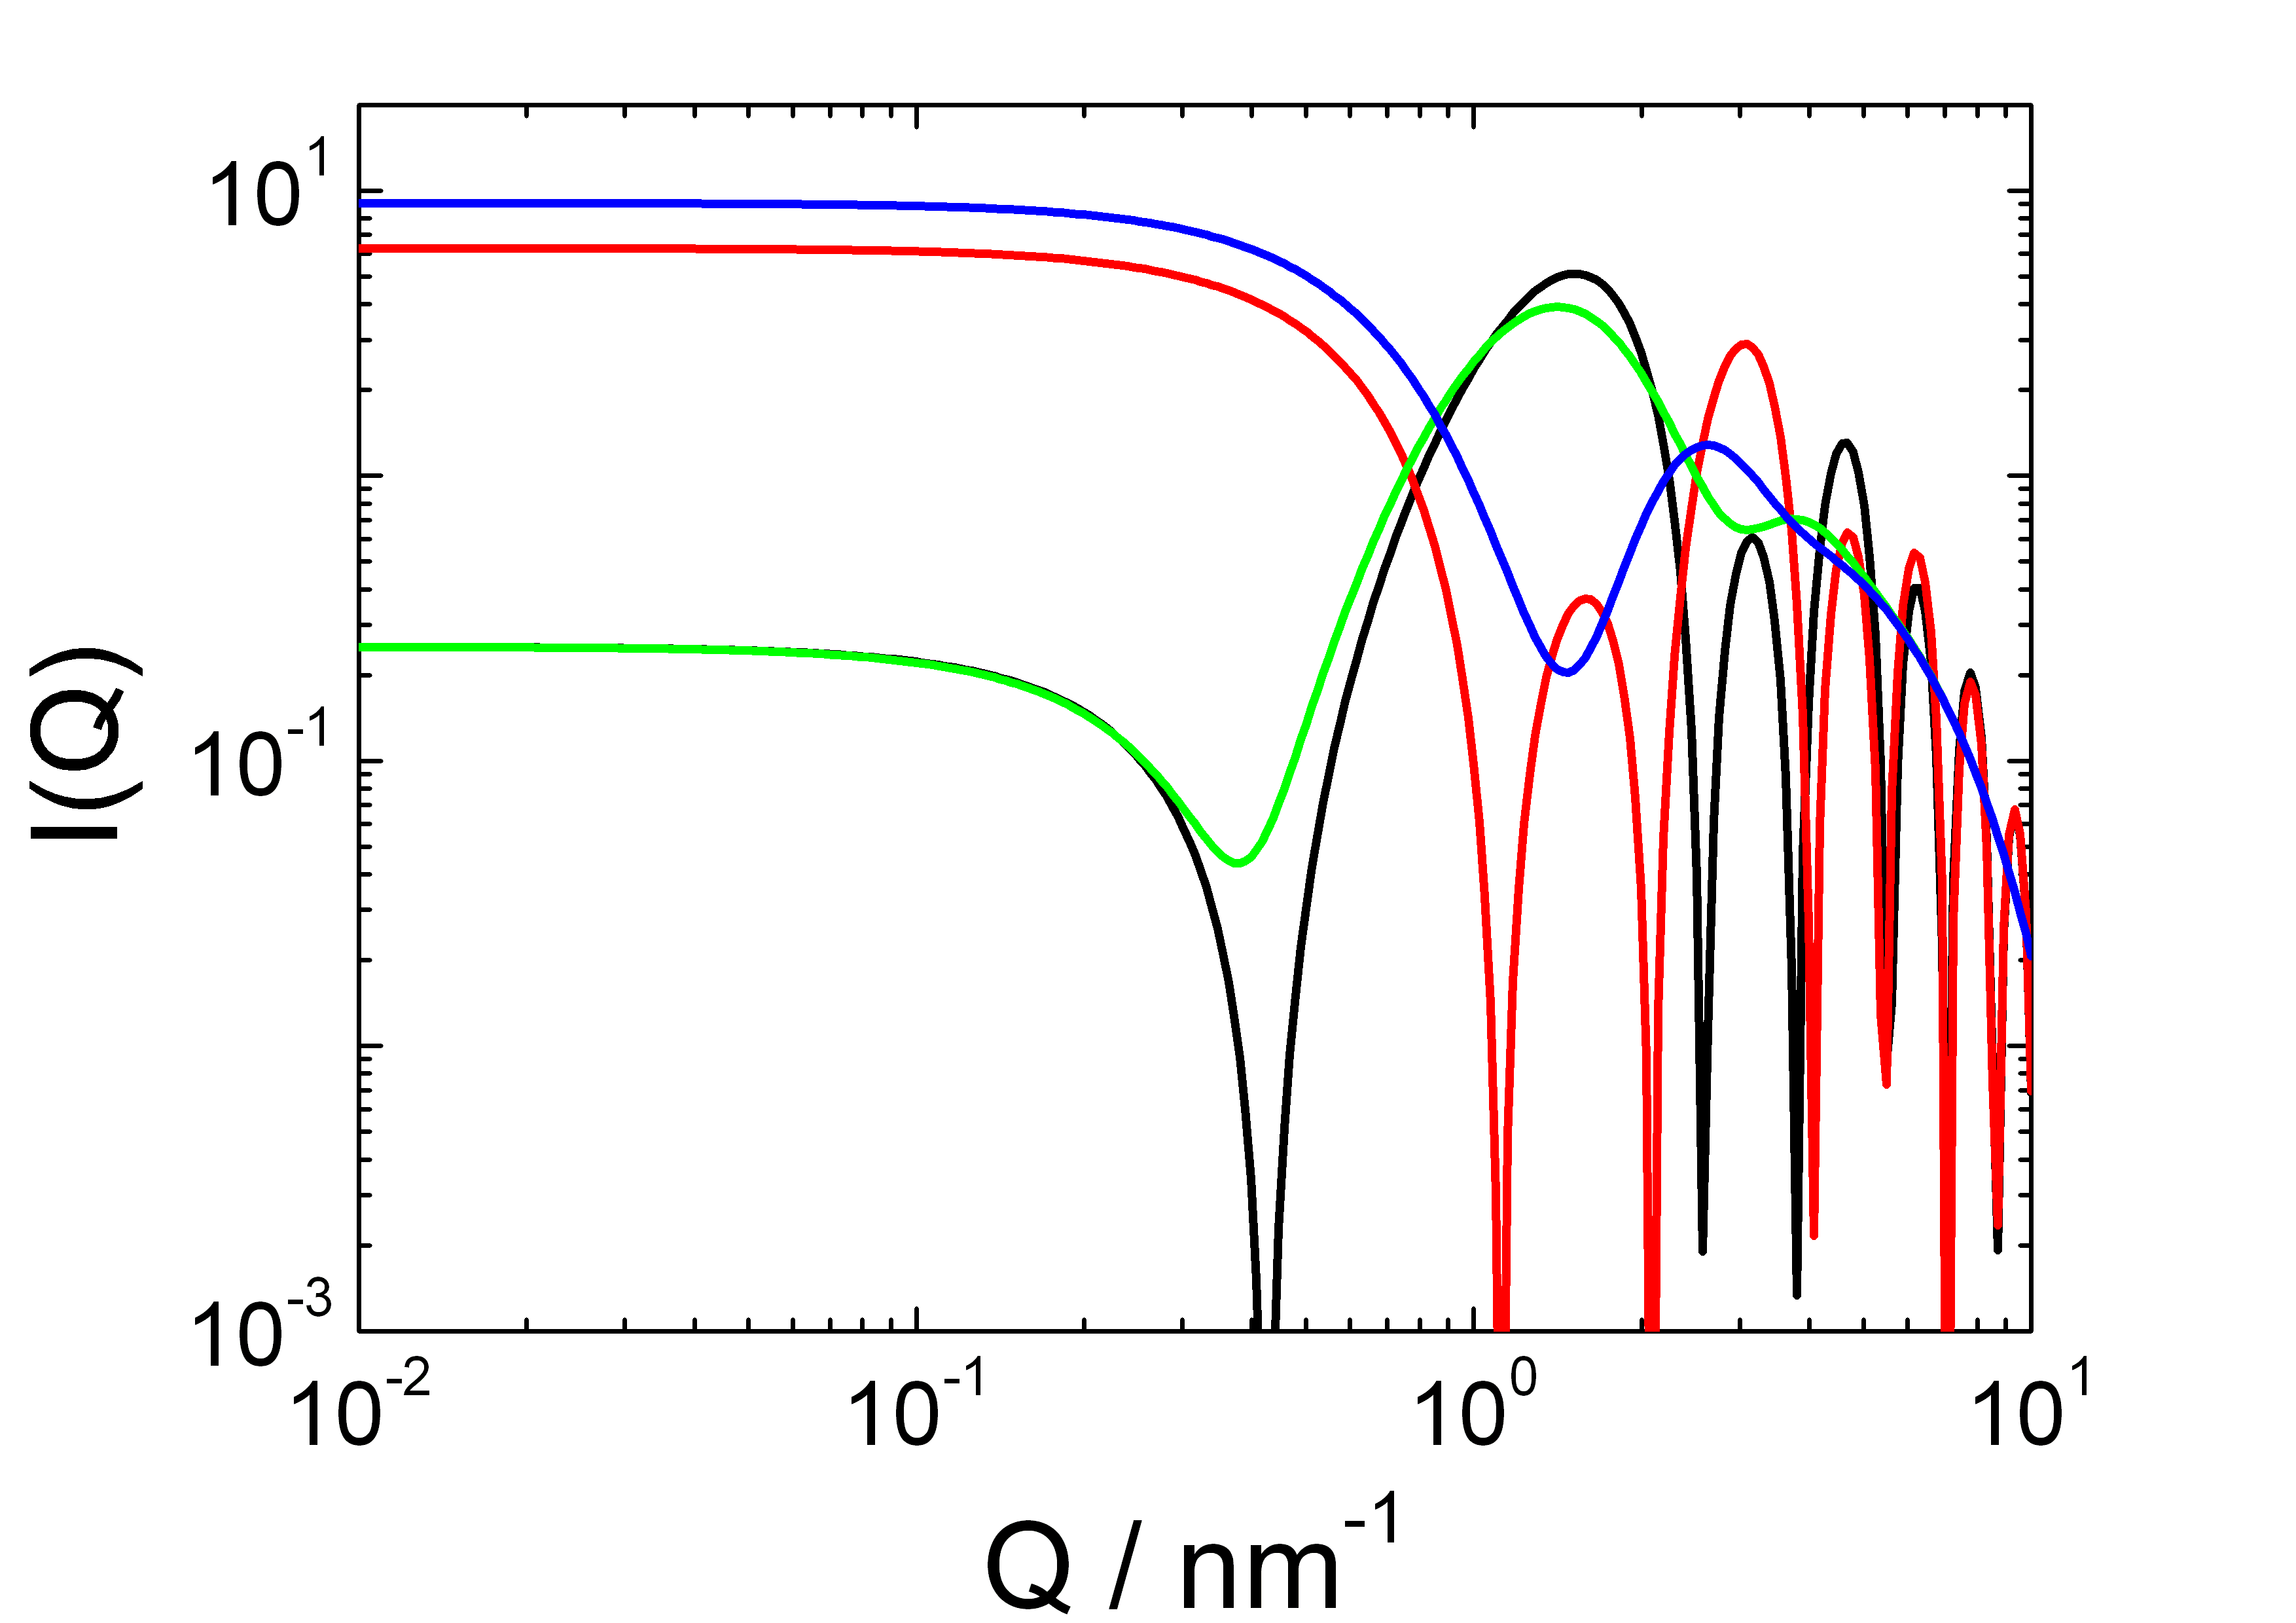
\includegraphics[width=0.48\textwidth,height=0.35\textwidth]{../images/form_factor/anisotropic/BiLayerGauss_IQb.png}}
\end{center}
\caption{Scattering curve for the cross-section form factor "\texttt{Pcs:BilayerGaussian}". For some of the curves a distance distribution of
the heads groups are assumed being Gaussian (see eq.\ \ref{eq:GaussDistribution}), i.e. calculating
$\int_0^\infty \mathrm{Gauss}(D,1,\sigma_D^\textrm{Gauss},D_0) P_\text{cs}\left(Q,D\right)\, \mathrm{d}D$.}
\label{fig:BiLayerGaussianProfileIQ}
\end{figure}


%
%\clearpage
%\subsubsection{Pcs(Q) for local planar objects with Gaussian chains attached to the  surface} ~\\
%\label{plugin:Pcs:GaussianChains}
%
%\begin{figure}[htb]
%\begin{center}
%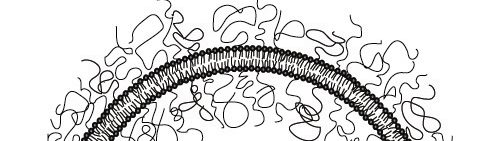
\includegraphics[width=0.962\textwidth,height=0.282\textwidth]{../images/form_factor/anisotropic/Plate+Chains(RW).png}
%\end{center}
%\caption{Sketch of a lipid bilayer with PEG molecules attached to them, which would be an example for local planar
%and objects with homogeneous core and Gaussian chains attached to the surface.}
%\label{fig:Plate+Chains(RW)}
%\end{figure}
%
%This cross-section form factor belongs to a whole class of form factors developed from
%Pedersen, Gerstenberg, and Svaneborg
%\cite{PedersenJApplCryst2000,PedersenGerstenberg96,SvaneborgPedersen2002,Richter1997}
%for self assembled block copolymers forming micelles of different shapes.
%They have assumed that one unit is forming the core of the
%micelles and the other the corona. The core is assumed to have a
%homogeneous scattering length density, but may contain some amount
%of solvent whereas the soluble blocks form a diffuse corona surrounding the core.
%
%The cross-section form factor of a micelle contains four different terms \cite{Pedersen2002}
%\begin{align}
%\begin{split}
%P_\text{cs}(Q)
% &=  \Bigg( r_\textrm{core}^2\,\left(\frac{\sin(QL/2)}{QL/2}\right)^2 + r_\textrm{brush} N_\text{agg} P_\text{brush}(Q)  \\
% & + N_\text{agg}(N_\text{agg}-1)r_\text{brush}^2\,S_\textrm{bb}(Q) + 2N_\text{agg} r_\text{core}r_\text{brush}\,S_\text{bc}(Q)\Bigg)
%\end{split}
%\end{align}
%where $N_\text{agg}$ is the total aggregation number of polymers on the surface, and
%$r_\text{brush}=V_\text{brush}(\eta_\text{brush}-\eta_\text{solv})$
%the excess scattering length of a single polymer chain in the corona
%and $r_\text{core}=V_\text{core}(\eta_\text{core}-\eta_\text{solv})$
%the total  excess scattering length of the core, respectively.
%$V_\text{brush}$ is the volume of a a single polymer chain in the corona
%and $V_\text{core}$ the total volume of the core. $\eta_\text{brush}$ and $\eta_\text{core}$ are the corresponding
%scattering length densities and $\eta_\text{solv}$ is the scattering length
%density of the surrounding solvent.
%
%The functions $P_\text{core}(Q)$, $P_\text{brush}(Q)$,
%$S_\text{bc}(Q)$, and $S_\text{bb}(Q)$ are all 1 for $q=0$.
%They are defined as
%
%\noindent
%\textbf{Input parameters for \texttt{Pcs:Plate+Chains(RW)}:}
%\begin{description}
%    \item[\texttt{L\_core}] thickness of the core of the planar layer $L_\textrm{core}$
%    \item[\texttt{n\_agg}] specific aggregation number $n_\textrm{agg}$ in units of number of chains per surface area
%    \item[\texttt{V\_brush}]  molecular volume of single chain in corona $V_\textrm{brush}$ in nm$^3$ for $Q$ in nm$^{-1}$
%                              or in \AA$^3$ for $Q$ in \AA$^{-1}$
%    \item[\texttt{eta\_core}] scattering length density of the core $\eta_\textrm{core}$
%    \item[\texttt{eta\_brush}] scattering length density of a Gaussian chain in corona $\eta_\textrm{brush}$
%    \item[\texttt{eta\_solv}] scattering length density of solvent $\eta_\textrm{solv}$
%    \item[\texttt{xsolv\_core}] amount of solvent in core $X_\textrm{xsolc,core}$
%    \item[\texttt{Rg}] gyration radius $R_G$ of polymer chains in the corona
%    \item[\texttt{d}] Value $d$ should be around 1.
%                      Non-penetration of the chains into the core is mimicked by $d\simeq 1$ for $L_\textrm{core} \gg R_G$
%\end{description}
%
%\noindent
%\textbf{Note}
%\begin{itemize}
%  \item This form factor is supposed to be combined with a shape factor for
%local planar objects which are implemented as structure  plugins
%under "\texttt{by plugin|anisotropic obj.|P'(Q): local planar
%obj.}".
%\end{itemize}
%
%\begin{figure}[htb]
%\begin{center}
%\subfigure[Plot of the cross section form factor $P_\text{cs}$ only according to eq.\ \ref{eq:PcsBilayer}.]{
%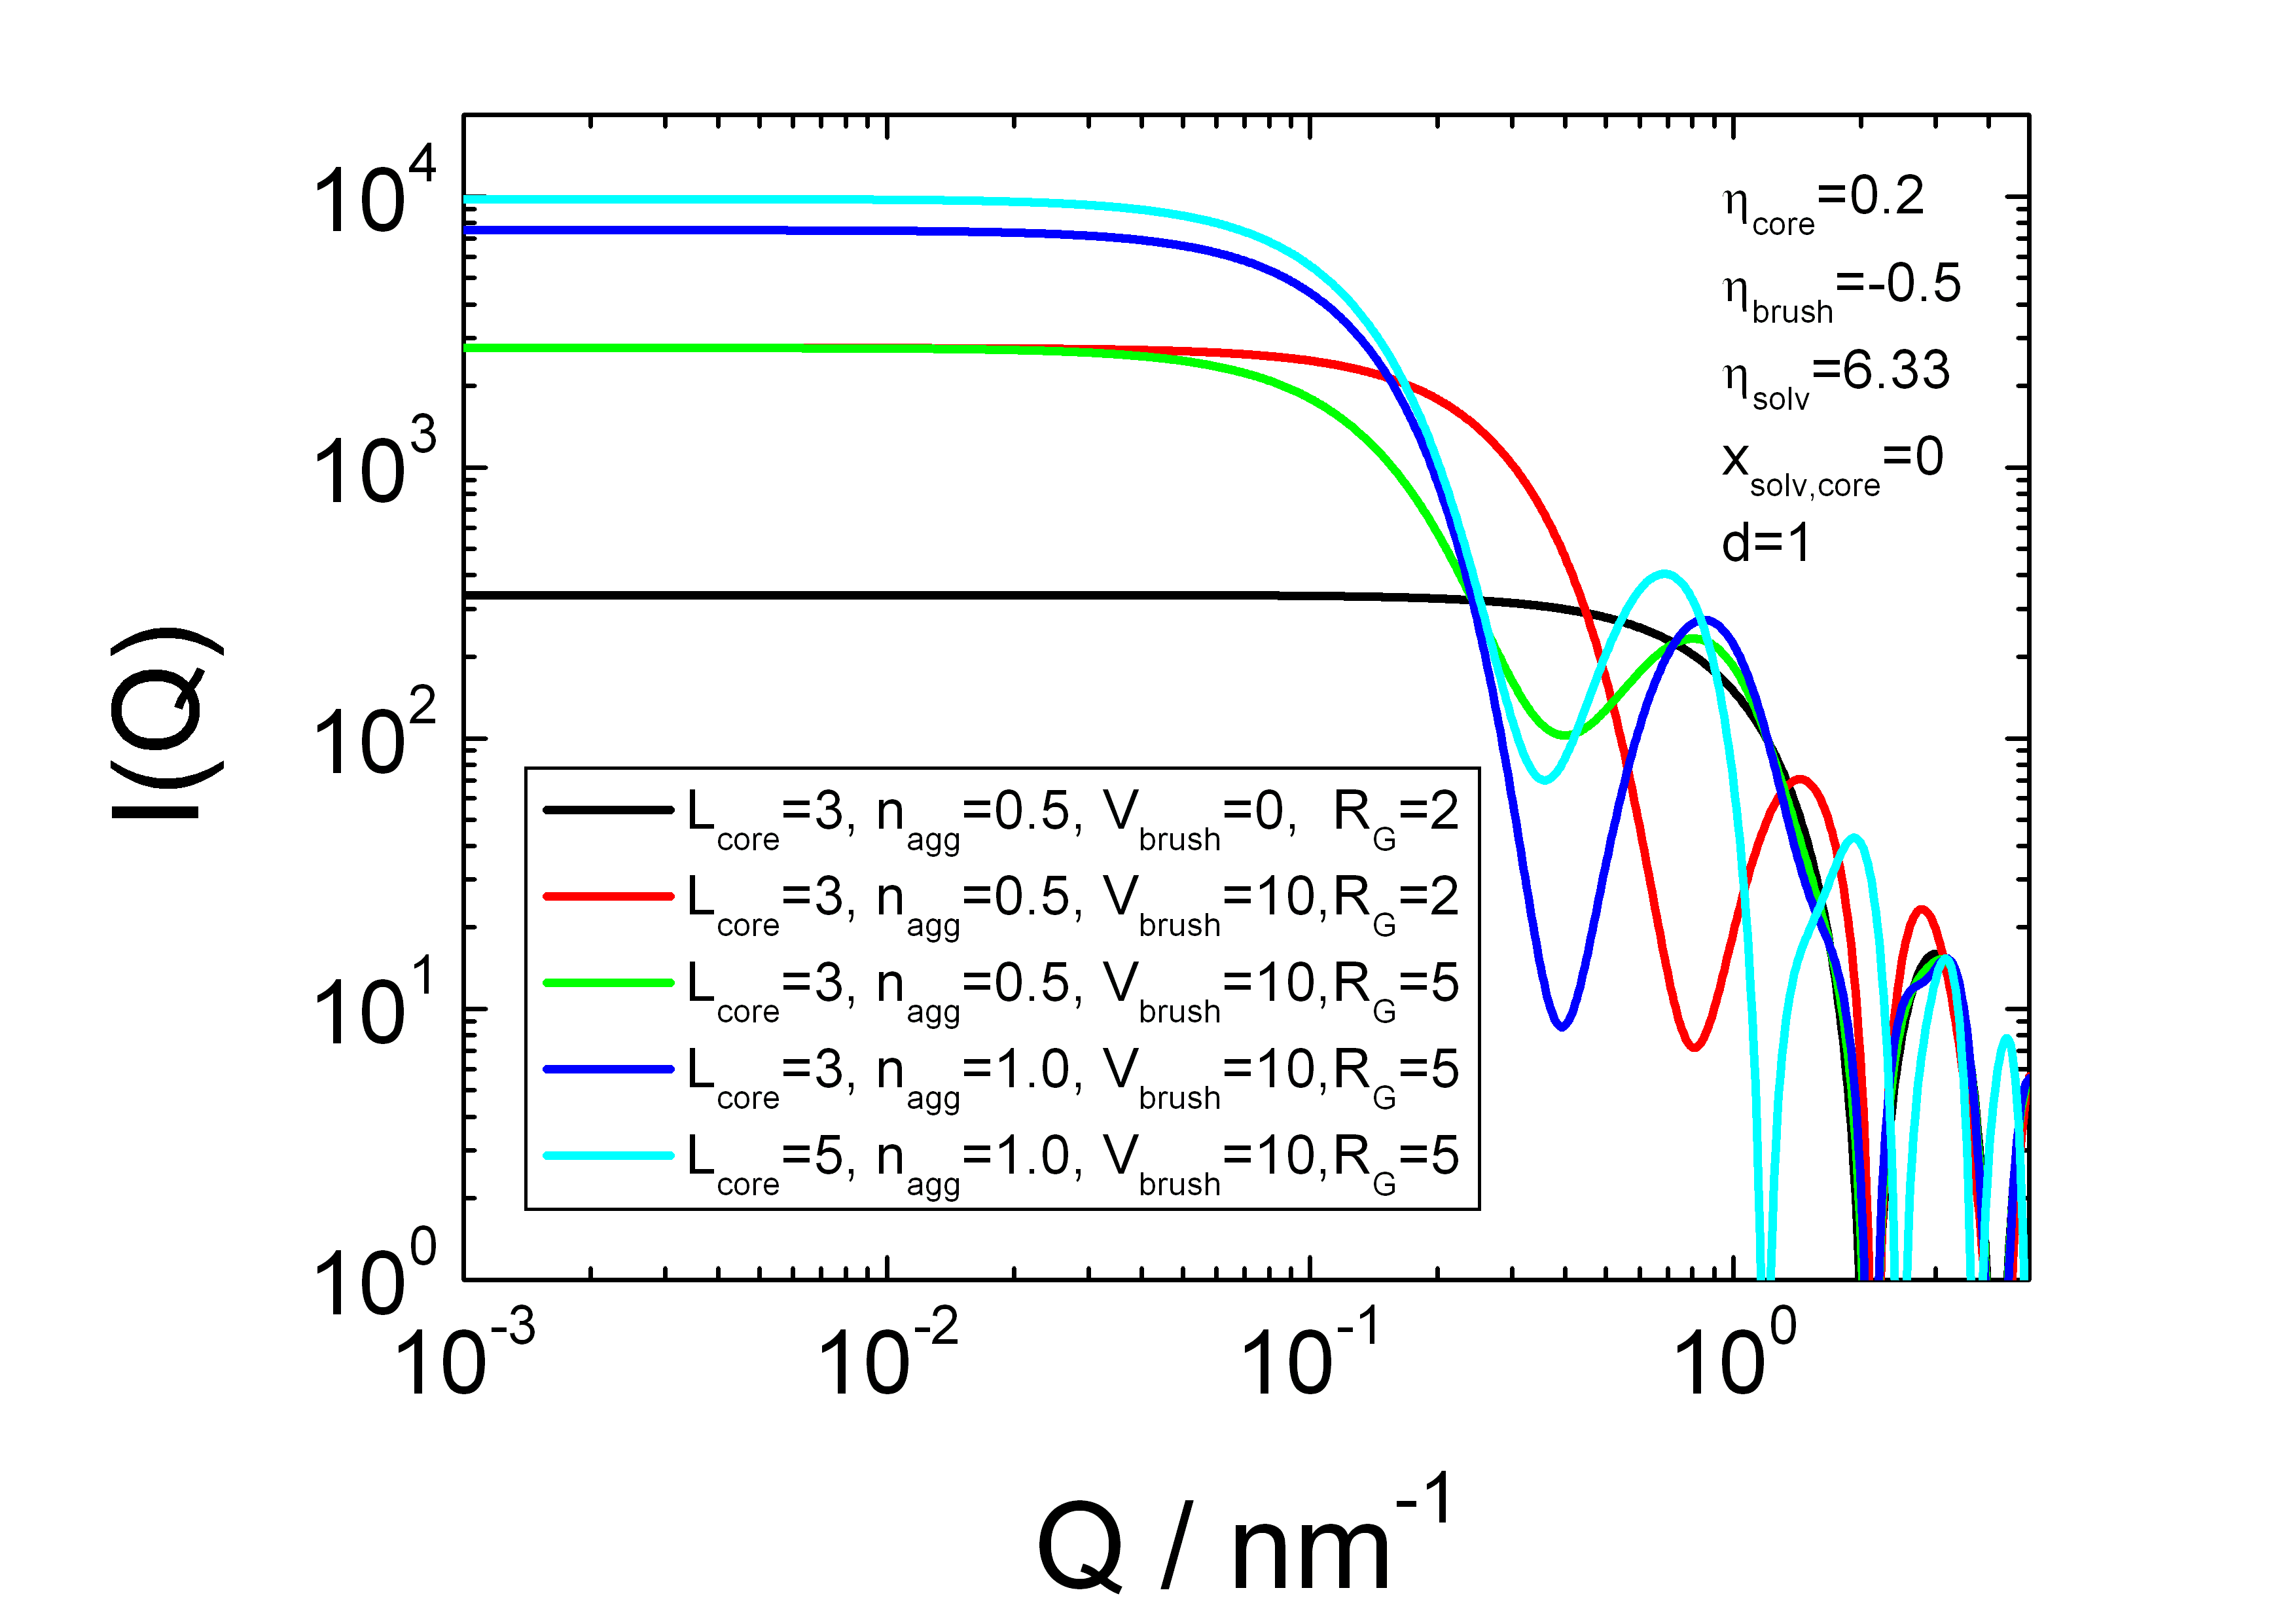
\includegraphics[width=0.48\textwidth,height=0.35\textwidth]{../images/form_factor/anisotropic/Pcs_Plate_Chains_RW_IQa.png}}
%\hfill
%\subfigure[Plot of the cross section form factor $P_\text{cs}$ in combination with a structure factor "\texttt{P'(Q): Thin Spherical Shell}"
%as the shape factor $P'(Q)$. The parameters for the profile are the same than in Fig.\ \ref{fig:Pcs_Plate_Chains_RW_IQ}a]{
%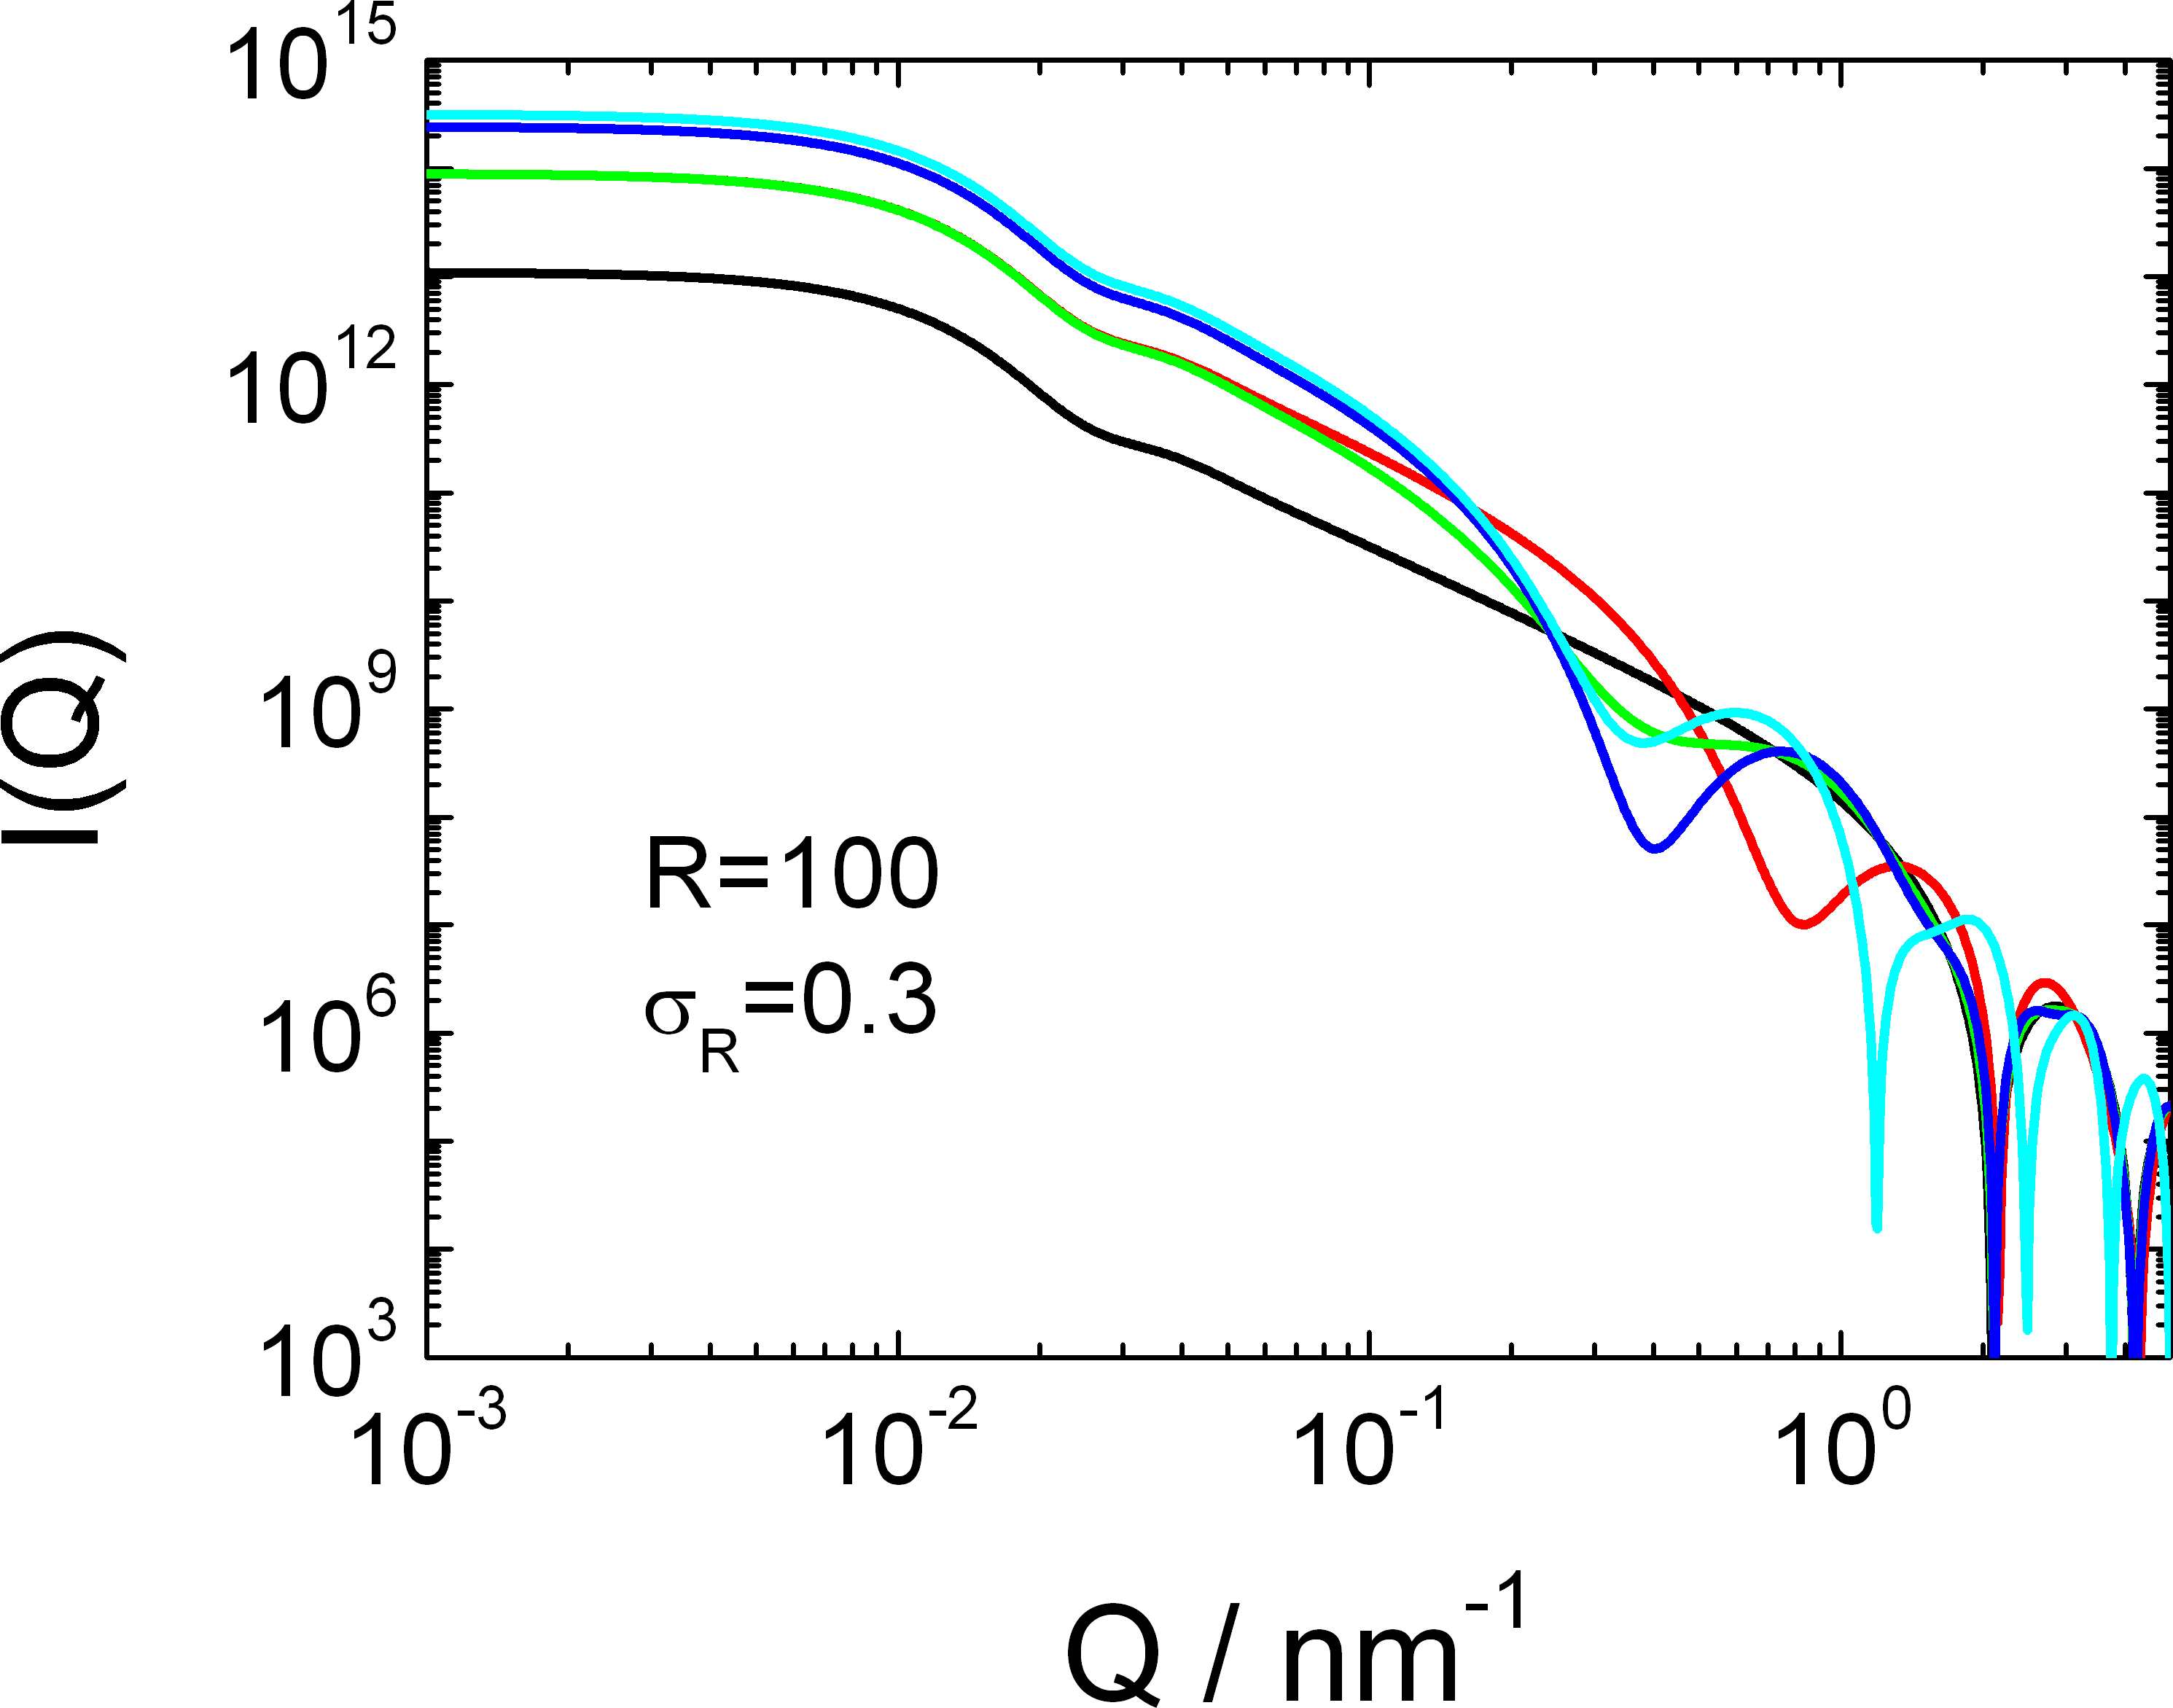
\includegraphics[width=0.48\textwidth,height=0.35\textwidth]{../images/form_factor/anisotropic/Pcs_Plate_Chains_RW_IQb.png}}
%\end{center}
%\caption{Scattering curves for the cross-section form factor "\texttt{Pcs:Plate+Chains(RW)}".}
%\label{fig:Pcs_Plate_Chains_RW_IQ}
%\end{figure}

\clearpage
\subsection{Pcs(Q) for cylindrical obj.} ~\\
\label{plugin:Pcs4cylindrical}

The cross-section form factors with cylindrical geometry are valid
when the cross-section dimension is much smaller than the segment length
or Kuhn length of the local cylindrical structure.

\begin{figure}[htb]
  % Requires \usepackage{graphicx}
  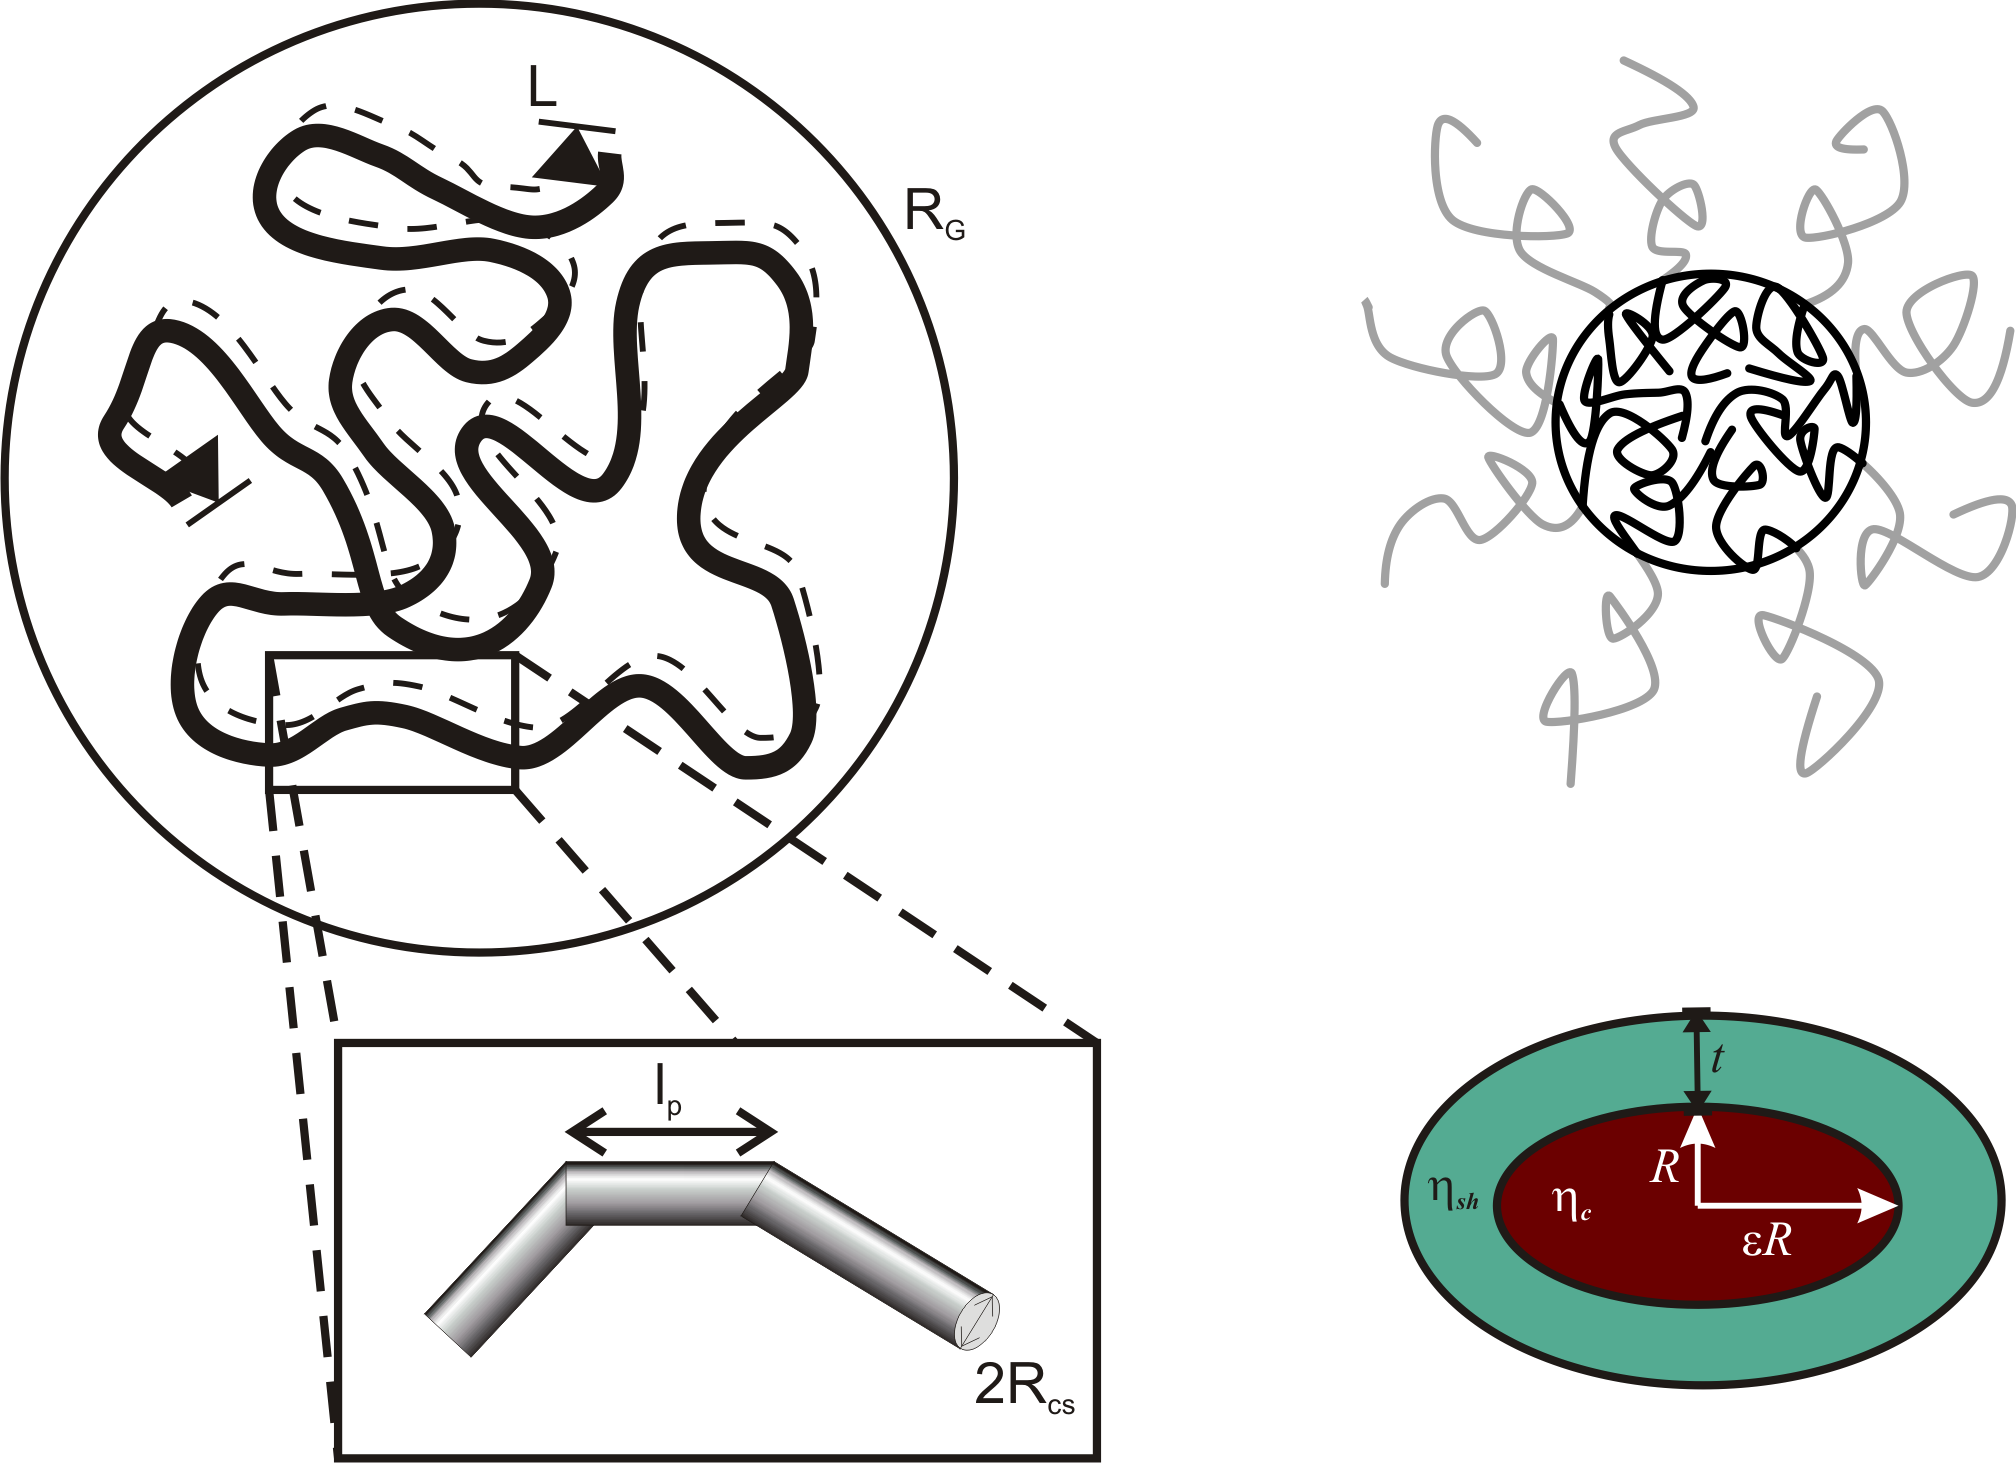
\includegraphics[width=0.85\textwidth]{../images/form_factor/anisotropic/SketchdiffXSWorm.png}\\
  \caption{Sketch of wormlike structures which represent local cylindrical structures. The cross-section $2R_\text{cs}$
  is much smaller than the Kuhn length $l_p$, which is a typical length scale where a freely jointed chain can randomly orient
  in any direction without the influence of any forces, independent of the directions taken by other segments.
  For the cross-section term several profiles have been implemented, like homogeneous round profile or elliptical shell profile}\label{fig:WormSketchdiffXS}
\end{figure}


\clearpage
\subsubsection{Pcs(Q) for homogeneous cross-section of a cylinder} ~\\
\label{plugin:Pcs:homogeneousXS_cyl}


This cross-section form factor describes the scattering of circular and homogeneous cross section.
The cross-section radius $R$ can have a distribution described by a log-normal distribution according
to eq.\ \ref{eq:LogNormal}.

\begin{align}
P_\text{cs}(Q,\sigma_{R},R) = \int_0^\infty \textrm{LogNorm}(x,1,\sigma_{R},1,R) \left( \left(\eta_\textrm{core}-\eta_\textrm{solv}\right) \pi x^2 \frac{2 \mathrm{J}_1(Qx)}{Qx} \right)^2 \, \textrm{d}x
\end{align}

\noindent
\textbf{Input parameters for \texttt{Pcs:homogeneousCyl}:}
\begin{description}
    \item[\texttt{R}] most probable radius $R$
    \item[\texttt{sigm\_R}] width $\sigma_R$ of radius distribution (LogNorm)
    \item[\texttt{dummy}] not used
    \item[\texttt{dummy}] not used
    \item[\texttt{dummy}] not used
    \item[\texttt{dummy}] not used
    \item[\texttt{dummy}] not used
    \item[\texttt{eta\_core}] scattering length density of the core $\eta_\textrm{core}$
    \item[\texttt{dummy}] not used
    \item[\texttt{eta\_solv}] scattering length density of the solvent $\eta_\textrm{solv}$
\end{description}

\noindent
\textbf{Note}
\begin{itemize}
  \item This form factor is supposed to be combined with a shape factor for
local cylindrical objects which are implemented as structure  plugins
under "\texttt{[by plugin|anisotropic obj.|P'(Q): local cylindrical obj.]}".
\item As the form factor already have the width distribution included one normally uses in \SASfit as a size distribution
the \texttt{Delta}-distribution.
\end{itemize}

\begin{figure}[htb]
\begin{center}
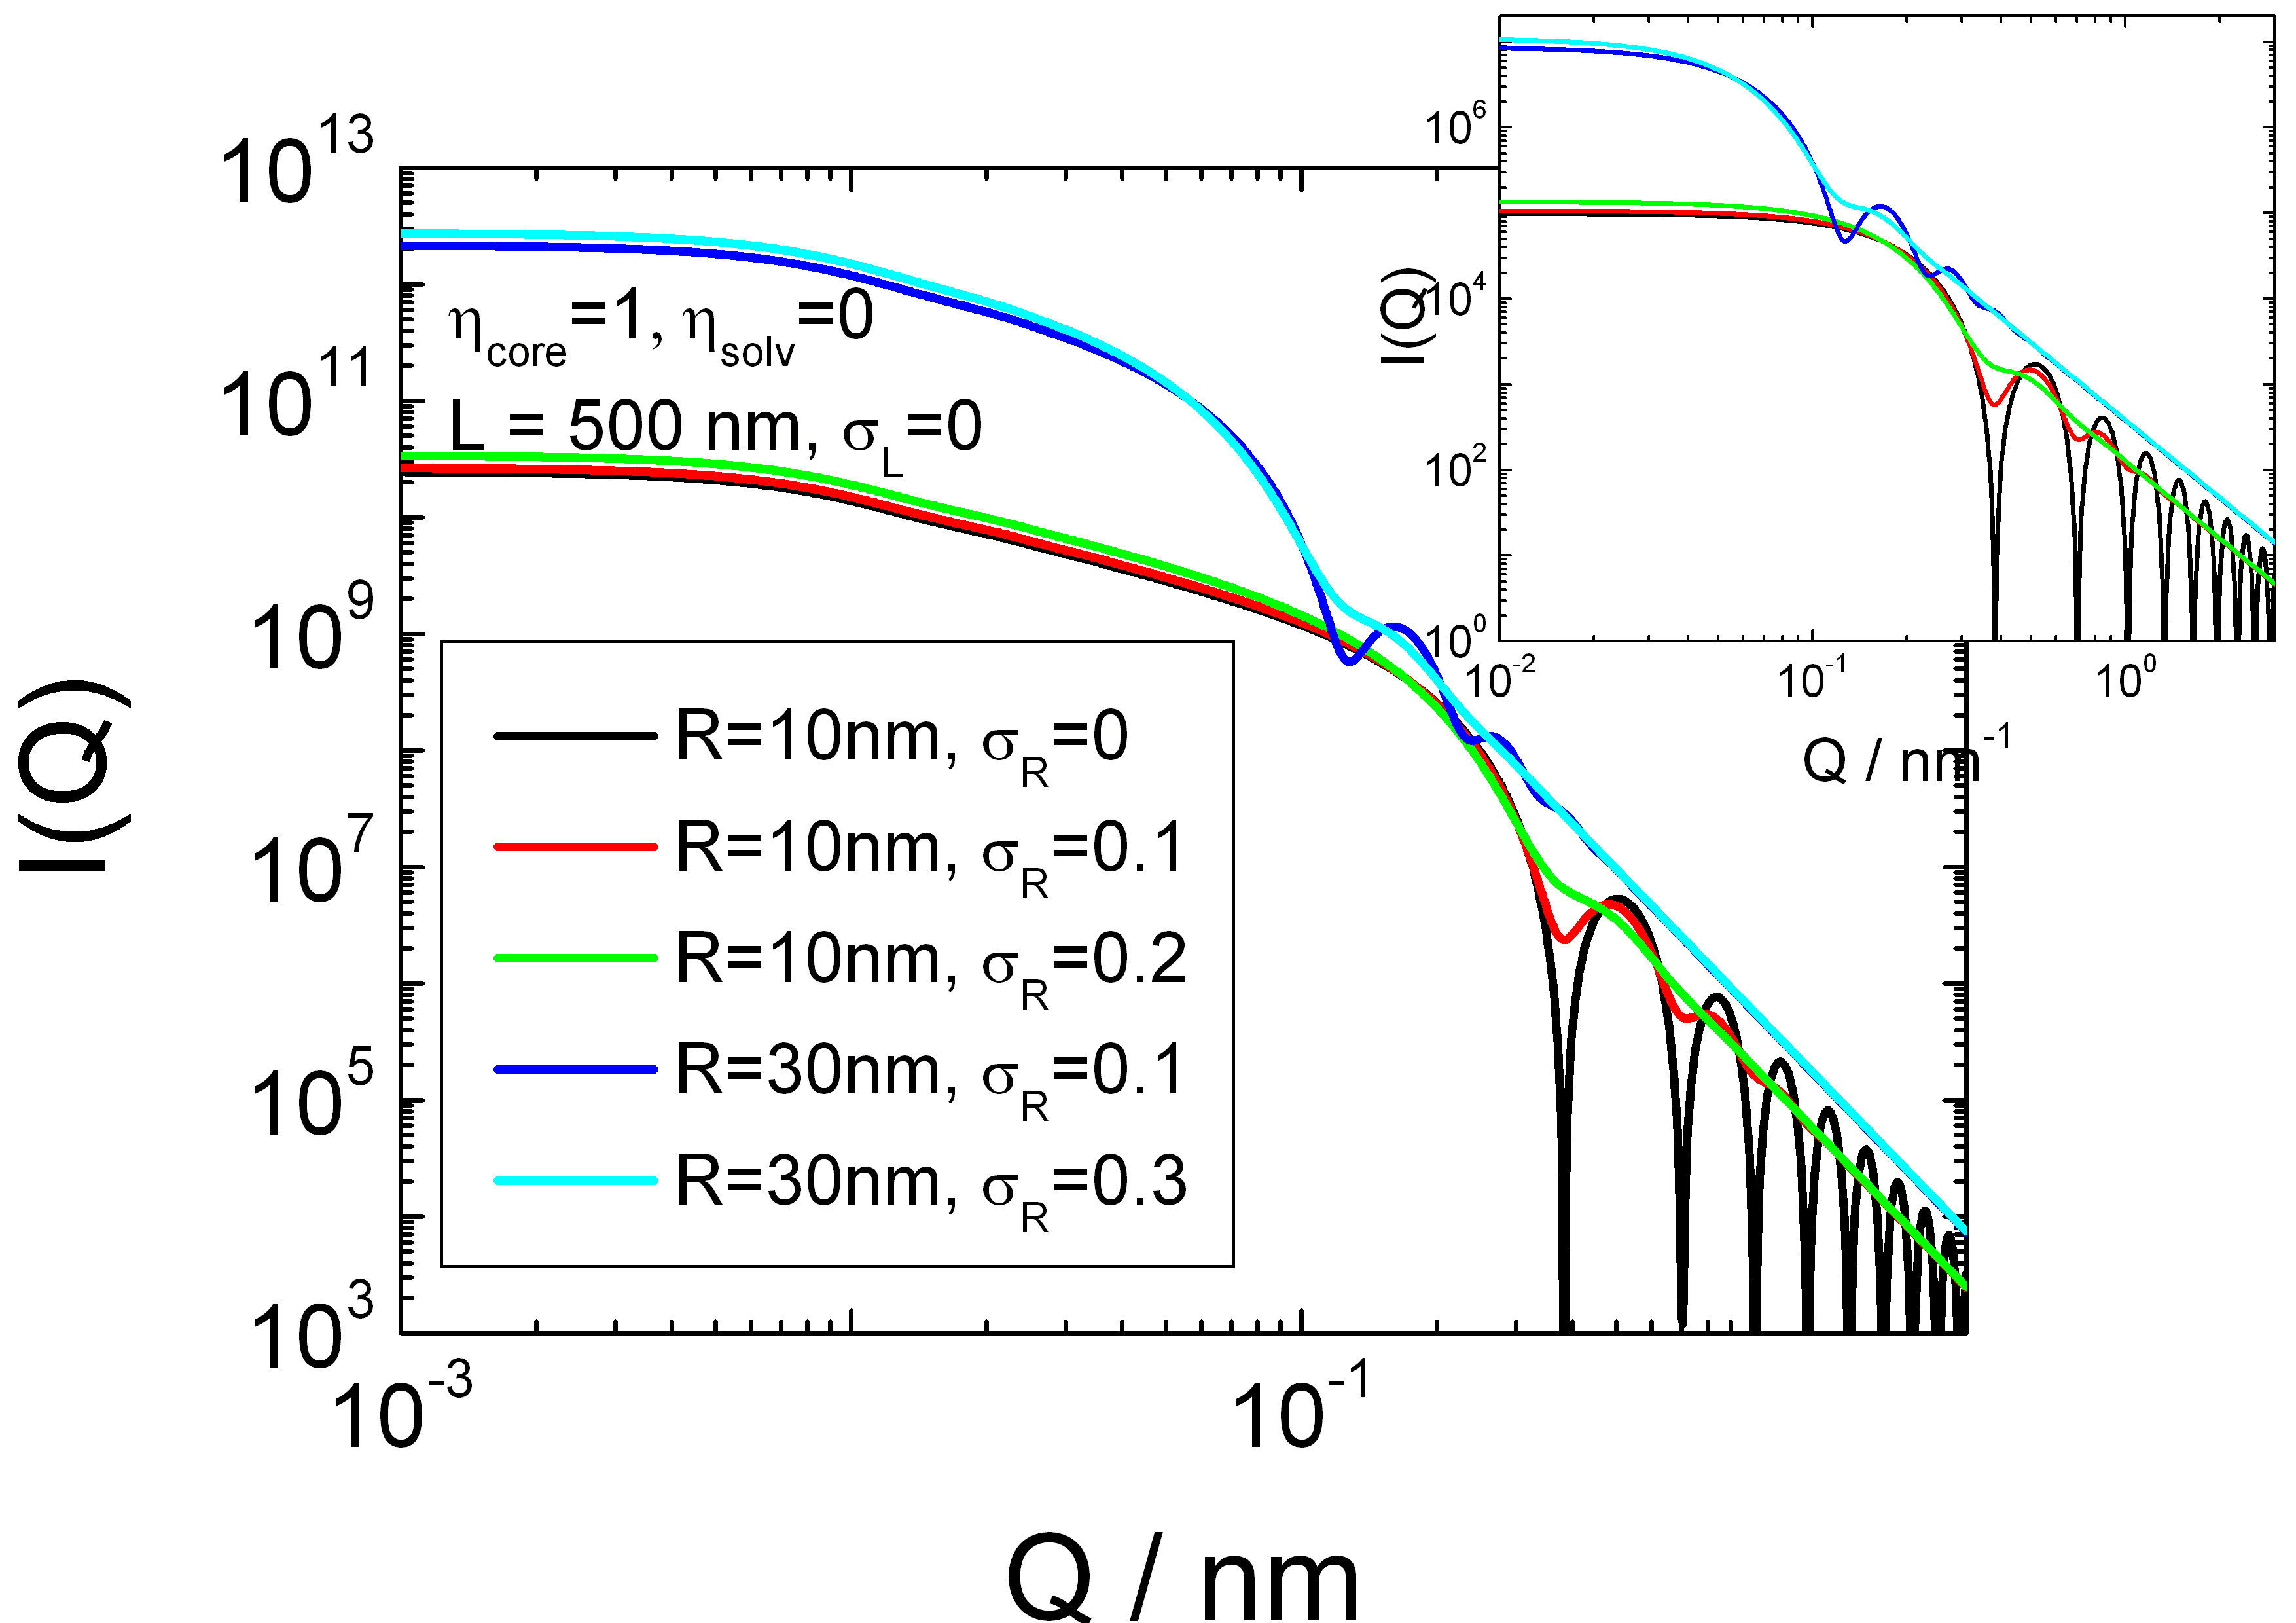
\includegraphics[width=0.8\textwidth,height=0.55\textwidth]{../images/form_factor/anisotropic/CylindricalHomogeneousXSIQ.png}
\end{center}
\caption{Scattering curve for the form factor "\texttt{Pcs:homogeneousCyl}" only (insert) and
in combination with a structure factor "\texttt{P'(Q): Thin Rod}".}
\label{fig_IQ:Pcs:CylindricalHomogeneousXSIQ}
\end{figure}

\clearpage
\subsubsection{Pcs(Q) for cross-section of a cylindrical shell with elliptical cross section} ~\\
\label{plugin:Pcs:CylEllSh}

\noindent
This cross-section form factor describes the scattering of an elliptical core-shell cross-section.
The cross-section radius $R$ can have a distribution with a width of $sigma$ as
described by a log-normal distribution according to eq.\ \ref{eq:LogNormal}.

\begin{equation}
\begin{split}
    P_\textrm{cs}(Q) = & \int_0^\infty \textrm{LogNorm}(x,1,\sigma_{R},1,R)  \quad \times\\
        & \int_0^{\pi/2}
\Big[\left( \eta_\textrm{shell}-\eta_\textrm{solv}\right)F_\textrm{cs,ell}(Q,R+t,\epsilon,\phi) \\
& \quad + \left(\eta_\textrm{core}-\eta_\textrm{shell}\right)F_\textrm{cs,ell}(Q,R,\epsilon,\phi)
\Big]^2 \, \mathrm{d}\phi
\end{split}
\end{equation}
with
\begin{subeqnarray}
F_\textrm{cs,ell}\left(Q,R,\epsilon,\Delta\eta\phi\right) &=&  \frac{2 \mathrm{J}_1(Qr(R,\epsilon,\phi))}{Qr(R,\epsilon,\phi)}   \\
r(R,\epsilon,\phi) &=& R\sqrt{\sin^2\phi+\epsilon^2\cos^2\phi}
\end{subeqnarray}



\noindent
\textbf{Input parameters for \texttt{Pcs:homogeneousCyl}:}
\begin{description}
    \item[\texttt{R}] most probable radius $R$
    \item[\texttt{sigm\_R}] width $\sigma_R$ of radius distribution (LogNorm)
    \item[\texttt{epsilon}] eccentricity $\epsilon$ of ellipyical cross-section
    \item[\texttt{t}] shell thickness $t$
    \item[\texttt{dummy}] not used
    \item[\texttt{dummy}] not used
    \item[\texttt{dummy}] not used
    \item[\texttt{eta\_core}] scattering length density of the core $\eta_\textrm{core}$
    \item[\texttt{eta\_shell}] scattering length density of the shell $\eta_\textrm{shell}$
    \item[\texttt{eta\_solv}] scattering length density of the solvent $\eta_\textrm{solv}$
\end{description}

\noindent
\textbf{Note}
\begin{itemize}
  \item This form factor is supposed to be combined with a shape factor for
local cylindrical objects which are implemented as structure  plugins
under "\texttt{[by plugin|anisotropic obj.|P'(Q): local cylindrical obj.]}".
\item As the form factor already has the width distribution included one normally uses in \SASfit as a size distribution
the \texttt{Delta}-distribution.
\end{itemize}

\clearpage
\subsection{P'(Q) for local planar obj.} ~\\
\label{plugin:Pprime4planar}



\clearpage
\subsubsection{P'(Q): thin discs} ~\\
\label{plugin:Pprime4Discs}

\begin{figure}[htb]
\begin{center}
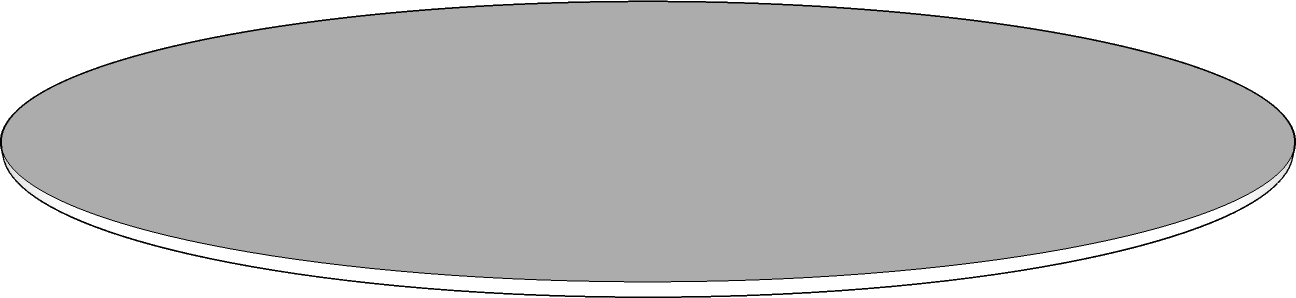
\includegraphics[width=0.686\textwidth,height=0.27\textwidth]{../images/form_factor/anisotropic/ThinDisc.png}
\end{center}
\caption{Sketch of a thin disc with a radius $R$. The thickness of the disc is assumed to be much smaller than its radius.}
\label{fig:ThinDisc}
\end{figure}

\noindent
\textbf{Input parameters for \texttt{P'(Q): Thin Disc}:}
\begin{description}
    \item[\texttt{R}] most probable radius $R$
    \item[\texttt{dummy}] not used
    \item[\texttt{sima}] width $\sigma$ of radius distribution (LogNorm)
\end{description}

\noindent
\textbf{Note}
\begin{itemize}
  \item This structure factor is supposed to be combined with a form factor of local planar objects which are implemented as form factor plugins
under "\texttt{[by plugin|anisotropic obj.|Pcs(Q): local planar obj.]}".
\item The structure factor already has a log-normal width distribution for one parameter included.
\end{itemize}

\begin{figure}[htb]
\begin{center}
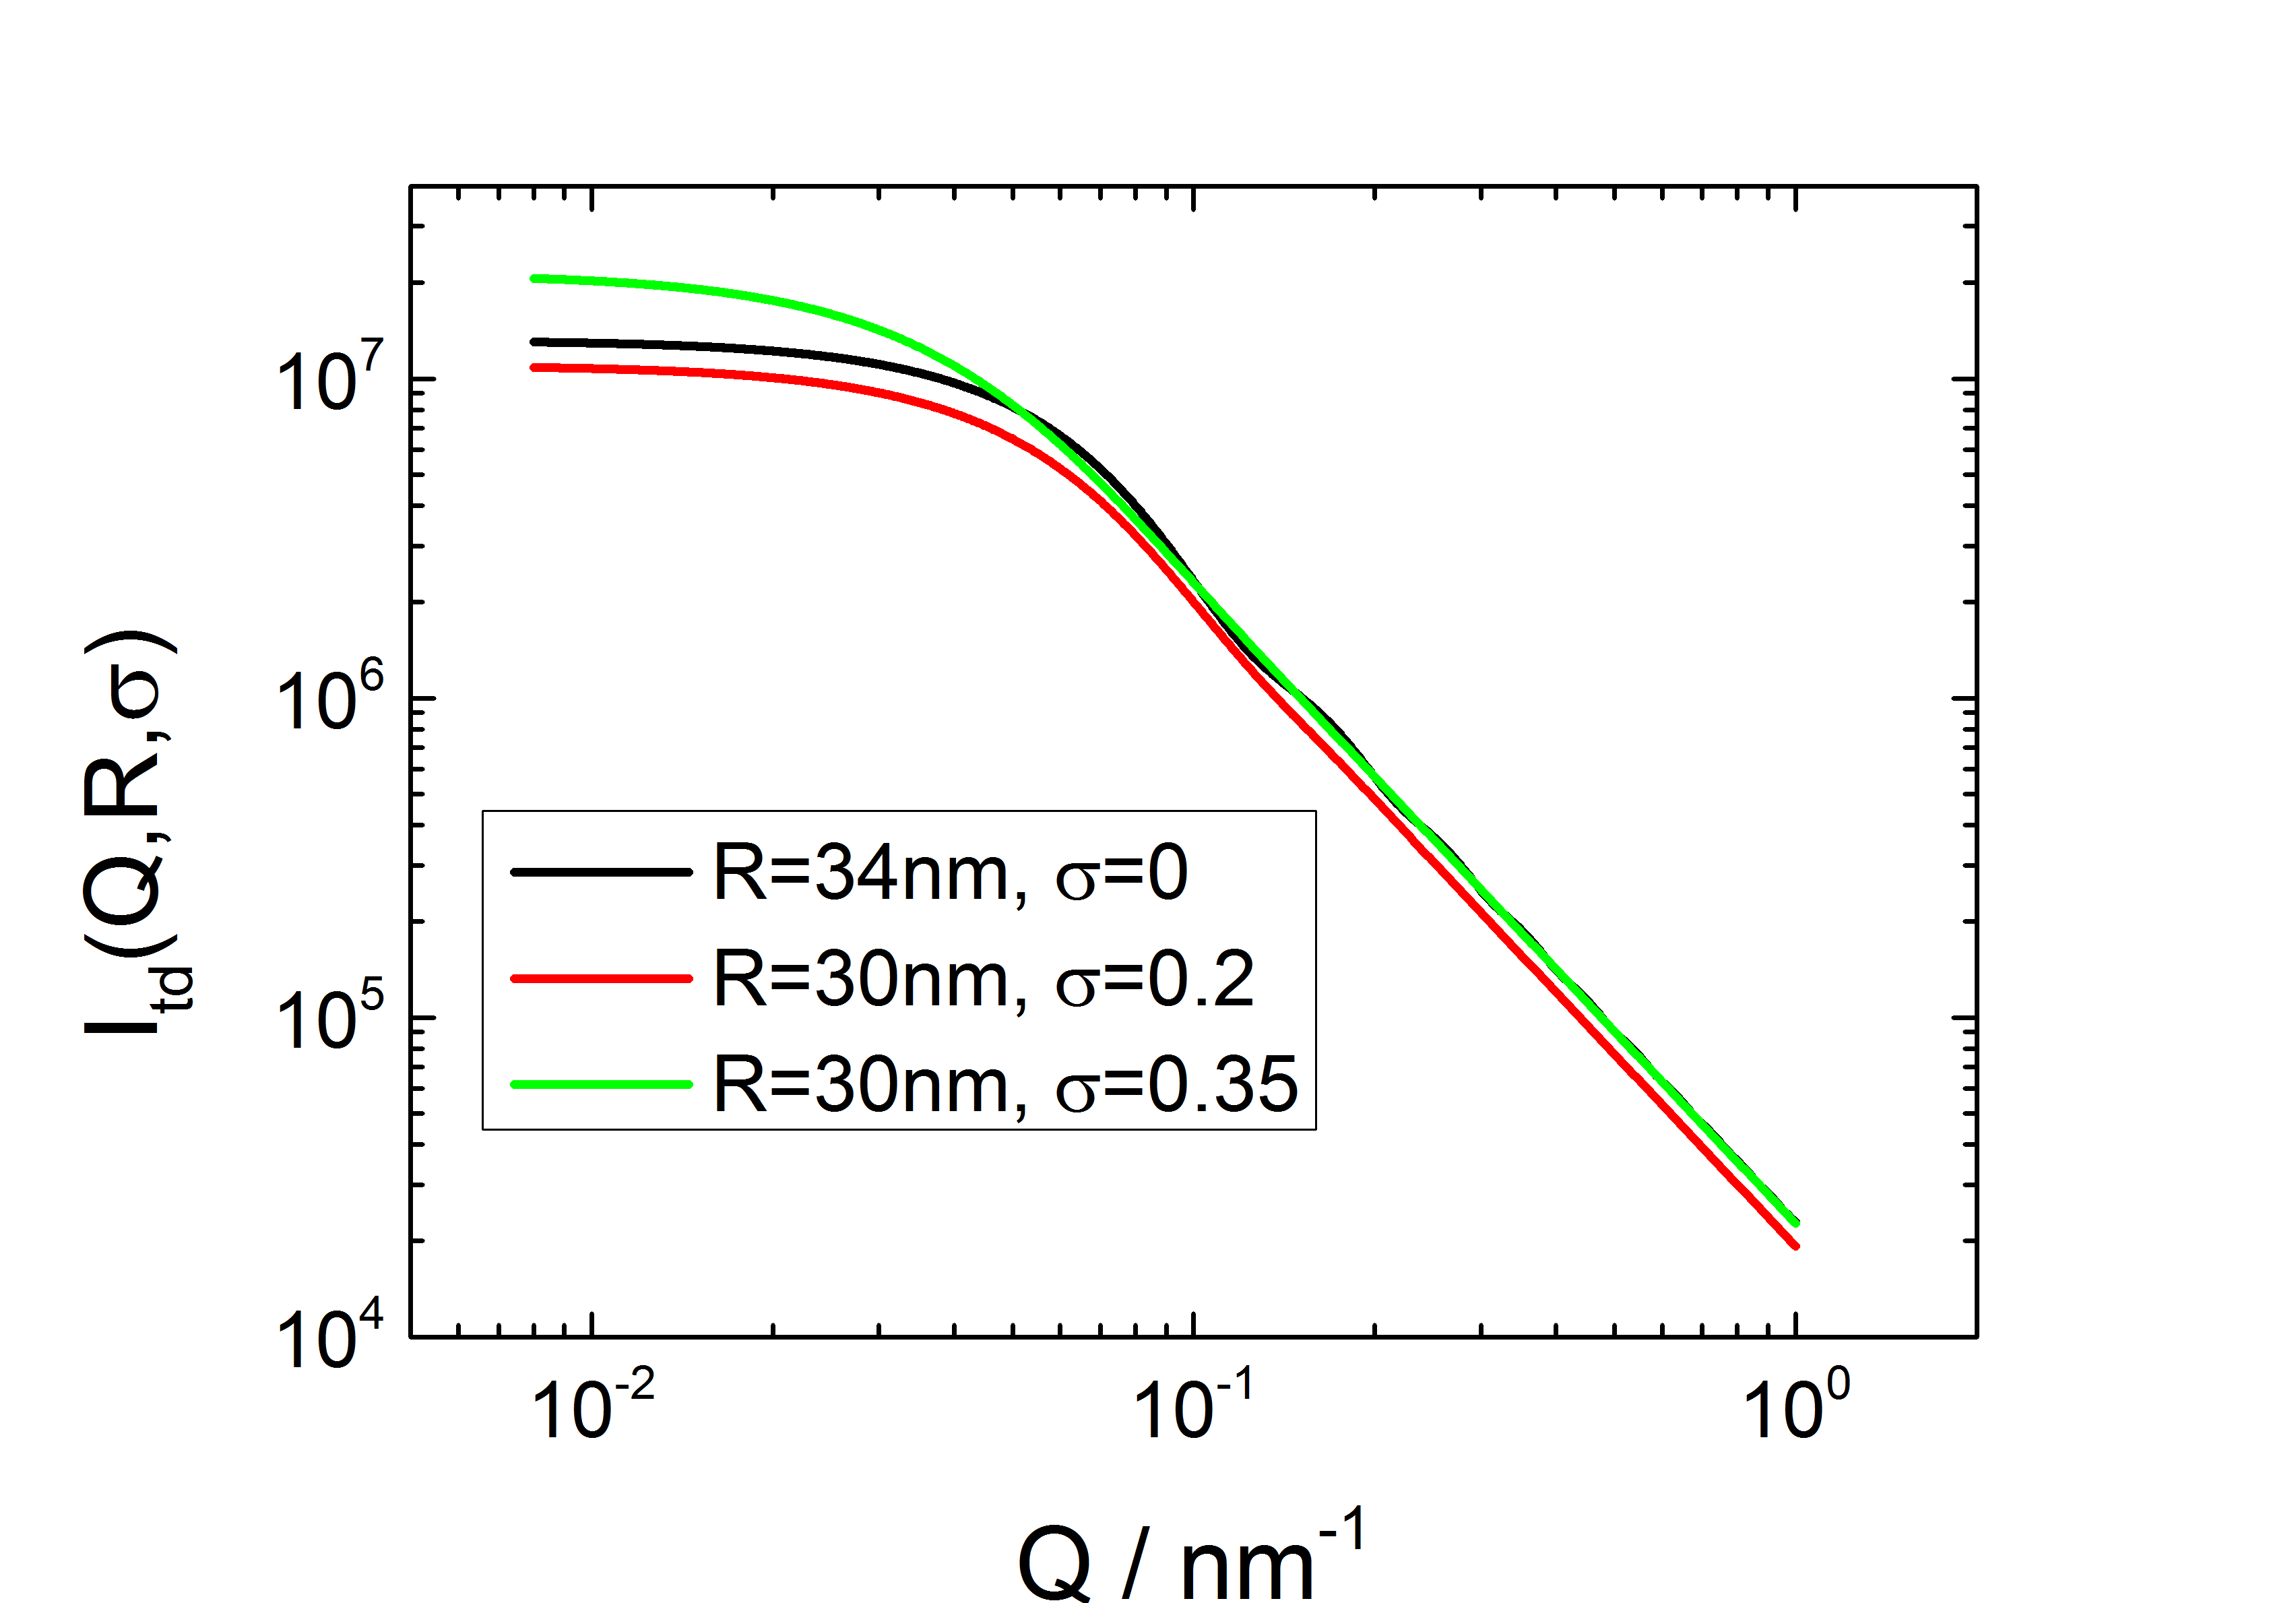
\includegraphics[width=0.8\textwidth,height=0.55\textwidth]{../images/form_factor/anisotropic/PprimeThinDisc.png}
\end{center}
\caption{Scattering curve for the structure factor "\texttt{P'(Q): Thin Disc}" in combination with a constant background of 1".}
\label{fig_IQ:PprimeThinDisc}
\end{figure}

\clearpage
\subsubsection{P'(Q): thin spherical shell} ~\\
\label{plugin:Pprime4spShell}

\begin{figure}[htb]
\begin{center}
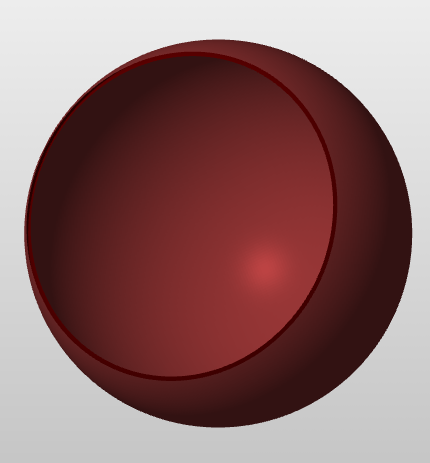
\includegraphics[width=0.43\textwidth,height=0.463\textwidth]{../images/form_factor/anisotropic/Sphere_thin.png}
\end{center}
\caption{Sketch of a thin spherical shell with a radius $R$. The thickness of the shell is assumed to be much smaller than the radius of the sphere.}
\label{fig:ThinSphericalShell}
\end{figure}

\noindent
\textbf{Input parameters for \texttt{P'(Q): Thin Spherical Shell}:}
\begin{description}
    \item[\texttt{R}] most probable radius $R$
    \item[\texttt{dummy}] not used
    \item[\texttt{sima}] width $\sigma$ of radius distribution (LogNorm)
\end{description}

\noindent
\textbf{Note}
\begin{itemize}
  \item This structure factor is supposed to be combined with a form factor of local planar objects which are implemented as form factor plugins
under "\texttt{[by plugin|anisotropic obj.|Pcs(Q): local planar obj.]}".
\item The structure factor already has a log-normal width distribution for one parameter included.
\end{itemize}

\begin{figure}[htb]
\begin{center}
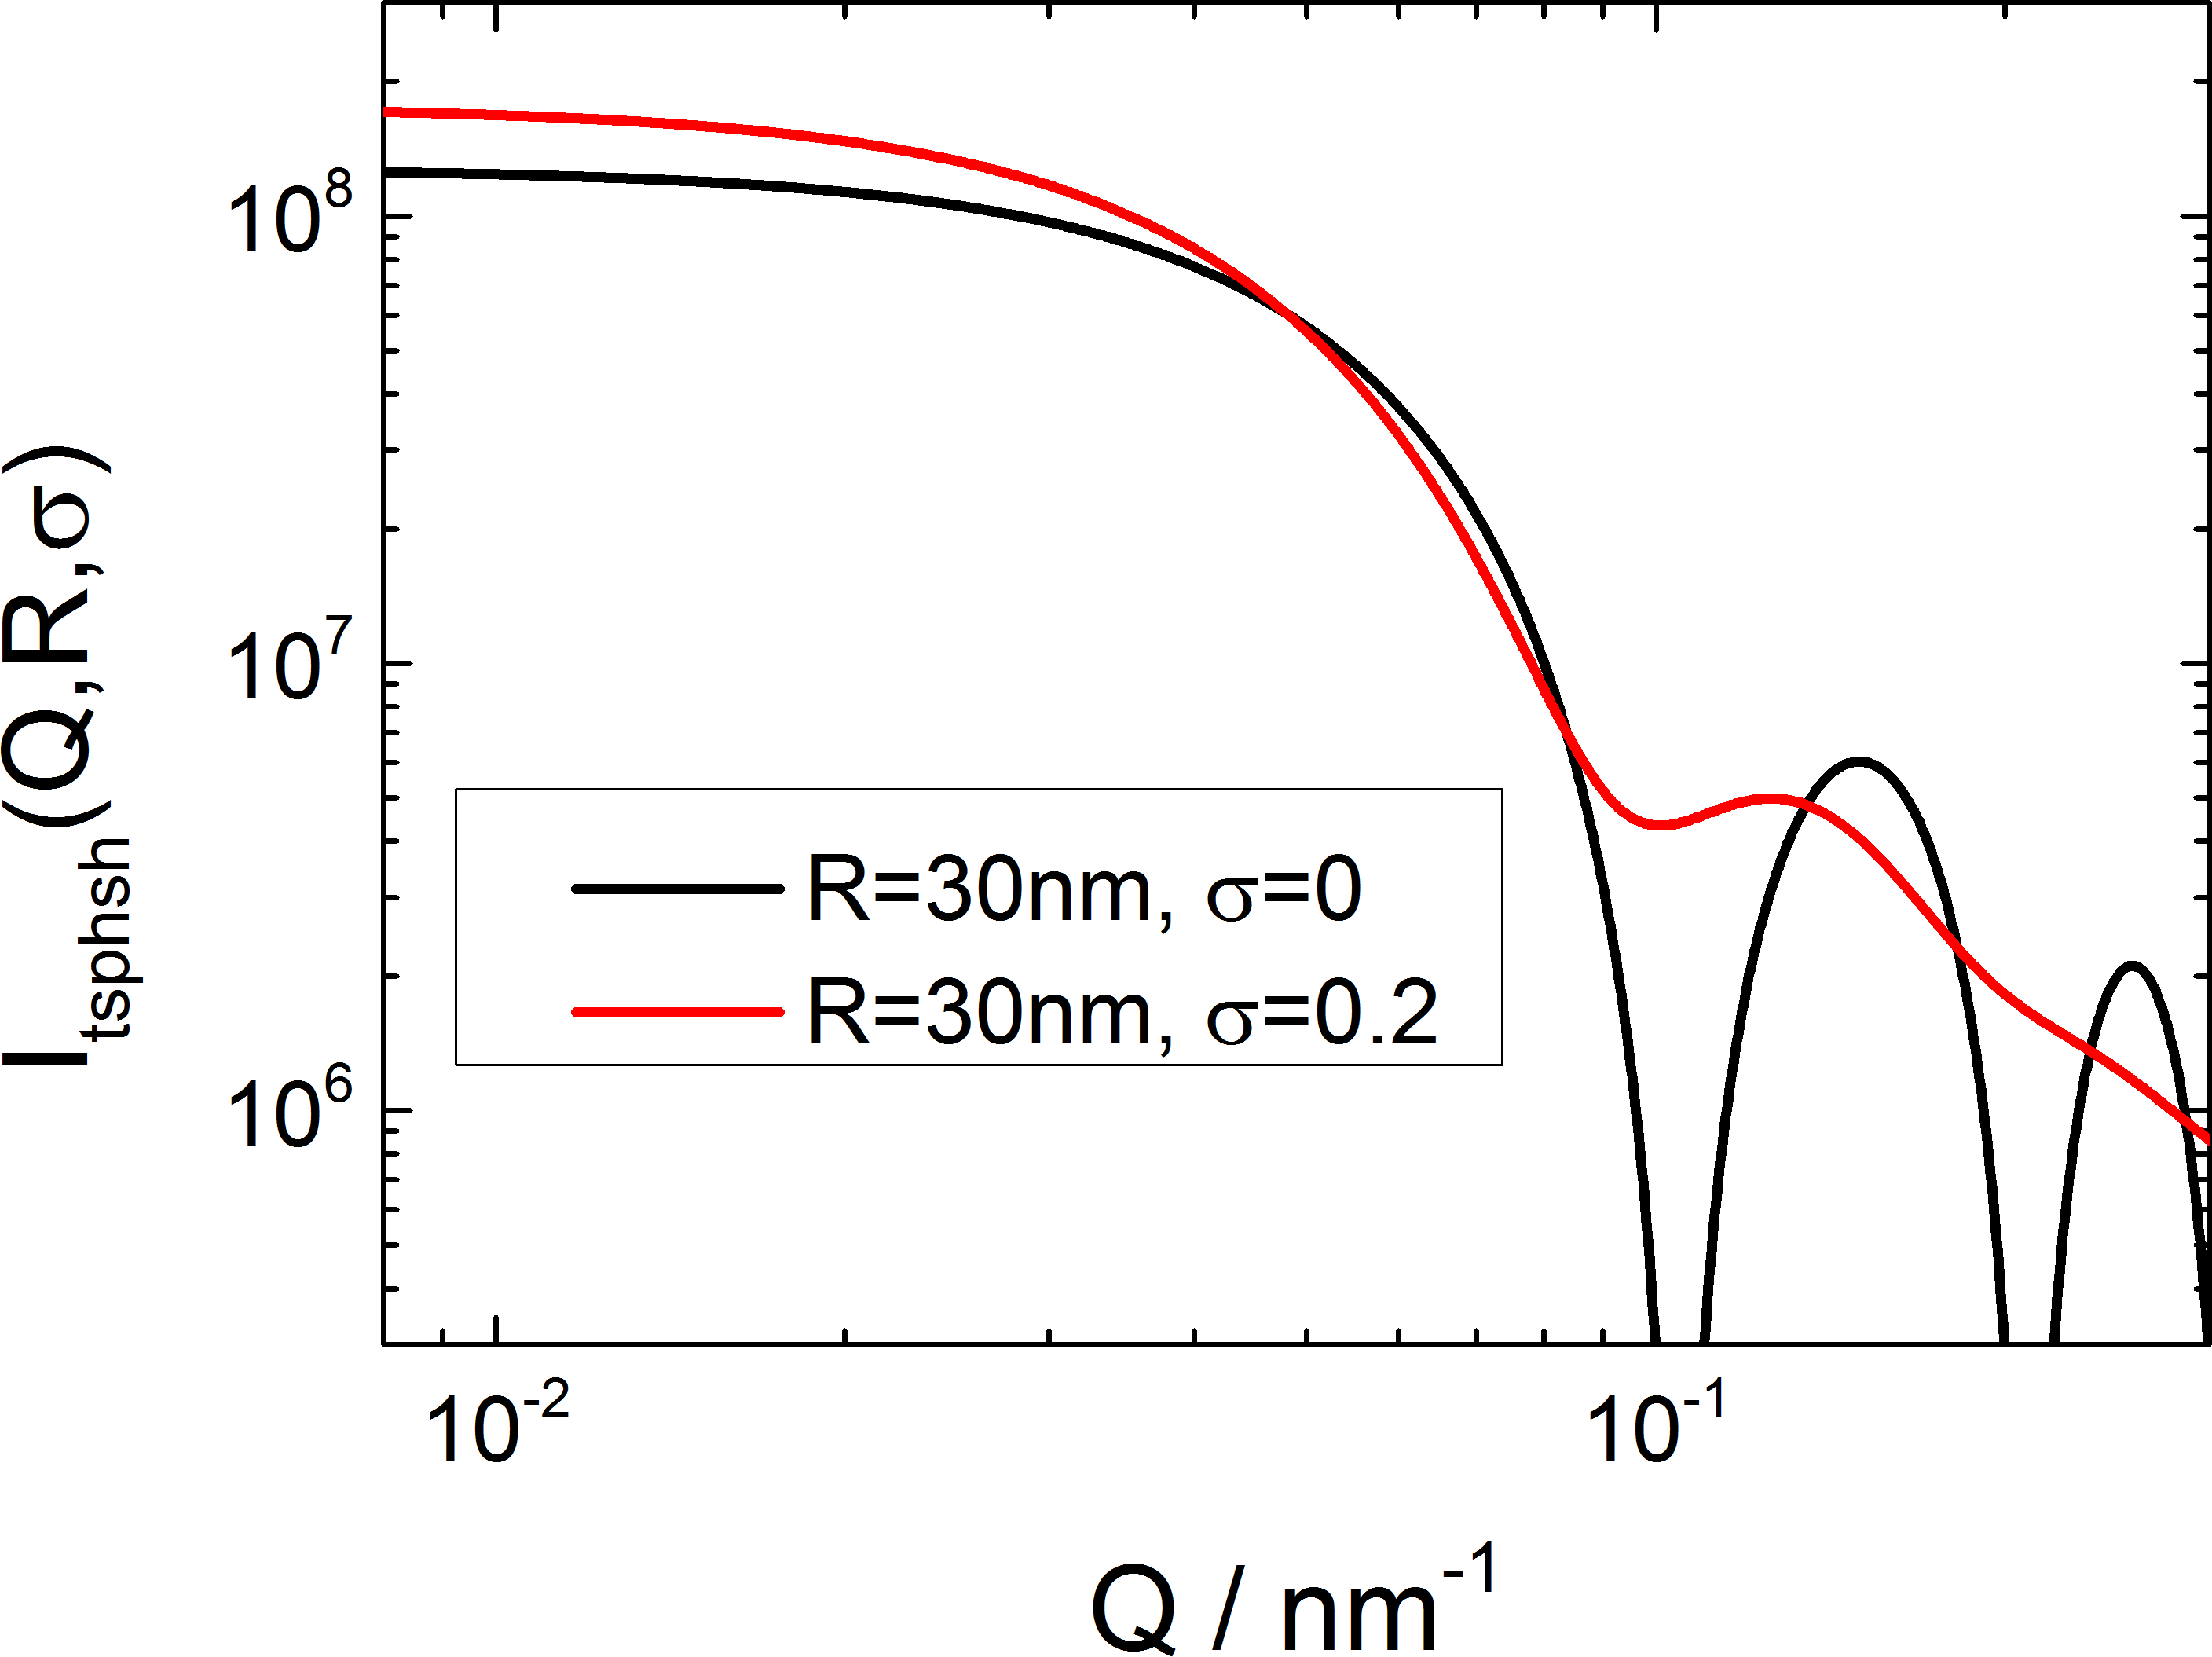
\includegraphics[width=0.8\textwidth,height=0.55\textwidth]{../images/form_factor/anisotropic/PprimeThinSphShell.png}
\end{center}
\caption{Scattering curve for the structure factor "\texttt{P'(Q): Thin Spherical Shell}" in combination with a constant background of 1".}
\label{fig_IQ:PprimeThinSphShell}
\end{figure}


\clearpage
\subsubsection{P'(Q): thin ellipsoidal shell} ~\\
\label{plugin:Pprime4ellShell}

\begin{figure}[htb]
\begin{center}
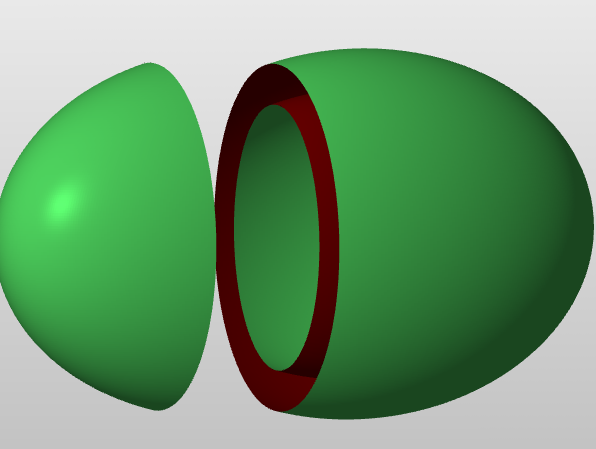
\includegraphics[width=0.596\textwidth,height=0.449\textwidth]{../images/form_factor/anisotropic/Ellipsoid_hollow.png}
\end{center}
\caption{Sketch of a thin ellipsoidal shell with a radius $R$ and eccentricity $\epsilon$. The thickness of the shell is assumed to be much smaller than the two radii of the elliptical shell.}
\label{fig:ThinEllipsoidalShell}
\end{figure}

\noindent
\textbf{Input parameters for \texttt{P'(Q): Thin Ellipsoidal Shell}:}
\begin{description}
    \item[\texttt{R}] most probable radius $R$
    \item[\texttt{epsilon}] eccentricity $\epsilon$
    \item[\texttt{sima\_R}] width $\sigma_R$ of radius distribution (LogNorm)
\end{description}

\noindent
\textbf{Note}
\begin{itemize}
  \item This structure factor is supposed to be combined with a form factor of local planar objects which are implemented as form factor plugins
under "\texttt{[by plugin|anisotropic obj.|Pcs(Q): local planar obj.]}".
\item The structure factor already has a log-normal width distribution for one parameter included.
\end{itemize}

\begin{figure}[htb]
\begin{center}
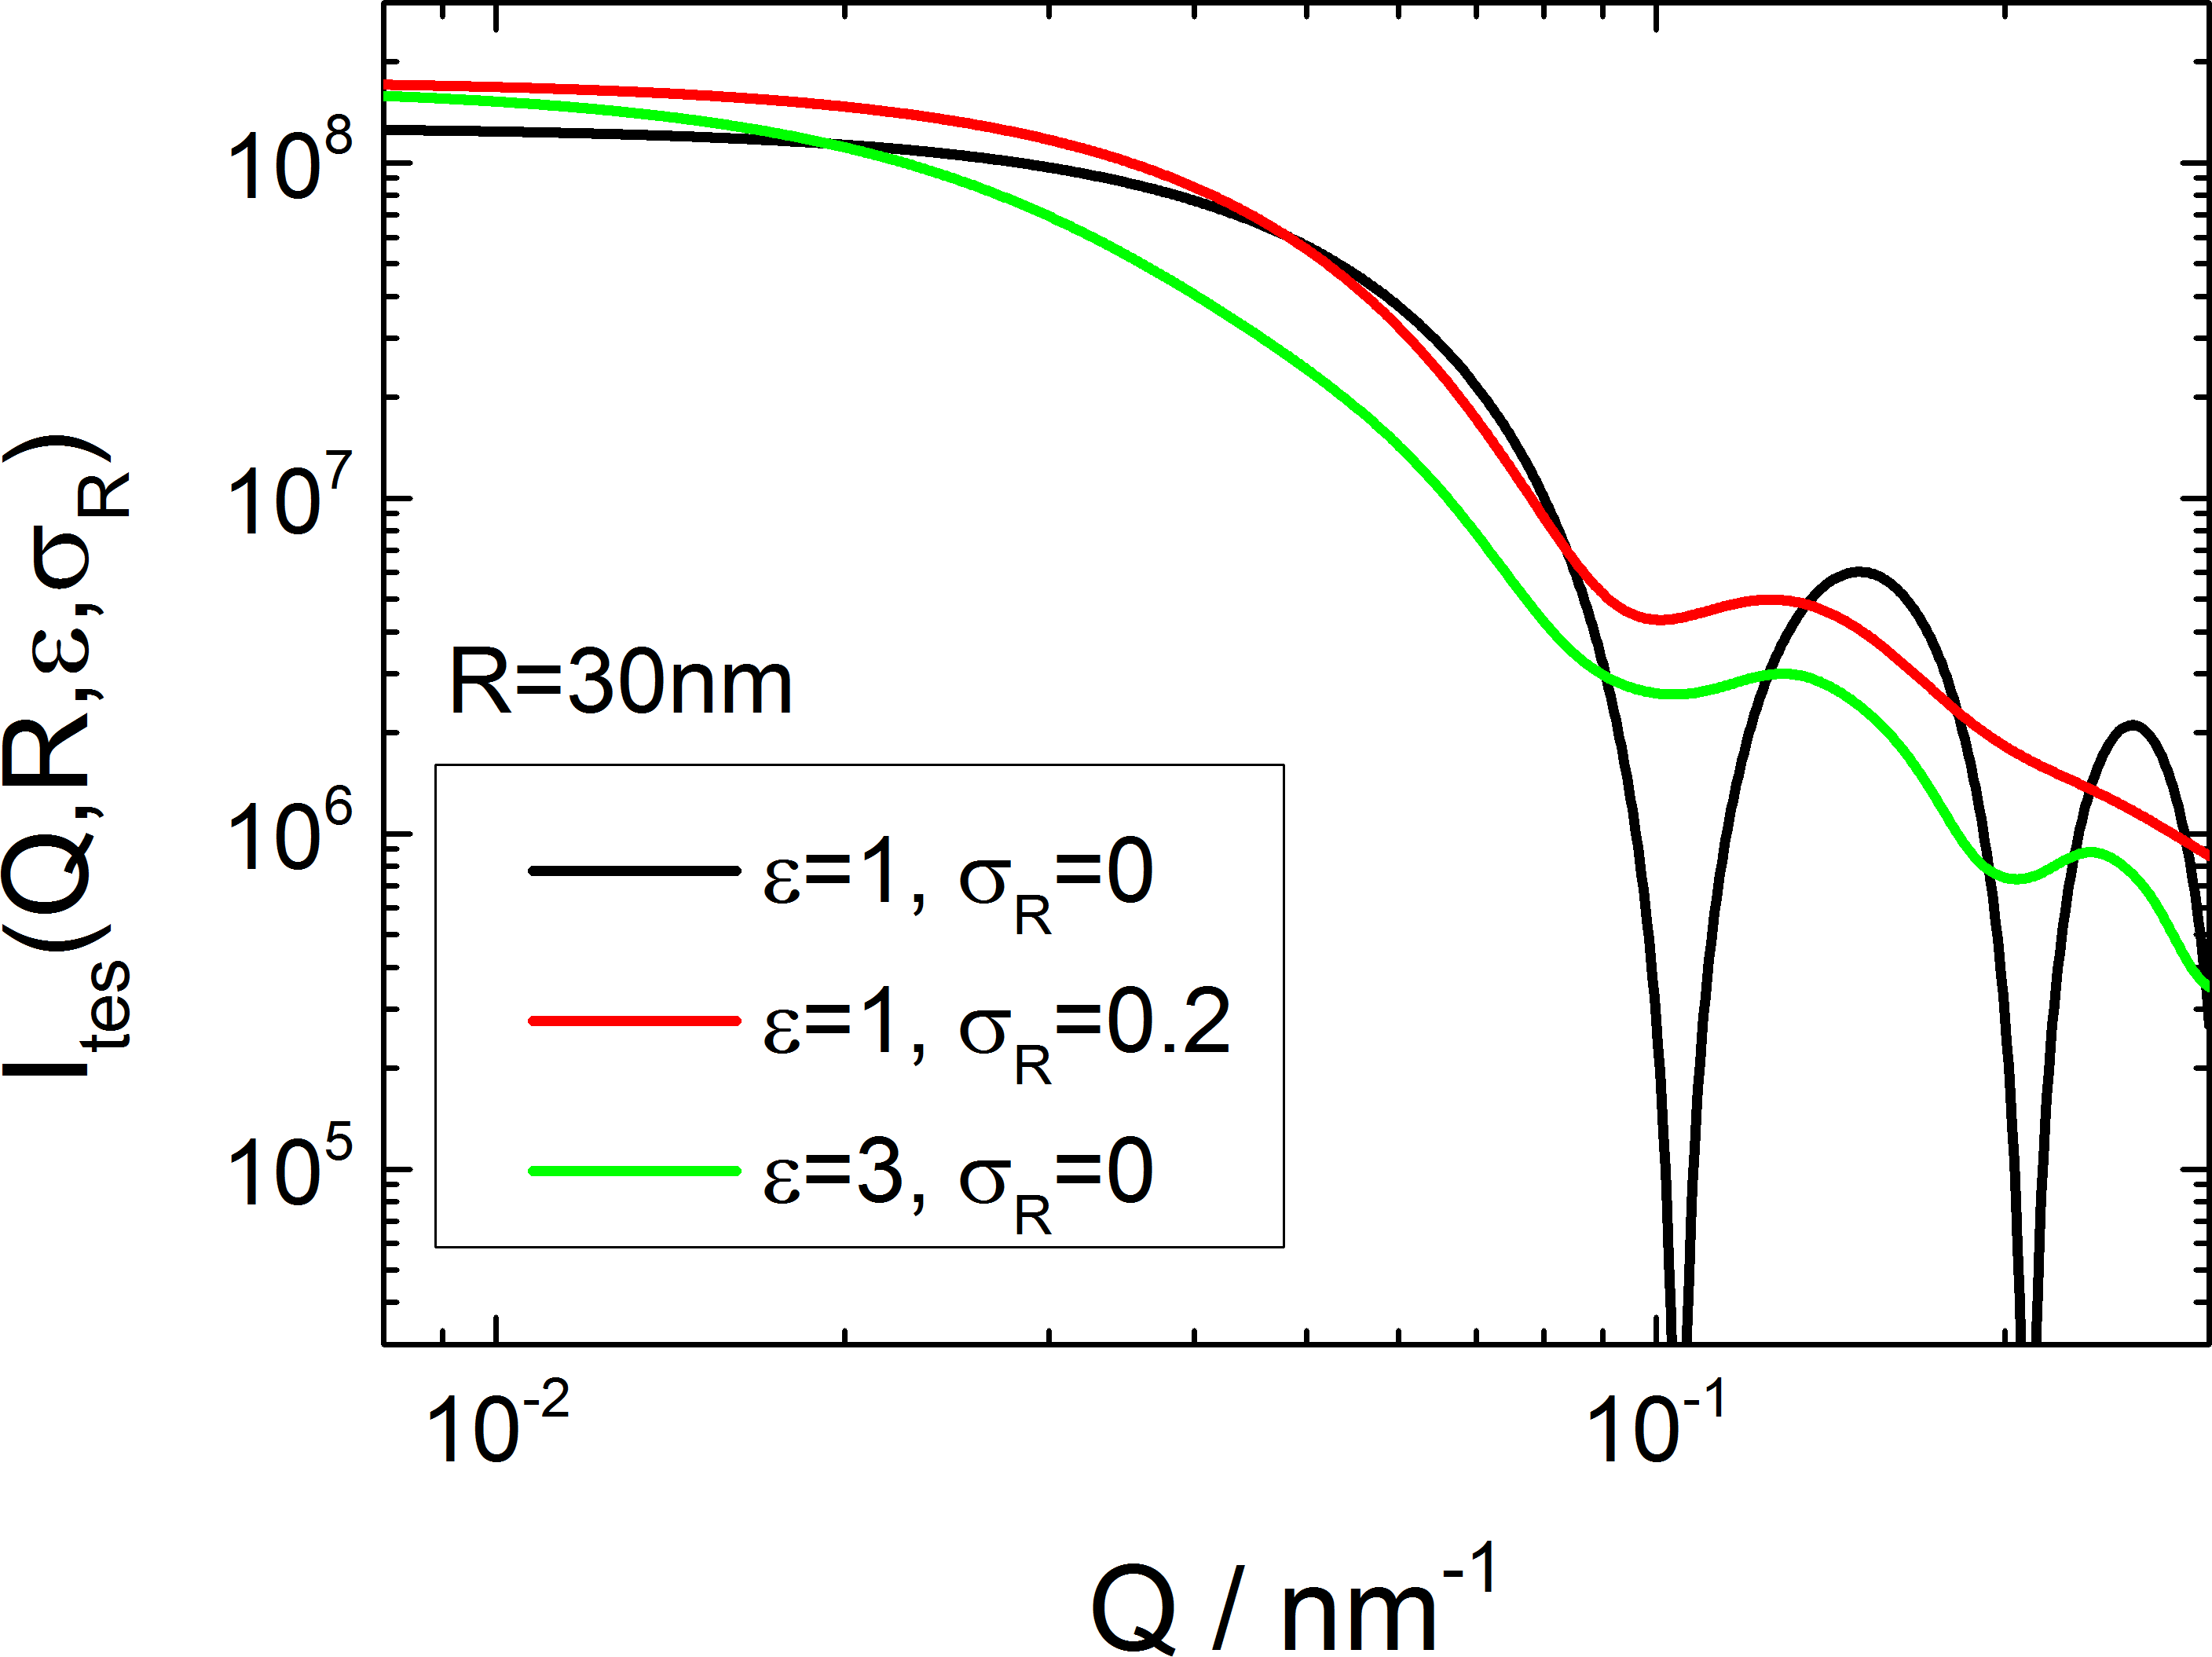
\includegraphics[width=0.8\textwidth,height=0.55\textwidth]{../images/form_factor/anisotropic/PprimeThinEllShell.png}
\end{center}
\caption{Scattering curve for the structure factor "\texttt{P'(Q): Thin Ellipsoidal Shell}" in combination with a constant background of 1".}
\label{fig_IQ:PprimeThinEllShell}
\end{figure}

\clearpage
\subsubsection{P'(Q): thin hollow cylinder} ~\\
\label{plugin:Pprime4hollowcylinder}

\begin{figure}[htb]
\begin{center}
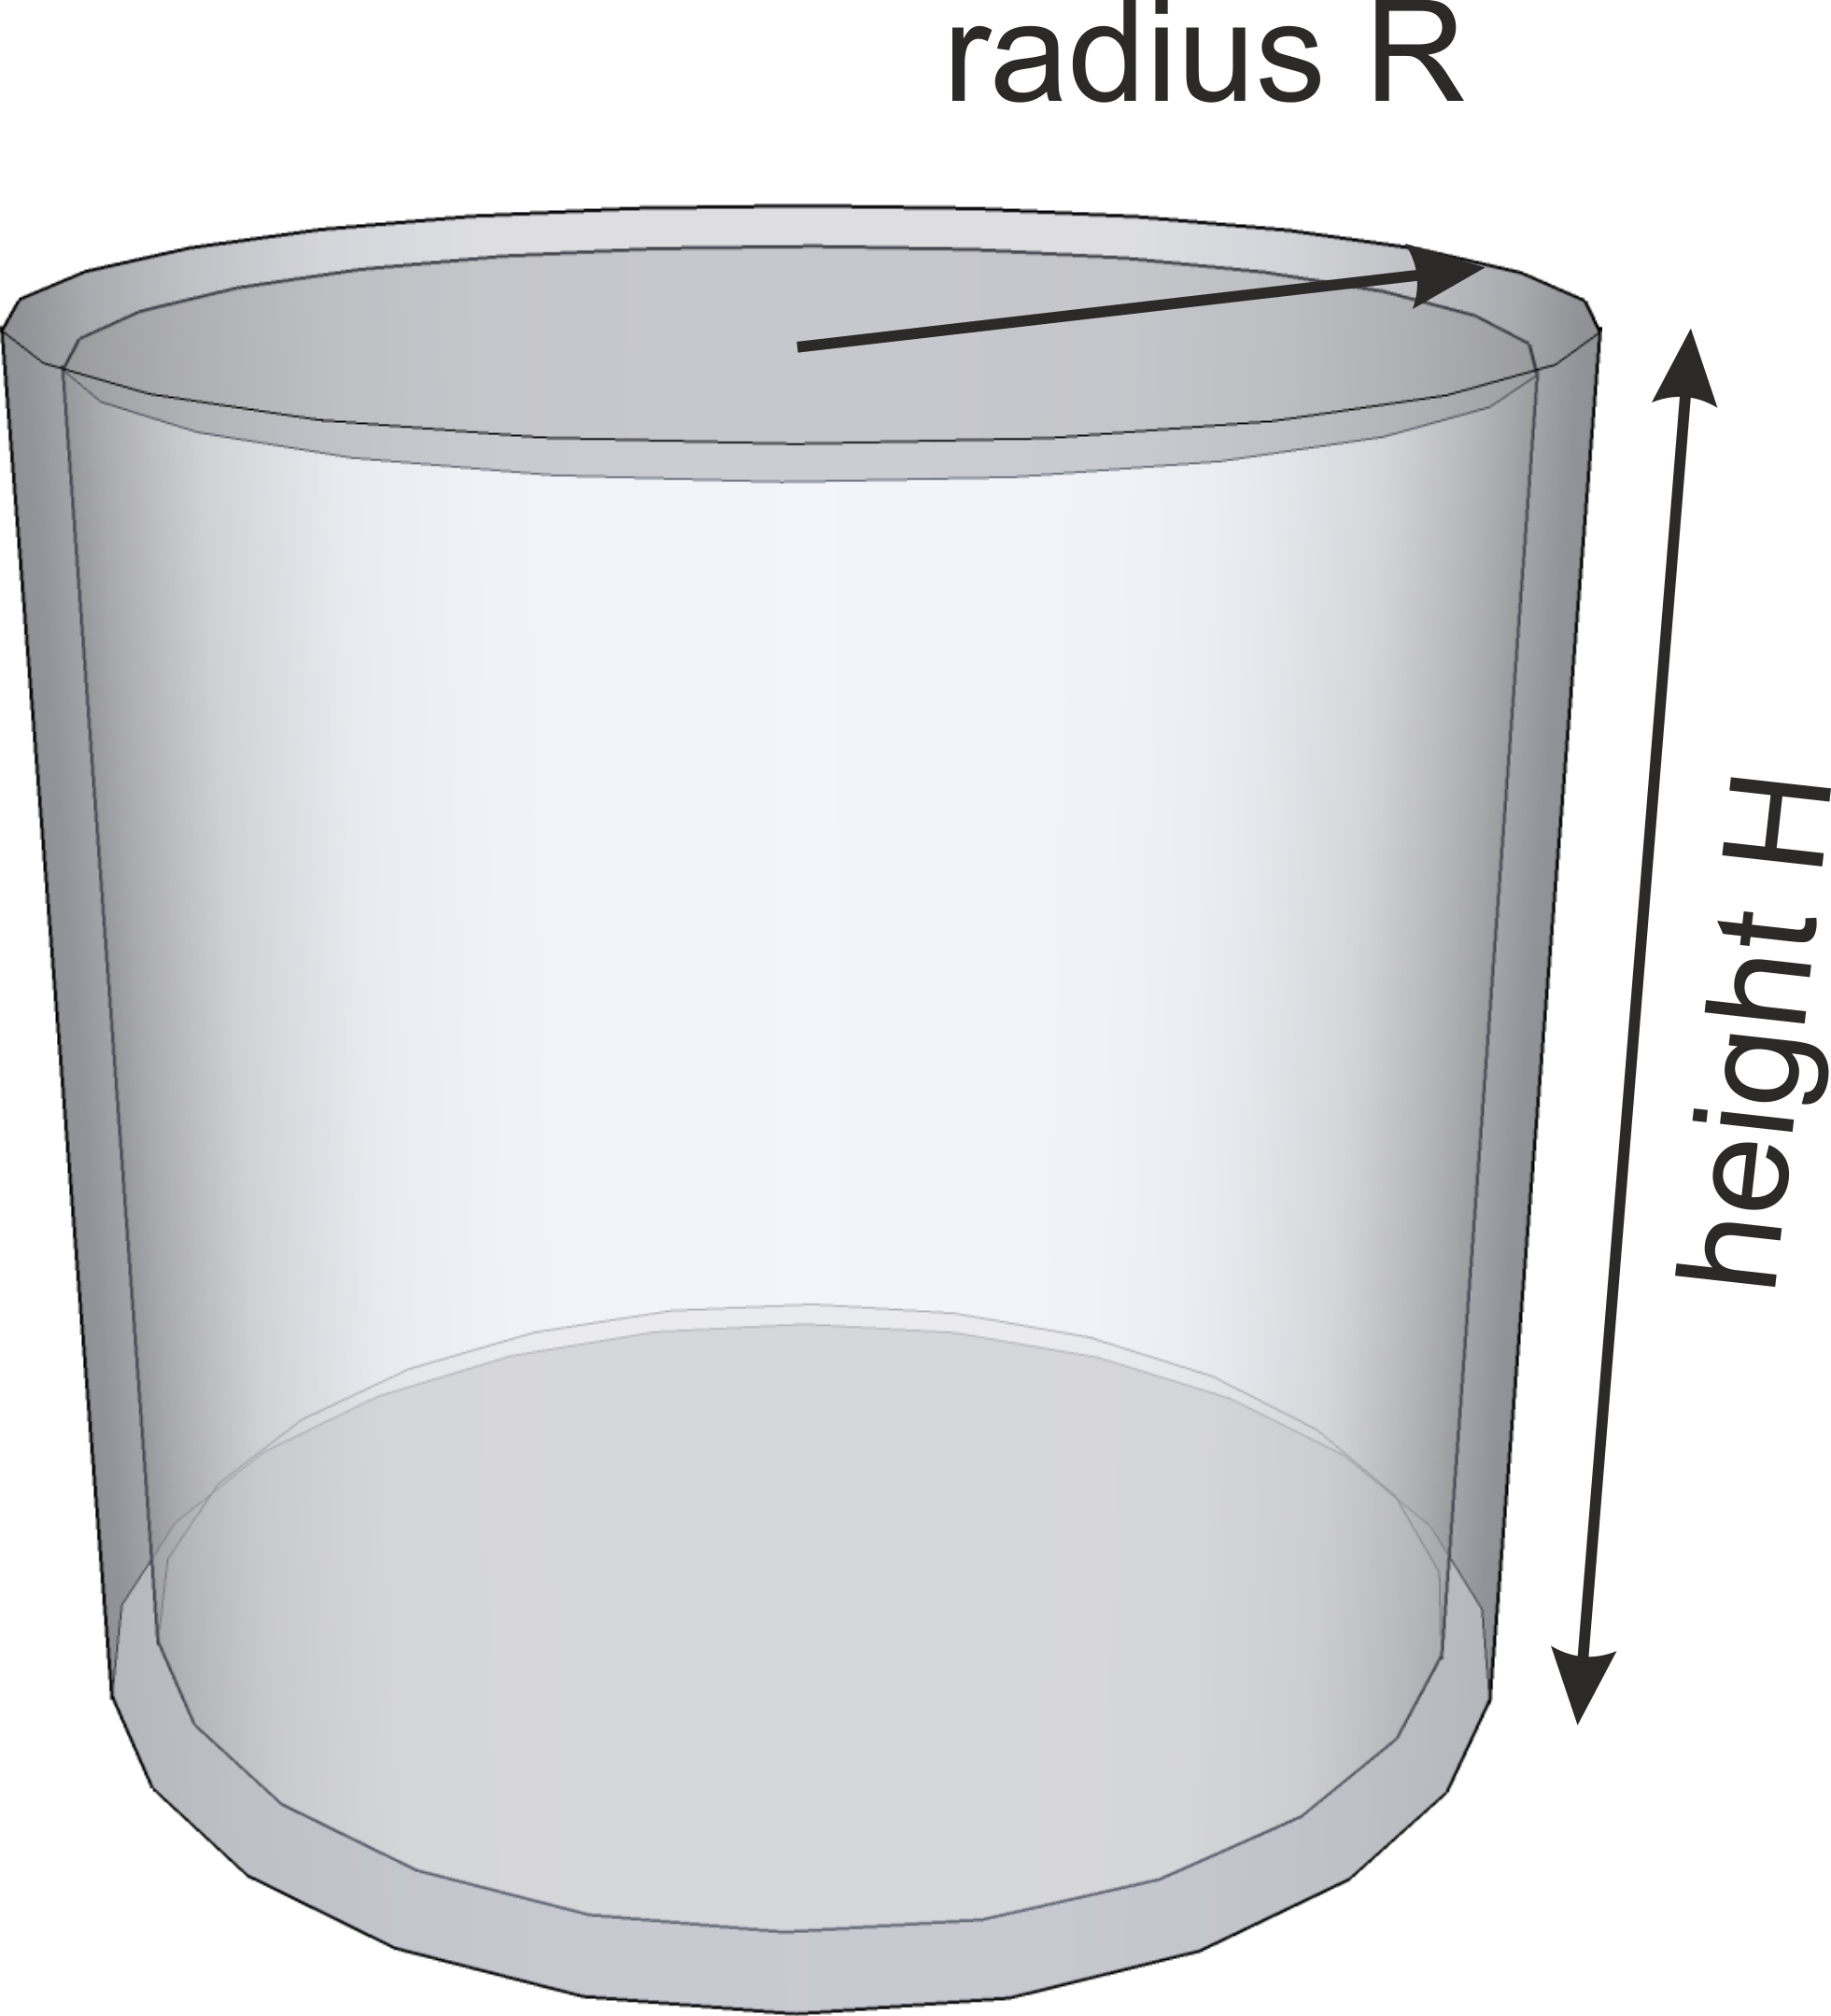
\includegraphics[width=0.3922\textwidth,height=0.4318\textwidth]{../images/form_factor/anisotropic/ThinHollowCylinder.png}
\end{center}
\caption{Sketch of a thin hollow cylinder of height $H$ and radius $R$. The thickness of the wall is assumed to be much smaller than the outer dimensions of the cylinder.}
\label{fig:ThinHollowCylinder}
\end{figure}

\begin{align}
\begin{split}
\Xi(Q,R,H,\alpha) & = 2\pi R
\left[ R \frac{J_1\left(Q R \sin\alpha\right)}{Q R \sin\alpha} \right. \\
& \left. \quad \quad + H J_0\left( \frac{QH}{2} \cos\alpha\right)\frac{\sin\left(\frac{QH}{2} \cos\alpha\right)}{\frac{QH}{2} \cos\alpha} \right]
\end{split} \\
P_\text{thc}(Q,R,H) &= \int_0^{\pi/2} \Xi^2(Q,R,H,\alpha) \sin\alpha \mathrm{d}\alpha \\
\begin{split}
I_{thc}(Q,R,H) &= \int_0^\infty \int_0^\infty
\mathrm{LogNorm}(r,1,\sigma_R,1,R,1) \\
& \qquad \qquad  \mathrm{LogNorm}(h,1,\sigma_H,1,H,1) P_\text{thc}(Q,r,h)
\, \mathrm{d}h \, \mathrm{d}r
\end{split}
\end{align}

\noindent
\textbf{Input parameters for \texttt{P'(Q): Thin Hollow Cylinder}:}
\begin{description}
    \item[\texttt{R}] most probable cylinder radius $R$
    \item[\texttt{H}] most probable cylinder height $H$
    \item[\texttt{sima\_R}] width $\sigma_R$ of radius distribution (LogNorm)
    \item[\texttt{sima\_H}] width $\sigma_H$ of height distribution (LogNorm)
\end{description}

\noindent
\textbf{Note}
\begin{itemize}
  \item This structure factor is supposed to be combined with a form factor of local planar objects which are implemented as form factor plugins
under "\texttt{[by plugin|anisotropic obj.|Pcs(Q): local planar obj.]}".
\item The structure factor already has a log-normal width distribution for one parameter included.
\end{itemize}

\begin{figure}[htb]
\begin{center}
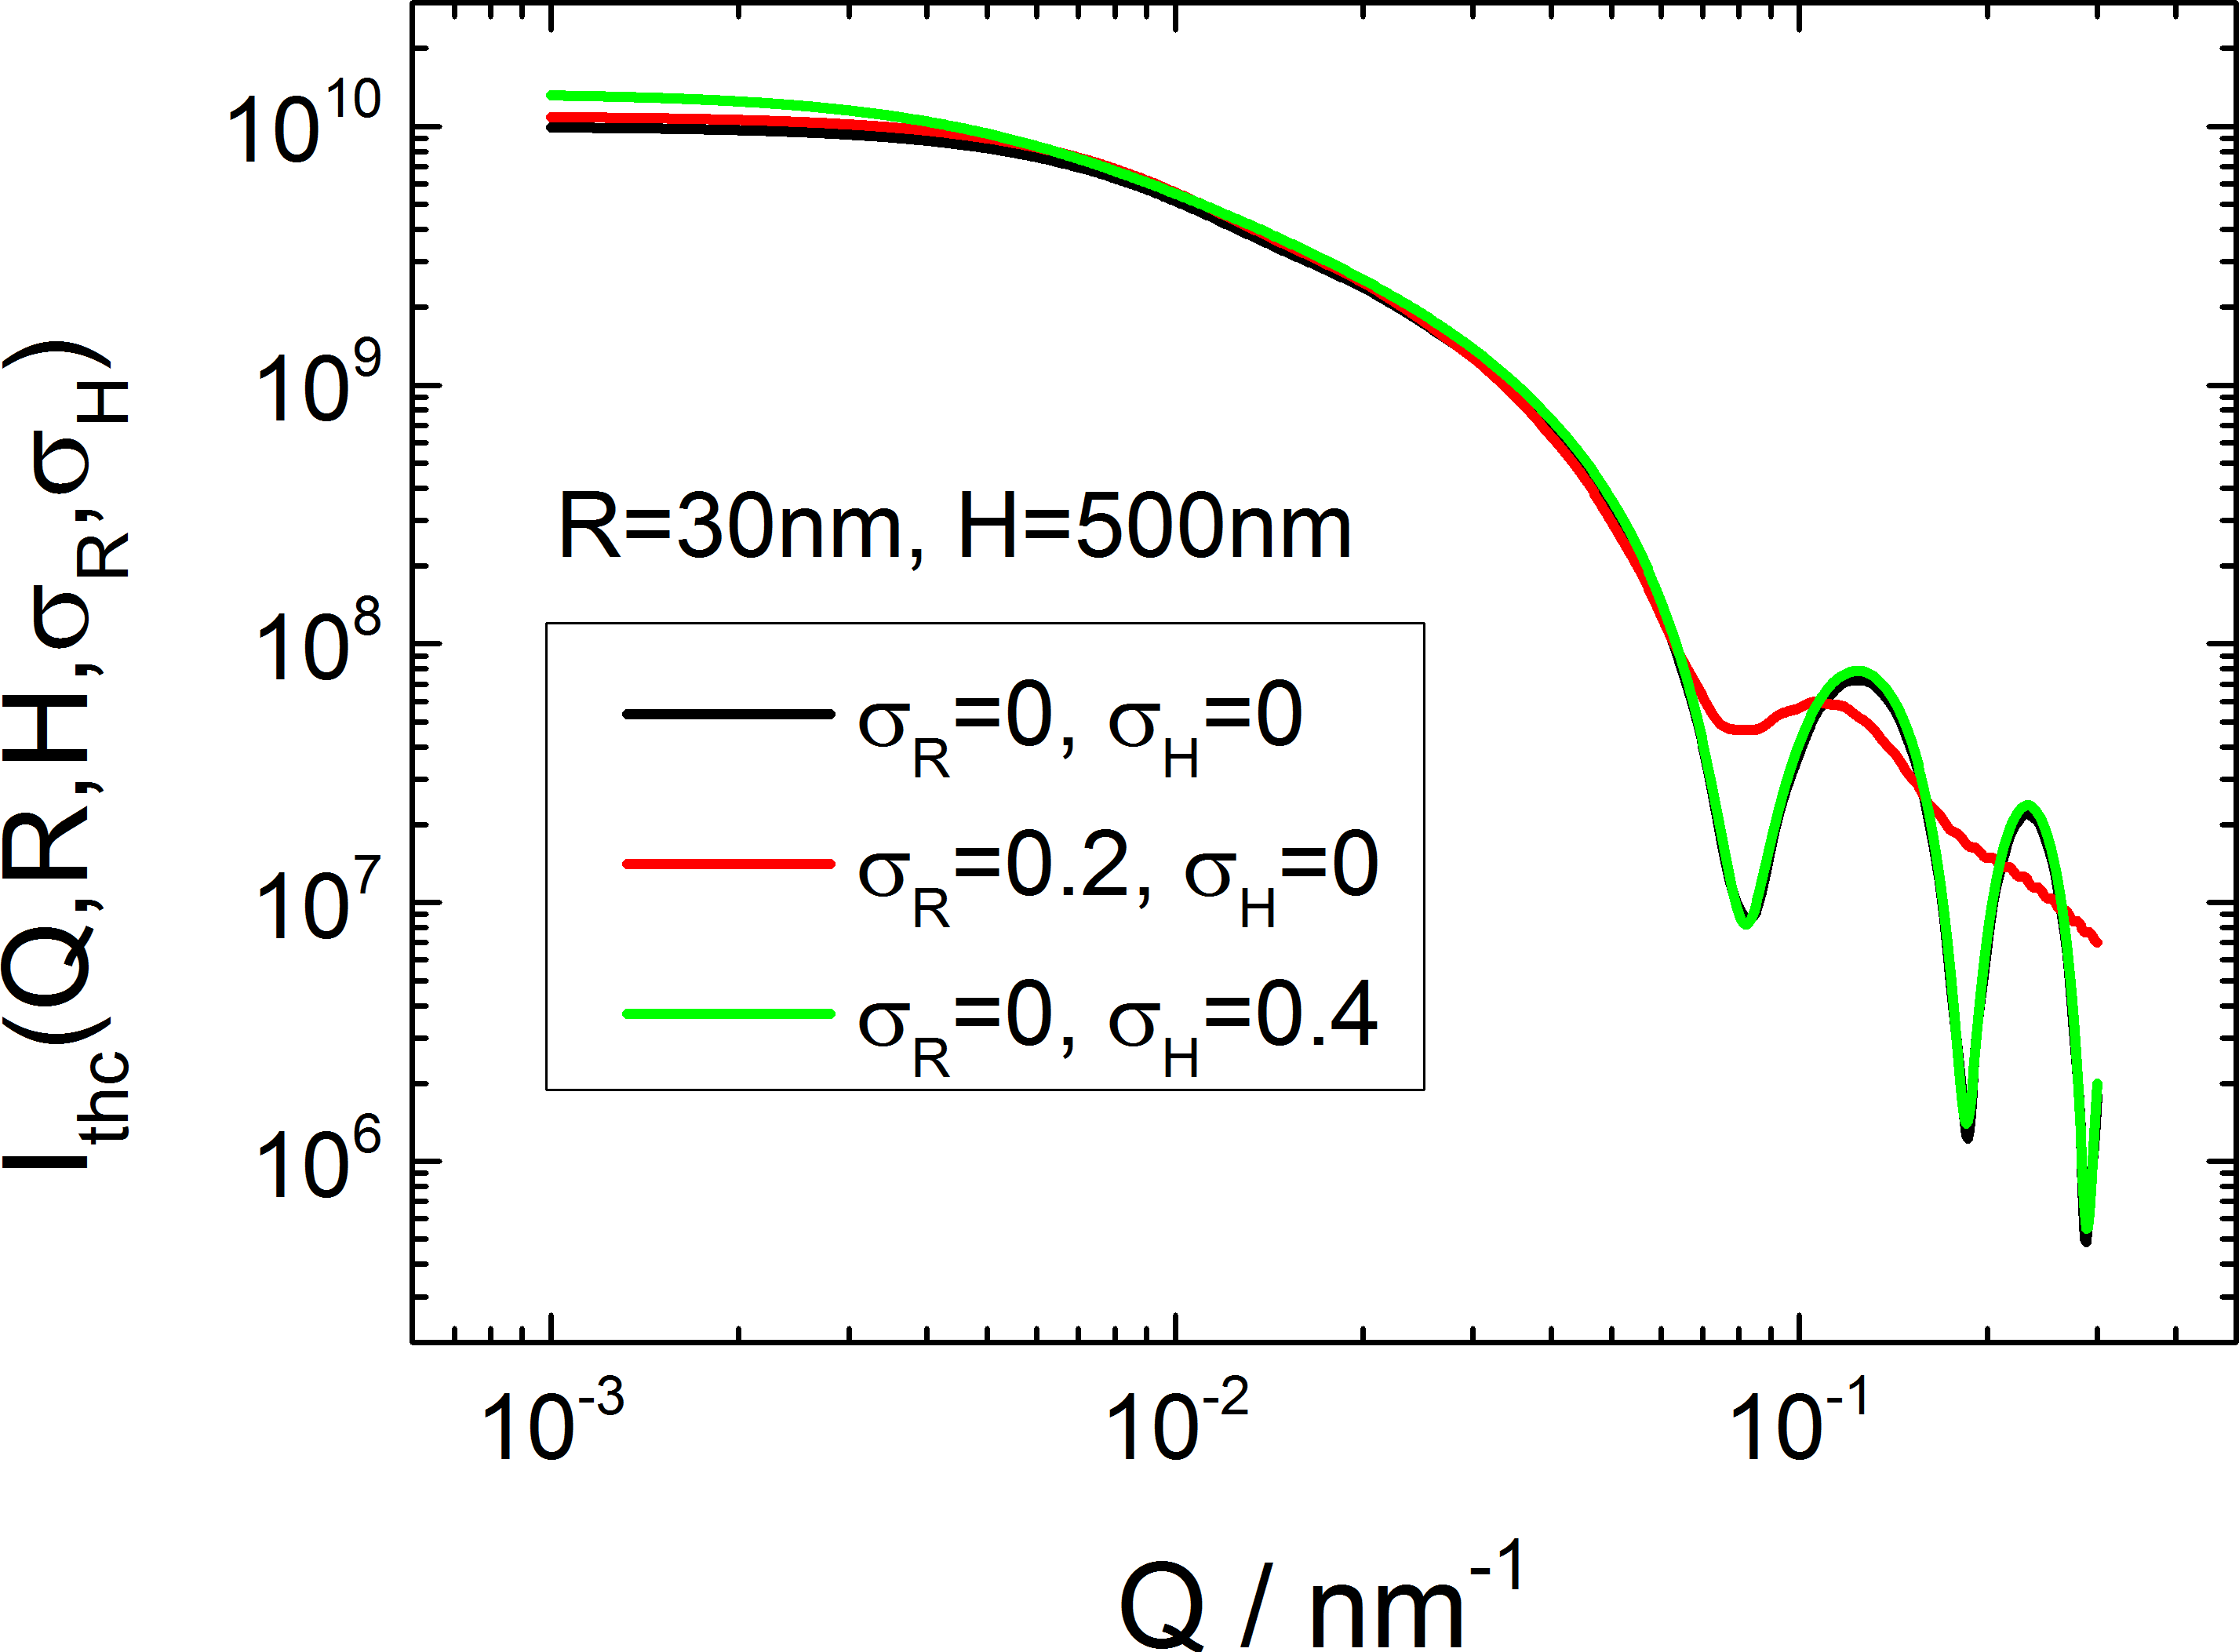
\includegraphics[width=0.8\textwidth,height=0.55\textwidth]{../images/form_factor/anisotropic/PprimeThinHollowCylinder.png}
\end{center}
\caption{Scattering curve for the structure factor "\texttt{P'(Q): Thin Hollow Cylinder}" in combination with a constant background of 1".}
\label{fig_IQ:PprimeThinHollowCylinder}
\end{figure}


\clearpage
\subsection{P'(Q) for local cylindrical obj.} ~\\
\label{plugin:Pprime4cylindrical}


\clearpage
\subsubsection{P'(Q): rods} ~\\
\label{plugin:Pprime4rods}

\begin{figure}[htb]
\begin{center}
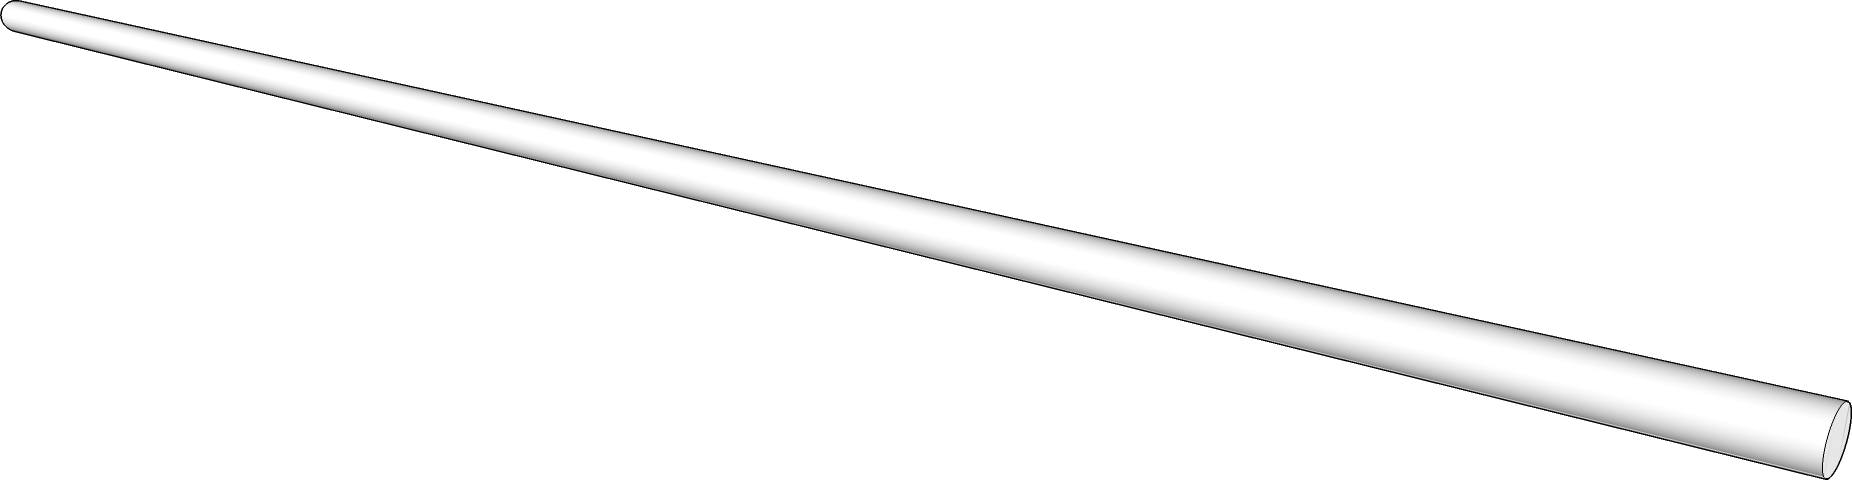
\includegraphics[width=0.926\textwidth,height=0.24\textwidth]{../images/form_factor/anisotropic/ThinRod.png}
\end{center}
\caption{Sketch of a thin Rod of Length $L$. The diameter of the rod is assumed to be much smaller than its length.}
\label{fig:ThinRod}
\end{figure}

\noindent
\textbf{Note}
\begin{itemize}
  \item This structure factor is supposed to be combined with a form factor with local cylindrical geometry which are implemented as form factor plugins
under "\texttt{[by plugin|anisotropic obj.|Pcs(Q): local cylindrical obj.]}".
\item The structure factor already has a log-normal width distribution for one parameter included.
\end{itemize}

\clearpage
\subsubsection{P'(Q): Kholodenko's worm} ~\\
\label{plugin:Pprime4kohlodenko}

\begin{figure}[htb]
\begin{center}
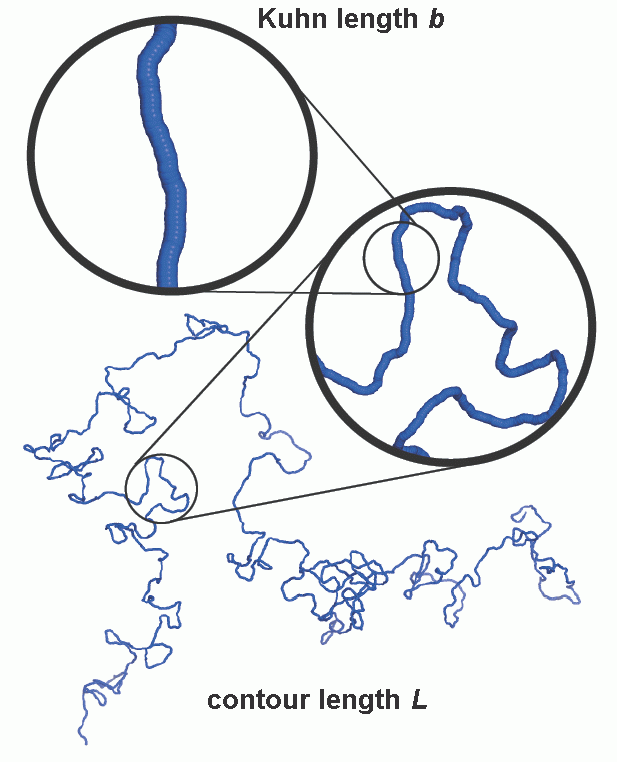
\includegraphics[width=0.617\textwidth,height=0.762\textwidth]{SemiflexiblePolymerTxt.png}
\end{center}
\caption{}
\label{fig:KholodenkoWorm}
\end{figure}

By using the analogy between Dirac’s fermions
and semi-flexible polymers
Kholodenko \cite{kholodenko93} could give a simple expression for the
scattering behaviour of wormlike structures. The form factor $P_0(Q)$ resulting
from Kholodenko’s approach is designed to reproduce
correctly the rigid-rod limit and the random-coil limit.
Defining $x = 3L/l_b$ ($L$: contour length, $l_b$: Kuhn length), it is given by
\begin{align}
P_0(Q,L,l) &= \frac{2}{x} \left[I_{(1)} -\frac{1}{x}I_{(2)}\right]
\label{eq:KholodenkoPprime}
\end{align}
where
\begin{align}
I_{(n)}(x) &= \int_0^x  f(z) \, z^{n-1} \, dz
\end{align}
together with
\begin{align}
f(z)) &=
\begin{cases} \displaystyle
\frac{1}{E}\frac{\sinh(Ez)}{\sinh(z)} & \text{for} \quad \displaystyle Q \leq \frac{3}{l}\\ \\
\displaystyle
\frac{1}{F}\frac{\sin(Fz)}{\sinh(z)} & \text{for} \quad \displaystyle Q > \frac{3}{l}
\end{cases}
\end{align}
and
\begin{align}
E = \sqrt{1-\left(\frac{lQ}{3}\right)^2} \quad \text{and} \quad F = \sqrt{\left(\frac{lQ}{3}\right)^2-1}
\end{align}

\begin{align}
P(Q,L,l_b,R) = P_0(Q,L,l_b)\, P_{cs}(Q,R)
\end{align}

\vspace{5mm}

\hspace{1pt}\\
\underline{Input Parameters for model \texttt{P'(Q) Kholodenko Worm}:}\\
\begin{description}
\item[\texttt{lb}] Kuhn length\footnote{The Kuhn length $l_b$ is related to the length $a$ of
    locally stiff segment simply via $l_b=2a$} $l$ of semi-flexible worm-like structure
\item[\texttt{L}] contour length $L$ of semi-flexible worm-like structure
\end{description}

\noindent
\textbf{Note}
\begin{itemize}
  \item This structure factor is supposed to be combined with a form factor with local cylindrical geometry which are implemented as form factor plugins
under "\texttt{[by plugin|anisotropic obj.|Pcs(Q): local cylindrical obj.]}".
\item The structure factor already has a log-normal width distribution for one parameter included.
\item The equivalent solution of J.S. Pedersen \cite{Pedersen96Macrom} would be the expressions of wormlike structures without excluded volume effects.
\end{itemize}

\clearpage
\subsubsection{P'(Q): wormlike PS1} ~\\
\label{plugin:Pprime4wormPS1}

For worm-like micelles J.S. Pedersen \cite{Pedersen96Macrom} has developed three models
for worm-like micelles, from which one is basing on a method developed by Yoshizaki et al.\ \cite{Yoshizaki1980}.

~\\
\paragraph*{\textbf{Without Excluded Volume Effects.}}~\\

This first of the three solutions given by J.S. Pedersen \cite{Pedersen96Macrom} for
worm-like micelles starts from the expression for the scattering function as follows:
\begin{align}
\label{eq:SWC}
\begin{split}
S_\text{WC}(Q,L,l_B) &= L^2 \left[  \left(1-\chi(Q,L,l_B)\right)
            S_\text{chain}(Q,L,l_B) \right. \\
&  \left. \qquad  \qquad  +\chi(Q,L,l_B) S_\text{rod}(Q,L)    \right] \Gamma(Q,L,l_B)
\end{split}
\end{align}
where $S_\text{chain}(Q,L,l_B)$ is the scattering function of a flexible
chain without excluded volume effects and $S_\text{rod}(Q,L)$ is
the scattering function of a rod. Furthermore, $\chi(Q,L,l_b)$
is a crossover function, and the function $\Gamma(q,L,b)$ corrects
the crossover region.
The function $S_\text{chain}(Q,L,l_B)$ is given by the Debye function:
\begin{align}
\label{eq:SDebye}
S_\text{chain}(Q,L,l_B) &= S_\text{Debye}(Q,L,l_B) = 2\left[\exp(-u)+u-1\right]/u^2
\end{align}
with $u=\left\langle R_g^2\right\rangle_0 Q^2 $, where $\left\langle R_g^2\right\rangle_0$
is the ensemble average of the square of the radius of gyration and given by
\begin{align}
\left\langle R_g^2\right\rangle_0 &= \frac{Ll_B}{6}\left[1
        -\frac{3}{2n_B}
        +\frac{3}{2n_B^2}
        -\frac{3}{4n_B^3}
        \left[1-\exp(-2n_B)\right]\right]
\end{align}
where $n_B=L/l_B$ b is the number of statistical segments of the chain.
The function $S\text{rod}(Q,L)$ in \ref{eq:SWC} is the scattering function
of an infinitely thin rod
\begin{align}
S_\text{rod}(Q,L) &= 2 \text{Si}(Q,L)/(QL)-4\sin^2(QL/2)/(QL)^2
\end{align}
where
\begin{align}
\text{Si}(Q,L) &= \int_0^x t^{-1} \sin t \; \mathrm{d}t
\end{align}
Furthermore we have
\begin{align}
\chi(Q,L,l_B) &= \exp\left(-\xi^{-5}\right)
\end{align}
The parameter $\xi$ is given by
\begin{align}
\xi &= Q\frac{\pi}{2L} \left\langle R_g^2\right\rangle_0
\end{align}
The function $\Gamma(Q,L,l_B)$ is given by
\begin{align}
\Gamma(Q,L,l_B) &= 1+(1-\chi)\sum_{i=2}^5A_i\xi^i + \chi\sum_{i=0}^2B_i\xi^{-i}
\end{align}
where
\begin{align}
\begin{split}
A_i &= \sum_{j=0}^2a_1(i,j) \left(\frac{L}{l_B}\right)^{-j} \exp(-10 l_B/L) \\
& \qquad \qquad + \sum_{j=1}^2a_2(i,j) \left(\frac{L}{l_B}\right)^{j} \exp(-2 L/l_B)
\end{split}
\end{align}
and
\begin{align}
\begin{split}
B_i & = \sum_{j=0}^2b_1(i,j) \left(\frac{L}{l_B}\right)^{-j} \\
    & \qquad \qquad + \sum_{j=1}^2b_2(i,j) \left(\frac{L}{l_B}\right)^{j} \exp(-2 L/l_B)
\end{split}
\end{align}
The values of $a_1(i,j), a_2(i,j), b_1(i,j)$, and $b_2(i,j)$ are listed in table \ref{table:numValWMPS1noexv}
\begin{table}
  \caption{Values for the parameters in the numerical expressions for the scattering function for worm-like chains \textbf{without} excluded volume effects \cite{Pedersen96Macrom}}
  \label{table:numValWMPS1noexv}
  \centering
  \begin{tabular}{l c|l c|l c|l c}
     \hline
     % after \\: \hline or \cline{col1-col2} \cline{col3-col4} ...
               &          &           &          & $b_1(0,0)$ & -0.0162  &            &          \\
               &          &           &          & $b_1(1,0)$ &  0.09046 &            &          \\
     $a1(2,0)$ &  0.3054  &           &          & $b_1(2,0)$ &  0.1213  &            &          \\
     $a1(3,0)$ &  0.05777 &           &          &            &          &            &          \\
     $a1(4,0)$ & -0.00604 &           &          &            &          &            &          \\
     $a1(5,0)$ & -0.03902 &           &          &            &          &            &          \\
               &          &           &          & $b_1(0,1)$ & -0.3565  & $b_2(0,1)$ & -0.3946  \\
               &          &           &          & $b_1(1,1)$ &  0.1909  & $b_2(1,1)$ & -0.2231  \\
     $a1(2,1)$ &  0.2316  & $a2(2,1)$ & -0.4963  & $b_1(2,1)$ &  0.15634 & $b_2(2,1)$ & -0.2546  \\
     $a1(3,1)$ &  0.26531 & $a2(3,1)$ &  0.03688 &            &          &            &          \\
     $a1(4,1)$ &  0.3706  & $a2(4,1)$ &  0.30570 &            &          &            &          \\
     $a1(5,1)$ & -1.0081  & $a2(5,1)$ &  0.39013 &            &          &            &          \\
               &          &           &          & $b_1(0,2)$ & -0.3078	 & $b_2(0,2)$ &  1.1361  \\
               &          &           &          & $b_1(1,2)$ &  0.05176 & $b_2(1,2)$ & -0.01615 \\
     $a1(2,2)$ & -22.779  & $a2(2,2)$ & -0.4678  & $b_1(2,2)$ &  0.01568 & $b_2(2,2)$ & -0.07606 \\
     $a1(3,2)$ &  23.2457 & $a2(3,2)$ &  0.3365  &            &          &            &          \\
     $a1(4,2)$ &  8.1092  & $a2(4,2)$ &  0.4290  &            &          &            &          \\
     $a1(5,2)$ & -3.3603  & $a1(5,2)$ &  0.3737  &            &          &            &          \\
     \hline
   \end{tabular}
\end{table}

~\\
\paragraph*{\textbf{With Excluded Volume Effects.}}~\\

To include excluded volume effects in eq.\ \ref{eq:SWC} the function for a flexible chain $S_\text{chain}(Q,L,l_B)$ needs to be replaced by one with excluded volume effects included
\begin{align}
\label{eq:exvSWC}
\begin{split}
S_\text{WC}(Q,L,l_B) &= L^2 \left[  \left(1-\chi(Q,L,l_B)\right)
            S_\text{exv}(Q,L,l_B) \right. \\
&  \left. \qquad  \qquad  +\chi(Q,L,l_B) S_\text{rod}(Q,L)    \right] \Gamma(Q,L,l_B)
\end{split}
\end{align}
The scattering of a chain with excluded volume effects is given by
\begin{multline}
S_\text{exv}(Q,L,l_B) = w(Q,R_g) S_\text{Debye}(Q,L,l_B) + \\
 \left[1-w(q R_g)\right[\left[C_1\left(QR_g\right)^{-1/\nu}
                                           + C_2\left(QR_g\right)^{-2/\nu}
                                           + C_3\left(QR_g\right)^{-3/\nu}\right]
\end{multline}
where $S_\text{Debye}(Q,L,l_B)$ is given by eq.\ \ref{eq:SDebye} and
\begin{align}
R_g^2&=\alpha(L/l_B)^2 \langle R_g^2\rangle^2
\label{eq:RgexvWC}
\end{align}
with $\alpha(L/l_B)$ being an expansion factor following the expression:
\begin{align}
\alpha(x)^2 &= \left[ 1+(x/3.12)^2+(x/8.67)^3 \right]^{\epsilon/3}
\end{align}
and $\epsilon=0.170$. The function $w(x)$ is another empirical cross-over function chosen as:
\begin{align}
w(x) &= \left[ 1+\tanh\left(\frac{x-C_4}{C_5}\right)/C_5 \right]/2
\end{align}
The parameters $C_i$ have been given in \cite{Pedersen96Macrom} as
$C_1=1.220$, $C_2=0.4288$, $C_3=-1.651$, $C_4=1.523$, and $C_5=0.1477$.

Furthermore the parameter $\xi$ in the cross-over function $\chi(Q,L,l_B)$ needs to be chosen as
\begin{align}
\xi&=Ql_B\left(\frac{\pi l_B}{1.103 L}\right)^{3/2}\left[\frac{R_g^2}{l_B^2}\right]^{1.282}
\end{align}
with $R_g^2$ defined in eq.\ \ref{eq:RgexvWC}. Last, but not least the values of $a_1(i,j), a_2(i,j), b_1(i,j)$, and $b_2(i,j)$ need to be taken from table \ref{table:numValWMPS1withexv}.
\begin{table}
  \caption{Values for the parameters in the numerical expressions for the scattering function for worm-like chains \textbf{with} excluded volume effects \cite{Pedersen96Macrom}}
  \label{table:numValWMPS1withexv}
  \centering
  \begin{tabular}{l c|l c|l c|l c}
     \hline
     % after \\: \hline or \cline{col1-col2} \cline{col3-col4} ...
               &          &           &          & $b_1(0,0)$ & -0.0699  &            &          \\
               &          &           &          & $b_1(1,0)$ & -0.0900  &            &          \\
     $a1(2,0)$ & -0.1222  &           &          & $b_1(2,0)$ &  0.2677  &            &          \\
     $a1(3,0)$ &  0.3051  &           &          &            &          &            &          \\
     $a1(4,0)$ & -0.0711  &           &          &            &          &            &          \\
     $a1(5,0)$ &  0.0584  &           &          &            &          &            &          \\
               &          &           &          & $b_1(0,1)$ &  0.1342  & $b_2(0,1)$ & -0.5171  \\
               &          &           &          & $b_1(1,1)$ &  0.0138  & $b_2(1,1)$ & -0.2028  \\
     $a1(2,1)$ &  1.761   & $a2(2,1)$ &  0.1212  & $b_1(2,1)$ &  0.1898  & $b_2(2,1)$ & -0.3112  \\
     $a1(3,1)$ &  2.252   & $a2(3,1)$ & -0.4169  &            &          &            &          \\
     $a1(4,1)$ & -1.291   & $a2(4,1)$ &  0.1988  &            &          &            &          \\
     $a1(5,1)$ &  0.6994  & $a2(5,1)$ &  0.3435  &            &          &            &          \\
               &          &           &          & $b_1(0,2)$ & -0.2020	 & $b_2(0,2)$ &  0.6950  \\
               &          &           &          & $b_1(1,2)$ & -0.0114  & $b_2(1,2)$ & -0.3238  \\
     $a1(2,2)$ & -26.04   & $a2(2,2)$ &  0.0170  & $b_1(2,2)$ &  0.0123  & $b_2(2,2)$ & -0.5403  \\
     $a1(3,2)$ &  20.00   & $a2(3,2)$ & -0.4731  &            &          &            &          \\
     $a1(4,2)$ &  4.382   & $a2(4,2)$ &  0.1869  &            &          &            &          \\
     $a1(5,2)$ &  1.594   & $a1(5,2)$ &  0.3350  &            &          &            &          \\
     \hline
   \end{tabular}
\end{table}


\noindent
\textbf{Note}
\begin{itemize}
  \item This structure factor is supposed to be combined with a form factor with local cylindrical geometry which are implemented as form factor plugins
under "\texttt{[by plugin|anisotropic obj.|Pcs(Q): local cylindrical obj.]}".
\item The structure factor already has a log-normal width distribution for one parameter included.
\end{itemize}

\clearpage
\subsubsection{P'(Q): wormlike PS2} ~\\
\label{plugin:Pprime4wormPS2}

\noindent
\textbf{Note}
\begin{itemize}
  \item This structure factor is supposed to be combined with a form factor with local cylindrical geometry which are implemented as form factor plugins
under "\texttt{[by plugin|anisotropic obj.|Pcs(Q): local cylindrical obj.]}".
\item The structure factor already has a log-normal width distribution for one parameter included.
\end{itemize}

\clearpage
\subsubsection{P'(Q): wormlike PS3} ~\\
\label{plugin:Pprime4wormPS3}

\noindent
\textbf{Note}
\begin{itemize}
  \item This structure factor is supposed to be combined with a form factor with local cylindrical geometry which are implemented as form factor plugins
under "\texttt{[by plugin|anisotropic obj.|Pcs(Q): local cylindrical obj.]}".
\item The structure factor already has a log-normal width distribution for one parameter included.
\end{itemize}

\subsection{local planar  obj.} ~\\
\label{plugin:LocalPlanar)}

\subsection{local cylindrical obj.} ~\\
\label{plugin:LocalCylindrical)}
